\documentclass[letterpaper,10pt]{book}
% Change to 10 pt
\usepackage{pdfpages}
\usepackage{morewrites}			% to counteract the no write space problem
\setcounter{tocdepth}{6}

\usepackage[framemethod=TikZ]{mdframed}

\usepackage{fancyhdr}

\usepackage{paralist}
\usepackage{amsmath}
\usepackage{amsfonts}
\usepackage{amssymb}
\usepackage{graphicx}

\usepackage{datetime}
%\usepackage{ulem}

%\usepackage[nottoc]{toobibind}

\usepackage[inline]{enumitem}

% Outer margin at 2.50 is exacty correct to fit the ``corruption alert'' tables
\usepackage[inner=1.0in, outer=2.50in, top=2.54cm,bottom=2.54cm, marginparwidth=2.25in]{geometry}

\usepackage{marginnote}
\usepackage{longtable}
\usepackage{booktabs}
\usepackage{xcolor}

\usepackage{soul}

%%%%%%%%%%%%
\definecolor{ForestGreen}{rgb}{0.00,0.29,0.098}
%%%%%%%%%%%%

\usepackage{marginnote}

\usepackage{imakeidx} 
\usepackage[
	backref=true,
	style=numeric,
%	citestyle=numeric,
	backend=bibtex
	]{biblatex}
\usepackage[driverfallback=hypertex,colorlinks=True]{hyperref}
\usepackage{cleveref}

\makeindex[name=scripture,columnsep=20pt, columnseprule=True,columns=3, title=Scripture References]
\makeindex[name=speaker,columnsep=20pt, columnseprule=True,,columns=2, title=Sermon Creator]
\makeindex[name=series,columnsep=20pt, columnseprule=True,,columns=2, title=Sermon Series]
\makeindex[name=date,columnsep=20pt, columnseprule=True,columns=2, title=Sermon Date]
\makeindex[name=event,columnsep=20pt, columnseprule=True,columns=2, title=Event]
\makeindex[name=topic,columnsep=20pt, columnseprule=True,columns=2, title=Topic]
\makeindex[name=AWIP,columnsep=20pt, columnseprule=True,columns=3, title=All Words in Passage]
\makeindex[name=NWIV,columnsep=20pt, columnseprule=True,columns=3, title=Number of Words in Verse]
\makeindex[name=PNIP,columnsep=20pt, columnseprule=True,columns=3, title=Proper Names in Passage]
\makeindex[name=PEIP,columnsep=20pt, columnseprule=True,columns=2, title=Prophetic Events in Passage]
\makeindex[name=TWPAQ,columnsep=20pt, columnseprule=True,columns=1, title=13-Word Phrases and Quotes]
\makeindex[name=PFTTIS,columnsep=20pt, columnseprule=False,columns=3, title=Phrases found 13 times in scripture]
\makeindex[name=WFTTIS,columnsep=20pt, columnseprule=False,columns=3, title=Words found 13 times in scripture]
\makeindex[name=WFITV,columnsep=20pt, columnseprule=False,columns=3, title=Words found in exactly 13 verses]
\makeindex[name=EVENTS,columnsep=20pt, columnseprule=False,columns=2, title=Sermon Log by Place]
\makeindex[name=QUESTIONS,columnsep=20pt, columnseprule=False,columns=2, title=Bible Questions]
\makeindex[name=DOCTRINES,columnsep=20pt, columnseprule=False,columns=2, title=Doctrines]
\makeindex[name=SONGS,columnsep=20pt, columnseprule=False,columns=1, title=Songs]
\makeindex[name=LOCATION,columnsep=20pt, columnseprule=False,columns= 2, title=Location]
\makeindex[name=FACEBOOK,columnsep=20pt, columnseprule=False,columns=2, title=Facebook]
\makeindex[name=DEVOTIONAL,columnsep=20pt, columnseprule=False,columns=2, title=Devotional Items]
%%%%%%%%%%%%%%%%% EXTRA COLORS
\definecolor{champagne}{rgb}{0.97,0.91,0.81}
\definecolor{bone}{rgb}{0.89,0.85,0.79}
\pagestyle{fancy}
\fancyhf{}
\fancyhead[LE,RO]{\today}
\fancyhead[RE,LO]{Daily Bible Reading}
\fancyhead[CE,CO]{-page \thepage  - }

\fancyfoot[CO,CE]{\leftmark}
%\fancyfoot[LE,RO]{CSCE 692, HW1}

\title{DBR\\
Daily \\ Reads}
\author{Keith Anthony \\
\today }
%+/ffffff +   \pagenumbering{gobble}
\bibliography{Bibliographies/All20220122}

\setlength{\fboxsep}{1.0pt}

\usepackage[utf8]{inputenc}
\usepackage{tikz}

\begin{document}
%%%%%%%%%%%% Tile Page

\begin{titlepage}

\begin{flushright}
\rightskip=-2.5cm
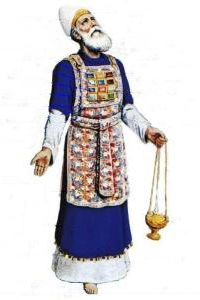
\includegraphics[width=50mm,scale=1.5]{Extras/Melchisedec.jpg}
\vspace{0.4in}  % Create a title for the document and write it in bold font
\LARGE{\textbf{\date}} % Again, do a line break
\linebreak 
% Create a subtitle \large{with Outlines, Statistics, Cross References, and Notes}
\vspace{0.5in}
\begin{flushleft}
\LARGE{Day \#50: Saturday, 19 February 2022 LITE  \\}\vspace{0.25in}
\LARGE{Numbers 28-30 Psalm 50 Proverb 19}
\end{flushleft}
\vspace{0.6in}
\bigskip

\normalsize{Xenia, Oh.\\}
\normalsize{created: \today}
\vspace{1.3in}

\end{flushright}
\end{titlepage}

\newpage 
\tableofcontents\hypertarget{TOC}{}
\listoffigures
\listoftables

\hyphenation{A-bim-e-lech bre-thren E-phra-im  Gib-e-o-nites Jer-u-sa-lem through-out Phil-i-stines The-o-phil-us Am-a-le-kites ven-geance Mesh-el-e-mi-ah onan-ism Phar-a-oh thoughts grev-ous-ness Hach-a-liah adul-ter-er Shad-rach}

%%%%%%%%%%%%%%%%% EXTRA COLORS
%%%%%%%%%%%%%%%%% EXTRA COLORS
%%%%%%%%%%%%%%%%% EXTRA COLORS
\definecolor{champagne}{rgb}{0.97,0.91,0.81}
\definecolor{bone}{rgb}{0.89,0.85,0.79}

\definecolor{ForestGreen}{rgb}{0.00,0.29,0.098}
\definecolor{GIVING}{cmyk}{1,0.0,0.72,.1}

\definecolor{MLPE}{cmyk}{1,1,0,.45}
\definecolor{SOCCER}{cmyk}{.77, 0, .42, .49}
\definecolor{PAYBILL}{cmyk}{0,0.83,0.76,0.07}
\definecolor{SERMON}{cmyk}{.14,.9,0,.30} % aka seance \href{http://www.flatuicolorpicker.com/purple-cmyk-color-model/}{seance}
\definecolor{BIBLE}{cmyk}{0,.17,.74,.17}
\definecolor{WORKBLUE}{cmyk}{1, .5, 0, .6}
\definecolor{myOrange}{cmyk}{0, .4, .98, .03}
\definecolor{myTan}{cmyk}{0.0,.07,.17,.10}
\definecolor{myRed}{cmyk}{0,1,1,0}
\definecolor{myWhite}{cmyk}{0,0,0,0}
\definecolor{BLUESoD}{cmyk}{.97,.84,0,.04}
\definecolor{WHITE}{cmyk}{0,0,0,0}
\definecolor{OLDGOLD}{cmyk}{0.05,0.3,1.00,0}
\definecolor{CASTLETON}{cmyk}{1,0,0.31,0.66}
\definecolor{cadmiumgreen}{rgb}{0.0, 0.42, 0.24}
\definecolor{jungle}{rgb}{0.203,0.4882,0.1718}
\definecolor{MYGOLD}{rgb}{1,.84,0}

\definecolor{MYLIGHTGRAY}{rgb}{.85,.85,.85}

\definecolor{codegreen}{rgb}{0,0.6,0}
\definecolor{codegray}{rgb}{0.5,0.5,0.5}
\definecolor{codepurple}{rgb}{0.58,0,0.82}
\definecolor{backcolour}{rgb}{0.95,0.95,0.92}


\mdfdefinestyle{MyFrame}{%
    linecolor=blue,
    outerlinewidth=2pt,
    roundcorner=5pt,
    innertopmargin=\baselineskip,
    innerbottommargin=\baselineskip,
    innerrightmargin=10pt,
    innerleftmargin=10pt,
    backgroundcolor=gray!25!white}


\mdfdefinestyle{MyFrame2}{%
    linecolor=black,
    outerlinewidth=2pt,
    roundcorner=5pt,
    innertopmargin=\baselineskip,
    innerbottommargin=\baselineskip,
    innerrightmargin=10pt,
    innerleftmargin=10pt,
    backgroundcolor=yellow!25!white}


%%%%%
%% for PFTTIS list
%%%%%

%%% And Joseph said unto
\index[PFTTIS]{And Joseph said unto!Genesis!Gen 40:008}
\index[PFTTIS]{And Joseph said unto!Genesis!Gen 40:012}
\index[PFTTIS]{And Joseph said unto!Genesis!Gen 41:025}
\index[PFTTIS]{And Joseph said unto!Genesis!Gen 42:014}
\index[PFTTIS]{And Joseph said unto!Genesis!Gen 42:018}
\index[PFTTIS]{And Joseph said unto!Genesis!Gen 44:015}
\index[PFTTIS]{And Joseph said unto!Genesis!Gen 45:003}
\index[PFTTIS]{And Joseph said unto!Genesis!Gen 45:004}
\index[PFTTIS]{And Joseph said unto!Genesis!Gen 46:031}
\index[PFTTIS]{And Joseph said unto!Genesis!Gen 48:009}
\index[PFTTIS]{And Joseph said unto!Genesis!Gen 48:018}
\index[PFTTIS]{And Joseph said unto!Genesis!Gen 50:019}
\index[PFTTIS]{And Joseph said unto!Genesis!Gen 50:024}


%%% a shadow
\index[PFTTIS]{a shadow!1Chronicles!1Chr 029:15}
\index[PFTTIS]{a shadow!Job!Job 008:09}
\index[PFTTIS]{a shadow!Job!Job 014:02}
\index[PFTTIS]{a shadow!Job!Job 017:07}
\index[PFTTIS]{a shadow!Psalm!Psa 102:011}
\index[PFTTIS]{a shadow!Psalm!Psa 144:004}
\index[PFTTIS]{a shadow!Ecclesiastes!Eccl 006:012}
\index[PFTTIS]{a shadow!Ecclesiastes!Eccl 008:013}
\index[PFTTIS]{a shadow!Isaiah!Isa 04:006}
\index[PFTTIS]{a shadow!Isaiah!Isa 25:004}
\index[PFTTIS]{a shadow!Jonah!Jnh 04:06}
\index[PFTTIS]{a shadow!Colossians!Col 02:017}
\index[PFTTIS]{a shadow!Hebews!Heb 10:001}

%%% blessed is the man
\index[PFTTIS]{blessed is the man!Psalm!Psa 001:001}
\index[PFTTIS]{blessed is the man!Psalm!Psa 032:002}
\index[PFTTIS]{blessed is the man!Psalm!Psa 034:008}
\index[PFTTIS]{blessed is the man!Psalm!Psa 065:004}
\index[PFTTIS]{blessed is the man!Psalm!Psa 084:005}
\index[PFTTIS]{blessed is the man!Psalm!Psa 084:012}
\index[PFTTIS]{blessed is the man!Psalm!Psa 094:012}
\index[PFTTIS]{blessed is the man!Psalm!Psa 112:001}
\index[PFTTIS]{blessed is the man!Proverbs!Pro 008:034}
\index[PFTTIS]{blessed is the man!Isaiah!Isa 056:002}
\index[PFTTIS]{blessed is the man!Jeremiah!Jer 017:007}
\index[PFTTIS]{blessed is the man!Romans!Rom 004:008}
\index[PFTTIS]{blessed is the man!James!Jam 001:012}


%%% carry them
\index[PFTTIS]{carry them!Leviticus!Lev 14:045}
\index[PFTTIS]{carry them!Numbers!Num 11:012}
\index[PFTTIS]{carry them!Joshua!Jsh 04:003}
\index[PFTTIS]{carry them!1Samuel!1Sam 20:040}
\index[PFTTIS]{carry them!1Kings!1Kng 08:046}
\index[PFTTIS]{carry them!2Chronicles!2Chr 06:036}
\index[PFTTIS]{carry them!Ezra!Ezra 05:015}
\index[PFTTIS]{carry them!Isaiah!Isa 40:011}
\index[PFTTIS]{carry them!Isaiah!Isa 41:016}
\index[PFTTIS]{carry them!Isaiah!Isa 57:013}
\index[PFTTIS]{carry them!Jeremiah!Jer 20:004}
\index[PFTTIS]{carry them!Jeremiah!Jer 20:005}
\index[PFTTIS]{carry them!Jeremiah!Jer 43:012}


\index[PFTTIS]{good tidings!2Samuel!2Sam 18:027}
\index[PFTTIS]{good tidings!1Kings!1Ki 01:042}
\index[PFTTIS]{good tidings!2Kings!2Ki 07:009 (2x)}
\index[PFTTIS]{good tidings!Isaiah!Isa 40:009 (2x)}
\index[PFTTIS]{good tidings!Isaiah!Isa 41:007}
\index[PFTTIS]{good tidings!Isaiah!Isa 52:007}
\index[PFTTIS]{good tidings!Isaiah!Isa 61:001}
\index[PFTTIS]{good tidings!Nahum!Nah 01:005}
\index[PFTTIS]{good tidings!Luke!Lk 02:010}
\index[PFTTIS]{good tidings!1Thessalonians!1Thess 03:006}


%%% dead body
\index[PFTTIS]{dead body!Leviticus!Lev 21:011}
\index[PFTTIS]{dead body!Numbers!Num 06:006}
\index[PFTTIS]{dead body!Numbers!Num 09:006}
\index[PFTTIS]{dead body!Numbers!Num 09:007}
\index[PFTTIS]{dead body!Numbers!Num 09:010}
\index[PFTTIS]{dead body!Numbers!Num 09:011}
\index[PFTTIS]{dead body!Numbers!Num 09:013}
\index[PFTTIS]{dead body!Numbers!Num 09:016}
\index[PFTTIS]{dead body!2Kings!2Ki 08:005}
\index[PFTTIS]{dead body!Isaiah!Isa 26:019}
\index[PFTTIS]{dead body!Jeremiah!Jer 26:023}
\index[PFTTIS]{dead body!Jeremiah!Jer 36:030}
\index[PFTTIS]{dead body!Haggai!Hag 02:013}

%%% great sea
\index[PFTTIS]{great sea!Numbers!Num 34:006}
\index[PFTTIS]{great sea!Numbers!Num 34:007}
\index[PFTTIS]{great sea!Joshua!Jos 01:004}
\index[PFTTIS]{great sea!Joshua!Jos 09:001}
\index[PFTTIS]{great sea!Joshua!Jos 15:012}
\index[PFTTIS]{great sea!Joshua!Jos 15:047}
\index[PFTTIS]{great sea!Joshua!Jos 23:004}
\index[PFTTIS]{great sea!Ezekiel!Eze 47:010}
\index[PFTTIS]{great sea!Ezekiel!Eze 47:015}
\index[PFTTIS]{great sea!Ezekiel!Eze 47:019}
\index[PFTTIS]{great sea!Ezekiel!Eze 47:020}
\index[PFTTIS]{great sea!Ezekiel!Eze 48:028}
\index[PFTTIS]{great sea!Daniel!Dan 07:002}


%%% have forsaken me
\index[PFTTIS]{have forsaken me!Judges!Jdg 10:013}
\index[PFTTIS]{have forsaken me!1Samuel!1Sam 08:008}
\index[PFTTIS]{have forsaken me!1Kings!1Ki 11:033}
\index[PFTTIS]{have forsaken me!2Kings!2Ki 22:017}
\index[PFTTIS]{have forsaken me!2Chronicles!2Chr 12:005}
\index[PFTTIS]{have forsaken me!2Chronicles!2Chr 34:025}
\index[PFTTIS]{have forsaken me!Jeremiah!Jer 01:016}
\index[PFTTIS]{have forsaken me!Jeremiah!Jer 02:013}
\index[PFTTIS]{have forsaken me!Jeremiah!Jer 05:007}
\index[PFTTIS]{have forsaken me!Jeremiah!Jer 05:019}
\index[PFTTIS]{have forsaken me!Jeremiah!Jer 16:011 (2x)}
\index[PFTTIS]{have forsaken me!Jeremiah!Jer 19:004}

%%% no king
\index[PFTTIS]{no king!Judges!Jdg 17:06}
\index[PFTTIS]{no king!Judges!Jdg 18:01}
\index[PFTTIS]{no king!Judges!Jdg 19:01}
\index[PFTTIS]{no king!Judges!Jdg 21:25}
\index[PFTTIS]{no king!1Kings!1Ki 22:47}
\index[PFTTIS]{no king!2Kings!2Ki 23:25}
\index[PFTTIS]{no king!Nehemiah!Neh 13:26}
\index[PFTTIS]{no king!Psalms!Psa 033:016}
\index[PFTTIS]{no king!Proverbs!Pro 30:27}
\index[PFTTIS]{no king!Daniel!Dan 02:10}
\index[PFTTIS]{no king!Hosea!Hos 10:03}
\index[PFTTIS]{no king!Micah!Mic 04:09}
\index[PFTTIS]{no king!John!Jhn 19:15}


%%% rebellious house
\index[PFTTIS]{rebellious house!Exodus!Exo 02:005}
\index[PFTTIS]{rebellious house!Exodus!Exo 02:006}
\index[PFTTIS]{rebellious house!Exodus!Exo 02:008}
\index[PFTTIS]{rebellious house!Exodus!Exo 03:009}
\index[PFTTIS]{rebellious house!Exodus!Exo 03:026}
\index[PFTTIS]{rebellious house!Exodus!Exo 03:027}
\index[PFTTIS]{rebellious house!Exodus!Exo 12:002 (2x)}
\index[PFTTIS]{rebellious house!Exodus!Exo 12:003}
\index[PFTTIS]{rebellious house!Exodus!Exo 12:009}
\index[PFTTIS]{rebellious house!Exodus!Exo 12:025}
\index[PFTTIS]{rebellious house!Exodus!Exo 17:012}
\index[PFTTIS]{rebellious house!Exodus!Exo 24:003}

%%% seek him
\index[PFTTIS]{seek him!Deuteronomy!Deu 04:029}\index[PFTTIS]{seek him!1Samuel!1Sam 23:025}
\index[PFTTIS]{seek him!1Chronicles!1Chr 28:009}
\index[PFTTIS]{seek him!2Chronicles!1Chr 15:002}
\index[PFTTIS]{seek him!Ezra!Ezr 08:022}
\index[PFTTIS]{seek him!Psalms!Psa 022:026}
\index[PFTTIS]{seek him!Psalms!Psa 024:006}
\index[PFTTIS]{seek him!Psalms!Psa 119:002}
\index[PFTTIS]{seek him!SoS!SoS 03:002}
\index[PFTTIS]{seek him!SoS!SoS 06:001}
\index[PFTTIS]{seek him!Hosea!Hos 07:010}
\index[PFTTIS]{seek him!Amos!Amo 05:008}
\index[PFTTIS]{seek him!Hebrews!Heb 11:0063}


%%% seek ye
\index[PFTTIS]{seek ye!Isaiah!Isa 34:016}
\index[PFTTIS]{seek ye!Isaiah!Isa 45:019}
\index[PFTTIS]{seek ye!Isaiah!Isa 55:006}
\index[PFTTIS]{seek ye!Amos!Amos 5:004}
\index[PFTTIS]{seek ye!John!John 1:38}
\index[PFTTIS]{seek ye!John!John 18:4}
\index[PFTTIS]{seek ye!John!John 18:7}
\index[PFTTIS]{seek ye!Matthew!Matt 6:33}
\index[PFTTIS]{seek ye!Numbers!Num 16:10}
\index[PFTTIS]{seek ye!Luke!Luke 12:31}
\index[PFTTIS]{seek ye!Luke!Luke 24:5}
\index[PFTTIS]{seek ye!Psalm!Psa 27:8}
\index[PFTTIS]{seek ye!Zephaniah!Zeph 2:3}

%%% the uncircumcised
\index[PFTTIS]{the uncircumcised!Genesis!Gen 17:014}
\index[PFTTIS]{the uncircumcised!Judges!Jdg 14:003}
\index[PFTTIS]{the uncircumcised!Judges!Jdg 15:018}
\index[PFTTIS]{the uncircumcised!2Samuel!2Sam 01:020}
\index[PFTTIS]{the uncircumcised!Isaiah!Isa 02:001}
\index[PFTTIS]{the uncircumcised!Jeremiah!Jer 09:025}
\index[PFTTIS]{the uncircumcised!Ezekiel!Eze 28:010}
\index[PFTTIS]{the uncircumcised!Ezekiel!Eze 31:018}
\index[PFTTIS]{the uncircumcised!Ezekiel!Eze 32:019}
\index[PFTTIS]{the uncircumcised!Ezekiel!Eze 32:027}
\index[PFTTIS]{the uncircumcised!Ezekiel!Eze 32:028}
\index[PFTTIS]{the uncircumcised!Ezekiel!Eze 32:029}
\index[PFTTIS]{the uncircumcised!Ezekiel!Eze 32:032}

%%% worship him
\index[PFTTIS]{worship him!Psalms!Psa 97:007}
\index[PFTTIS]{worship him!Zephaniah!Zeph 02:011}
\index[PFTTIS]{worship him!Matthew!Matt 02:002}
\index[PFTTIS]{worship him!Matthew!Matt 02:008}
\index[PFTTIS]{worship him!John!John 04:023}
\index[PFTTIS]{worship him!John!John 04:024 (2x)} 
\index[PFTTIS]{worship him!Acts!Acts 17:023}
\index[PFTTIS]{worship him!Hebrews!Heb 01:006}
\index[PFTTIS]{worship him!Revelation!Rev 04:010}
\index[PFTTIS]{worship him!Revelation!Rev 13:008}
\index[PFTTIS]{worship him!Revelation!Rev 14:007}
\index[PFTTIS]{worship him!Revelation!Rev 19:010}


%%%%%
%% for PFTTIS list
%%%%%

%%% afflictions
\index[WFTTIS]{afflictions!Psalms!Psa 34:019}
\index[WFTTIS]{afflictions!Psalms!Psa 132:001}
\index[WFTTIS]{afflictions!Acts!Acts 07:010}
\index[WFTTIS]{afflictions!Acts!Acts 20:023}
\index[WFTTIS]{afflictions!2Corinthians!2Cor 06:004}
\index[WFTTIS]{afflictions!Colossians!Col 01:024}
\index[WFTTIS]{afflictions!1Thessalonians!1Thess 03:003}
\index[WFTTIS]{afflictions!2Timothy!2Tim 01:008}
\index[WFTTIS]{afflictions!2Timothy!2Tim 03:011}
\index[WFTTIS]{afflictions!2Timothy!2Tim 04:005}
\index[WFTTIS]{afflictions!Hebrews!Heb 10:032}
\index[WFTTIS]{afflictions!Hebrews!Heb 10:033}
\index[WFTTIS]{afflictions!1Peter!1Pet 05:009}

%%% acsend
\index[WFTTIS]{acsend!Joshua!Jos 06:05}
\index[WFTTIS]{acsend!Psalm!Psa 024:003}
\index[WFTTIS]{acsend!Psalm!Psa 135:007}
\index[WFTTIS]{acsend!Psalm!Psa 139:008}
\index[WFTTIS]{acsend!Isaiah!Isa 14:013}
\index[WFTTIS]{acsend!Isaiah!Isa 14:014}
\index[WFTTIS]{acsend!Jeremiah!Jer 10:013}
\index[WFTTIS]{acsend!Jeremiah!Jer 51:016}
\index[WFTTIS]{acsend!Ezekiel!Eze 38:009}
\index[WFTTIS]{acsend!John!John 06:062}
\index[WFTTIS]{acsend!John!John 20:017}
\index[WFTTIS]{acsend!Romans!Rom 10:006}
\index[WFTTIS]{acsend!Revelation!Rev 17:008}

%%% Assyrian
\index[WFTTIS]{Assyrian!Isaiah!Isa 10:005}
\index[WFTTIS]{Assyrian!Isaiah!Isa 10:024}
\index[WFTTIS]{Assyrian!Isaiah!Isa 14:025}
\index[WFTTIS]{Assyrian!Isaiah!Isa 19:023}
\index[WFTTIS]{Assyrian!Isaiah!Isa 23:013}
\index[WFTTIS]{Assyrian!Isaiah!Isa 30:031}
\index[WFTTIS]{Assyrian!Isaiah!Isa 31:008}
\index[WFTTIS]{Assyrian!Isaiah!Isa 52:004}
\index[WFTTIS]{Assyrian!Ezekiel!Eze 31:003}
\index[WFTTIS]{Assyrian!Hosea!Hos 05:013}
\index[WFTTIS]{Assyrian!Hosea!Hos 11:005}
\index[WFTTIS]{Assyrian!Micah!Hos 05:005}
\index[WFTTIS]{Assyrian!Micah!Hos 05:006}

%%% blot
\index[WFTTIS]{blot!Exodus!Exo 32:032}
\index[WFTTIS]{blot!Exodus!Exo 32:033}
\index[WFTTIS]{blot!Numbers!Num 05:026}
\index[WFTTIS]{blot!Deuteronomy!Deut 09:014}
\index[WFTTIS]{blot!Deuteronomy!Deut 25:019}
\index[WFTTIS]{blot!Deuteronomy!Deut 29:020}
\index[WFTTIS]{blot!2Kings!2Ki 14:027}
\index[WFTTIS]{blot!Job!Job 31:007}
\index[WFTTIS]{blot!Psalms!Psa 51:001}
\index[WFTTIS]{blot!Psalms!Psa 51:009}
\index[WFTTIS]{blot!Proverbs!Pro 09:007}
\index[WFTTIS]{blot!Jeremiah!Jer 18:023}
\index[WFTTIS]{blot!Revelation!Rev 03:005}


%%% chain
\index[WFTTIS]{chain!Genesis!Gen 41:042}
\index[WFTTIS]{chain!1Kings!1Ki 07:017}
\index[WFTTIS]{chain!Psalms!Psa 73:006}
\index[WFTTIS]{chain!SoS!Sos 04:009}
\index[WFTTIS]{chain!Lamentations!Lam 03:007}
\index[WFTTIS]{chain!Ezekiel!Eze 07:023}
\index[WFTTIS]{chain!Ezekiel!Eze 16:011}
\index[WFTTIS]{chain!Daniel!Dan 05:007}
\index[WFTTIS]{chain!Daniel!Dan 05:016}
\index[WFTTIS]{chain!Daniel!Dan 05:029}
\index[WFTTIS]{chain!Acts!Acts 28:020}
\index[WFTTIS]{chain!2Timothy!2Tim 01:016}
\index[WFTTIS]{chain!Revelation!Rev 20:001}


%%% controversy
\index[WFTTIS]{controversy!Deuteronomy!Deu 17:008}
\index[WFTTIS]{controversy!Deuteronomy!Deu 19:017}
\index[WFTTIS]{controversy!Deuteronomy!Deu 21:005}
\index[WFTTIS]{controversy!Deuteronomy!Deu 25:001}
\index[WFTTIS]{controversy!2Samuel!2Sam 15:002}
\index[WFTTIS]{controversy!Isaiah!Isa 34:008}
\index[WFTTIS]{controversy!Jeremiah!Jer 25:031}
\index[WFTTIS]{controversy!Ezekiel!Eze 44:024}
\index[WFTTIS]{controversy!Hosea!Hos 04:001}
\index[WFTTIS]{controversy!Hosea!Hos 12:002}
\index[WFTTIS]{controversy!Micah!Mic 06:002 (2x)}
\index[WFTTIS]{controversy!1Timothy!1Tim 03:016}


%%% Dagon/Dagon's
\index[WFTTIS]{Dagon!Judges!Jdg 16:023}
\index[WFTTIS]{Dagon!1Samuel!1Sam 05:002 (2x)}
\index[WFTTIS]{Dagon!1Samuel!1Sam 05:003 (2x)}
\index[WFTTIS]{Dagon!1Samuel!1Sam 05:004 (3x)}
\index[WFTTIS]{Dagon!1Samuel!1Sam 05:005 (3x)}
\index[WFTTIS]{Dagon!1Samuel!1Sam 05:007}
\index[WFTTIS]{Dagon!1Chronicles!1Chr 10:010}

%%% disobedient
\index[WFTTIS]{disobedient!1Kings!1Ki 13:026}
\index[WFTTIS]{disobedient!Nehemiah!Neh 09:026}
\index[WFTTIS]{disobedient!Luke!Luke 01:017}
\index[WFTTIS]{disobedient!Acts!Acts 26:019}
\index[WFTTIS]{disobedient!Romans!Rom 01:030}
\index[WFTTIS]{disobedient!Romans!Rom 10:021}
\index[WFTTIS]{disobedient!1Timothy!1Tim 01:009}
\index[WFTTIS]{disobedient!2Timothy!2Tim 03:002}
\index[WFTTIS]{disobedient!Titus!Titus 01:016}
\index[WFTTIS]{disobedient!Titus!Titus 03:003}
\index[WFTTIS]{disobedient!1Peter!1Pet 02:007}
\index[WFTTIS]{disobedient!1Peter!1Pet 02:008}
\index[WFTTIS]{disobedient!1Peter!1Pet 03:020}


%%% doubt
\index[WFTTIS]{doubt!Genesis!Gen 37:033}
\index[WFTTIS]{doubt!Deuteronomy!Deu 28:066}
\index[WFTTIS]{doubt!Job!Job 12:002}
\index[WFTTIS]{doubt!Matthew!Matt 14:031}
\index[WFTTIS]{doubt!Matthew!Matt 21:021}
\index[WFTTIS]{doubt!Mark!Mk 11:023}
\index[WFTTIS]{doubt!Luke!Lk 11:020}
\index[WFTTIS]{doubt!John!Jhn 10:024}
\index[WFTTIS]{doubt!Acts!Acts 02:012}
\index[WFTTIS]{doubt!Acts!Acts 28:004}
\index[WFTTIS]{doubt!1Corinthians!1Cor 09:010}
\index[WFTTIS]{doubt!Galatians!Gal 04:020}
\index[WFTTIS]{doubt!1John!1Jhn 02:019}


%%% dungeon
\index[WFTTIS]{dungeon!Genesis!Gen 40:015}
\index[WFTTIS]{dungeon!Genesis!Gen 41:014}
\index[WFTTIS]{dungeon!Exodus!Exo 12:029}
\index[WFTTIS]{dungeon!Jeremiah!Jer 37:016}
\index[WFTTIS]{dungeon!Jeremiah!Jer 38:006 (2x)}
\index[WFTTIS]{dungeon!Jeremiah!Jer 38:007}
\index[WFTTIS]{dungeon!Jeremiah!Jer 38:009}
\index[WFTTIS]{dungeon!Jeremiah!Jer 38:010}
\index[WFTTIS]{dungeon!Jeremiah!Jer 38:011}
\index[WFTTIS]{dungeon!Jeremiah!Jer 38:013}
\index[WFTTIS]{dungeon!Lamentations!Lam 03:053}
\index[WFTTIS]{dungeon!Lamentations!Lam 03:055}


%%% error
\index[WFTTIS]{error!2Samuel!2Sam 06:007}
\index[WFTTIS]{error!Job!Job 19:004}
\index[WFTTIS]{error!Ecclesiastes!Ecc 05:006}
\index[WFTTIS]{error!Ecclesiastes!Ecc 10:005}
\index[WFTTIS]{error!Isaiah!Isa 32:006}
\index[WFTTIS]{error!Daniel!Dan 06:004}
\index[WFTTIS]{error!Matthew!Matt 27:064}
\index[WFTTIS]{error!Romans!Rom 01:027}
\index[WFTTIS]{error!James!Jam 05:020}
\index[WFTTIS]{error!2Peter!2Pet 02:018}
\index[WFTTIS]{error!2Peter!2Pet 03:017}
\index[WFTTIS]{error!1John!1Jn 04:006}
\index[WFTTIS]{error!Jude!Jude 01:011}

%%% fourish
\index[WFTTIS]{fourish!Psalms!Psa 072:007}
\index[WFTTIS]{fourish!Psalms!Psa 072:016}
\index[WFTTIS]{fourish!Psalms!Psa 092:007}
\index[WFTTIS]{fourish!Psalms!Psa 092:012}
\index[WFTTIS]{fourish!Psalms!Psa 092:013}
\index[WFTTIS]{fourish!Psalms!Psa 132:018}
\index[WFTTIS]{fourish!Proverbs!Pro 11:28}
\index[WFTTIS]{fourish!Proverbs!Pro 14:11}
\index[WFTTIS]{fourish!Ecclesiastes!Ecc 12:05}
\index[WFTTIS]{fourish!SongOfSolomon!SOS 07:12}
\index[WFTTIS]{fourish!Isaiah!Isa 17:11}
\index[WFTTIS]{fourish!Isaiah!Isa 66:14}
\index[WFTTIS]{fourish!Ezekiel!Eze 17:24}




%%% giants
\index[WFTTIS]{giants!Genesis!Gen 06:004}
\index[WFTTIS]{giants!Numbers!Num 13:033}
\index[WFTTIS]{giants!Deuteronomy!Deut 02:011}
\index[WFTTIS]{giants!Deuteronomy!Deut 02:021}
\index[WFTTIS]{giants!Deuteronomy!Deut 03:011}
\index[WFTTIS]{giants!Deuteronomy!Deut 03:013}
\index[WFTTIS]{giants!Joshua!Josh 12:004}
\index[WFTTIS]{giants!Joshua!Josh 13:012}
\index[WFTTIS]{giants!Joshua!Josh 15:008}
\index[WFTTIS]{giants!Joshua!Josh 17:015}
\index[WFTTIS]{giants!Joshua!Josh 16:016}

%%% good man
\index[WFTTIS]{good man!2 Samuel!2Sa 18:27}
%(1) Psalms 37:23 [5]
%(1) Psalms 112:5 [2]
%(1) Proverbs 12:2 [2]
%(1) Proverbs 13:22 [2]
%(1) Proverbs 14:14 [14]
%(1) Micah 7:2 [2]
%(1) Matthew 12:35 [2]
%(1) Luke 6:45 [2]
%(1) Luke 23:50 [15]
%(1) John 7:12 [17]
%(1) Acts 11:24 [5]
%(1) Romans 5:7 [14]

%%% Hinnom
\index[WFTTIS]{Hinnom!Joshua!Jsh 15:008}
\index[WFTTIS]{Hinnom!Joshua!Jsh 18:016}
\index[WFTTIS]{Hinnom!2Kings!2Ki 23:010}
\index[WFTTIS]{Hinnom!2Chronicles!2Chr 28:003}
\index[WFTTIS]{Hinnom!2Chronicles!2Chr 33:006}
\index[WFTTIS]{Hinnom!Nehemiah!Neh 11:030}
\index[WFTTIS]{Hinnom!Jeremiah!Jer 07:031}
\index[WFTTIS]{Hinnom!Jeremiah!Jer 07:032}
\index[WFTTIS]{Hinnom!Jeremiah!Jer 19:002}
\index[WFTTIS]{Hinnom!Jeremiah!Jer 19:006}
\index[WFTTIS]{Hinnom!Jeremiah!Jer 32:035}

%%% inclined
\index[WFTTIS]{inclined!Judges!Jdg 09:003}
\index[WFTTIS]{inclined!Psalms!Psa 040:001}
\index[WFTTIS]{inclined!Psalms!Psa 116:002}
\index[WFTTIS]{inclined!Psalms!Psa 119:112}
\index[WFTTIS]{inclined!Proverbs!Pro 05:13}
\index[WFTTIS]{inclined!Jeremiah!Jer 07:24}
\index[WFTTIS]{inclined!Jeremiah!Jer 07:26}
\index[WFTTIS]{inclined!Jeremiah!Jer 11:08}
\index[WFTTIS]{inclined!Jeremiah!Jer 17:23}
\index[WFTTIS]{inclined!Jeremiah!Jer 25:04}
\index[WFTTIS]{inclined!Jeremiah!Jer 34:14}
\index[WFTTIS]{inclined!Jeremiah!Jer 35:15}
\index[WFTTIS]{inclined!Jeremiah!Jer 44:05}


%%% laughed
\index[WFTTIS]{laughed!Genesis!Gen 17:017}
\index[WFTTIS]{laughed!Genesis!Gen 18:012}
\index[WFTTIS]{laughed!Genesis!Gen 18:015}
\index[WFTTIS]{laughed!2Kings!2Ki 19:021}
\index[WFTTIS]{laughed!2Chronicles!2Chr 30:010}
\index[WFTTIS]{laughed!Nehemiah!Neh 02:019}
\index[WFTTIS]{laughed!Job!Job 12:004}
\index[WFTTIS]{laughed!Job!Job 29:024}
\index[WFTTIS]{laughed!Isaiah!Isa 37:022}
\index[WFTTIS]{laughed!Ezekiel!Ezek 23:032}
\index[WFTTIS]{laughed!Matthew!Matt 09:024}
\index[WFTTIS]{laughed!Mark!Mk 05:040}
\index[WFTTIS]{laughed!Luke!Lk 08:053}

%%% liar
\index[WFTTIS]{liar!Job!Job 24:025}
\index[WFTTIS]{liar!Proverbs!Pro 17:004}
\index[WFTTIS]{liar!Proverbs!Pro 19:022}
\index[WFTTIS]{liar!Proverbs!Pro 30:006}
\index[WFTTIS]{liar!Jeremiah!Jer 15:018}
\index[WFTTIS]{liar!John!Jhn 08:044}
\index[WFTTIS]{liar!John!Jhn 08:055}
\index[WFTTIS]{liar!Romans!Rom 03:004}
\index[WFTTIS]{liar!1John!1Jhn 01:010}
\index[WFTTIS]{liar!1John!1Jhn 02:004}
\index[WFTTIS]{liar!1John!1Jhn 02:022}
\index[WFTTIS]{liar!1John!1Jhn 04:020}
\index[WFTTIS]{liar!1John!1Jhn 05:010}

%%% palsy
\index[WFTTIS]{palsy!Matthew!Matt 04:024}
\index[WFTTIS]{palsy!Matthew!Matt 08:006}
\index[WFTTIS]{palsy!Matthew!Matt 09:002}
\index[WFTTIS]{palsy!Matthew!Matt 09:006}
\index[WFTTIS]{palsy!Mark!Mk 02:003}
\index[WFTTIS]{palsy!Mark!Mk 02:004}
\index[WFTTIS]{palsy!Mark!Mk 02:005}
\index[WFTTIS]{palsy!Mark!Mk 02:009}
\index[WFTTIS]{palsy!Mark!Mk 02:010}
\index[WFTTIS]{palsy!Luke!Lk 05:018}
\index[WFTTIS]{palsy!Luke!Lk 05:024}
\index[WFTTIS]{palsy!Acts!Acts 09:033}

%%% Profitable
\index[WFTTIS]{profitable!Job!Job 22:002 (2x)}
\index[WFTTIS]{profitable!Ecclesiastes!Ecc 10:010}
\index[WFTTIS]{profitable!Isaiah!Isa 44:010}
\index[WFTTIS]{profitable!Jeremiah!Jer 13:007}
\index[WFTTIS]{profitable!Matthew!Matt 05:029}
\index[WFTTIS]{profitable!Matthew!Matt 05:030}
\index[WFTTIS]{profitable!Acts!Acts 20:020}
\index[WFTTIS]{profitable!1Timothy!1Tim 04:008}
\index[WFTTIS]{profitable!2Timothy!2Tim 03:016}
\index[WFTTIS]{profitable!2Timothy!2Tim 04:011}
\index[WFTTIS]{profitable!Titus!Titus 03:008}
\index[WFTTIS]{profitable!Philemon!Phlm 01:011}

%%% Rechab
\index[WFTTIS]{Rechab!2Samuel!2Sam 04:002}
\index[WFTTIS]{Rechab!2Samuel!2Sam 04:005}
\index[WFTTIS]{Rechab!2Samuel!2Sam 04:006}
\index[WFTTIS]{Rechab!2Samuel!2Sam 04:009}
\index[WFTTIS]{Rechab!2KIngs!2Ki 10:015}
\index[WFTTIS]{Rechab!2KIngs!2Ki 10:023}
\index[WFTTIS]{Rechab!1Chronicles!1Chr 02:055}
\index[WFTTIS]{Rechab!Nehemiah!Neh 03:014}
\index[WFTTIS]{Rechab!Jeremiah!Jer 35:006}
\index[WFTTIS]{Rechab!Jeremiah!Jer 35:008}
\index[WFTTIS]{Rechab!Jeremiah!Jer 35:014}
\index[WFTTIS]{Rechab!Jeremiah!Jer 35:016}
\index[WFTTIS]{Rechab!Jeremiah!Jer 35:019}

%%% serpents
\index[WFTTIS]{serpents!Exodus!Exo 07:012}
\index[WFTTIS]{serpents!Numbers!Num 21:006}
\index[WFTTIS]{serpents!Numbers!Num 21:007}
\index[WFTTIS]{serpents!Deuteronomy!Deu 08:015}
\index[WFTTIS]{serpents!Deuteronomy!Deu 32:024}
\index[WFTTIS]{serpents!Jeremiah!Jer 08:017}
\index[WFTTIS]{serpents!Matthew!Matt 10:016}
\index[WFTTIS]{serpents!Matthew!Matt 23:033}
\index[WFTTIS]{serpents!Mark!Mk 16:018}
\index[WFTTIS]{serpents!Luke!Lk 10:019}
\index[WFTTIS]{serpents!1Corinthians!1Cor 10:009}
\index[WFTTIS]{serpents!James!Jas 03:007}
\index[WFTTIS]{serpents!Revelation!Rev 09:019}

%%% short
\index[WFTTIS]{short!Numbers!Num 11:023}
\index[WFTTIS]{short!2Kings!2Ki 10:032}
\index[WFTTIS]{short!Job!Job 17:012}
\index[WFTTIS]{short!Job!Job 20:005}
\index[WFTTIS]{short!Psalms!Psa 89:047}
\index[WFTTIS]{short!Romans!Rom 03:023}
\index[WFTTIS]{short!Romans!Rom 09:028  (2x)}
\index[WFTTIS]{short!1Corinthians!1Cor 07:029}
\index[WFTTIS]{short!1Thessalonians!1Thess 02:017}
\index[WFTTIS]{short!Hebrews!Heb 04:001}
\index[WFTTIS]{short!Revelation!Rev 12:012}
\index[WFTTIS]{short!Revelation!Rev 17:010}

%%% smiteth
\index[WFTTIS]{smiteth!Exodus!Exo 21:012}
\index[WFTTIS]{smiteth!Exodus!Exo 21:15}
\index[WFTTIS]{smiteth!Deuteronomy!Dt 25:11}
\index[WFTTIS]{smiteth!Deuteronomy!Dt 27:24}
\index[WFTTIS]{smiteth!Joshua!Jsh 15:16}
\index[WFTTIS]{smiteth!Judges!Jdg 15:16}
\index[WFTTIS]{smiteth!2 Samuel!2Sa 05:08}
\index[WFTTIS]{smiteth!1Chronicles!1Chr 11:06}
\index[WFTTIS]{smiteth!Job!1Chr 26:12}
\index[WFTTIS]{smiteth!Isaiah!Isa 09:13}
\index[WFTTIS]{smiteth!Lamentations!Lam 03:30}
\index[WFTTIS]{smiteth!Ezekiel!Eze 07:09}
\index[WFTTIS]{smiteth!Luke!Lk 06:29}



%%% vanities
\index[WFTTIS]{vanities!Deuteronomy!Deut 21:021}
\index[WFTTIS]{vanities!1Kings!1Ki 16:013}
\index[WFTTIS]{vanities!1Kings!1Ki 16:026}
\index[WFTTIS]{vanities!Psalms!Psa 031:006}
\index[WFTTIS]{vanities!Ecclesiastes!Ecc 01:002 (2x)}
\index[WFTTIS]{vanities!Ecclesiastes!Ecc 05:007}
\index[WFTTIS]{vanities!Ecclesiastes!Ecc 12:008}
\index[WFTTIS]{vanities!Jeremiah!Jer 08:019}
\index[WFTTIS]{vanities!Jeremiah!Jer 10:008}
\index[WFTTIS]{vanities!Jeremiah!Jer 14:022}
\index[WFTTIS]{vanities!Jonah!Jnh 02:008}
\index[WFTTIS]{vanities!Acts!Acts 14:015}



%%%%%
%% for PFTTIS list
%%%%%

%%% worm
\index[WFITV]{worm!Exodus!Exo 16:024}
\index[WFITV]{worm!Job!Job 17:014}
\index[WFITV]{worm!Job!Job 24:029}
\index[WFITV]{worm!Job!Job 25:005 (2x)}
\index[WFITV]{worm!Psalms!Psa 022:006}
\index[WFITV]{worm!Isaiah!Isa 14:011}
\index[WFITV]{worm!Isaiah!Isa 41:014}
\index[WFITV]{worm!Isaiah!Isa 51:008}
\index[WFITV]{worm!Isaiah!Isa 66:024}
\index[WFITV]{worm!Jonah!Jnh 04:007}
\index[WFITV]{worm!Mark!Mk 09:044}
\index[WFITV]{worm!Mark!Mk 09:046}
\index[WFITV]{worm!Mark!Mk 09:048}


%\subsubsection{Title}
%\textbf{Introduction:} Isaiah 46 
%\index[speaker]{Speaker!Isaiah 49 (Title}
%\index[series]{Book (Speaker)!IPassage (Title)}
%\index[date]{2017/07/09!Isaiah 49 (Title)}
%\begin{compactenum}[I.]
%    \item  \textbf{Point} \index[scripture]{Isaiah!IPassage} (IPassage)
%\end{compactenum}




  



\chapter{Numbers 28}
%[cmyk]{0.99998,1,0,0}{


\marginpar{\scriptsize \centering \fcolorbox{bone}{lime}{\textbf{OFFERINGS \& MORE OF THEM}}\\ (Numbers 28)
\begin{compactenum}[I.][8]
    \item \textbf{Aroma} \index[scripture]{Numbers!Num 28:02}\index[scripture]{Numbers!Num 28:06} \index[scripture]{Numbers!Num 28:08}\index[scripture]{Numbers!Num 28:13}\index[scripture]{Numbers!Num 28:24}\index[scripture]{Numbers!Num 28:27}(Numbers 28:2, 6, 8, 13, 24, 27) -- sweet savour
    \item \textbf{Rituals} 
    \item \textbf{Rams} \index[scripture]{Numbers!Num 28:11}\index[scripture]{Numbers!Num 28:12} \index[scripture]{Numbers!Num 28:14}\index[scripture]{Numbers!Num 28:19}\index[scripture]{Numbers!Num 28:20}\index[scripture]{Numbers!Num 28:27}\index[scripture]{Numbers!Num 28:28}(Numbers 28:11, 12, 14, 19, 20, 27, 28) -
    \item \textbf{Repetition} -- \index[scripture]{Numbers!Num 28:31}(Numbers 28:31)
    \item \textbf{Remembrance} 
    \item \textbf{Reiteration} 
    \item \textbf{Requirement} 
    \item \textbf{Rest} \index[scripture]{Numbers!Num 28:26}(Numbers 28:26)
\end{compactenum}}

%%%%%%%%%%%%%%%%%%%%%%%%%%%%%%%%%%%%%%%%%
%%%%%%%%%%%%%%%%%%%%%%%%%%%%%%%%%%%%%%%%%
\footnote{\textcolor[rgb]{0.00,0.25,0.00}{\hyperlink{NumbersTOC}{Return to end of Table of Contents.}}}\footnote{\href{https://audiobible.com/bible/numbers_28.html}{\textcolor[cmyk]{0.99998,1,0,0}{Numbers 28 Audio}}}\textcolor[cmyk]{0.99998,1,0,0}{And \fcolorbox{bone}{bone}{the LORD} spake unto Moses, saying,}
[2] \textcolor[cmyk]{0.99998,1,0,0}{Command the children of Israel, and say unto them, My offering, \emph{and} my bread for my sacrifices made by fire, \emph{for} a sweet savour unto me, shall \fcolorbox{bone}{bone}{ye} observe to offer unto me in their due season.}
[3] \textcolor[cmyk]{0.99998,1,0,0}{And thou shalt say unto them, This \emph{is} the offering made by fire which \fcolorbox{bone}{bone}{ye} shall offer unto \fcolorbox{bone}{bone}{the LORD}; two lambs of the first year without spot day by day, \emph{for} a continual burnt offering.}
[4] \textcolor[cmyk]{0.99998,1,0,0}{The one lamb shalt thou offer in the morning, and the other lamb shalt thou offer at even;}
[5] \textcolor[cmyk]{0.99998,1,0,0}{And a tenth \emph{part} of an ephah of flour for a meat offering, mingled with the fourth \emph{part} of an hin of beaten oil.}
[6] \textcolor[cmyk]{0.99998,1,0,0}{\emph{It} \emph{is} a continual burnt offering, which was ordained in mount Sinai for a sweet savour, a sacrifice made by fire unto \fcolorbox{bone}{bone}{the LORD}.}
[7] \textcolor[cmyk]{0.99998,1,0,0}{And the drink offering thereof \emph{shall} \emph{be} the fourth \emph{part} of an hin for the one lamb: in the holy \emph{place} shalt thou cause the strong wine to be poured unto \fcolorbox{bone}{bone}{the LORD} \emph{for} a drink offering.}
[8] \textcolor[cmyk]{0.99998,1,0,0}{And the other lamb shalt thou offer at even: as the meat offering of the morning, and as the drink offering thereof, thou shalt offer \emph{it}, a sacrifice made by fire, of a sweet savour unto \fcolorbox{bone}{bone}{the LORD}.}\\
\\
\P \textcolor[cmyk]{0.99998,1,0,0}{And on the sabbath day two lambs of the first year without spot, and two tenth deals of flour \emph{for} a meat offering, mingled with oil, and the drink offering thereof:}
[10] \textcolor[cmyk]{0.99998,1,0,0}{\emph{This} \emph{is} the burnt offering of every sabbath, beside the continual burnt offering, and his drink offering.}\\
\\
\P \textcolor[cmyk]{0.99998,1,0,0}{And in the beginnings of your months \fcolorbox{bone}{bone}{ye} shall offer a burnt offering unto \fcolorbox{bone}{bone}{the} \fcolorbox{bone}{bone}{LORD}; two young bullocks, and one ram, seven lambs of the first year without spot;}
[12] \textcolor[cmyk]{0.99998,1,0,0}{And three tenth deals of flour \emph{for} a meat offering, mingled with oil, for one bullock; and two tenth deals of flour \emph{for} a meat offering, mingled with oil, for one ram;}
[13] \textcolor[cmyk]{0.99998,1,0,0}{And a several tenth deal of flour mingled with oil \emph{for} a meat offering unto one lamb; \emph{for} a burnt offering of a sweet savour, a sacrifice made by fire unto \fcolorbox{bone}{bone}{the LORD}.}
[14] \textcolor[cmyk]{0.99998,1,0,0}{And their drink offerings shall be half an hin of wine unto a bullock, and the third \emph{part} of an hin unto a ram, and a fourth \emph{part} of an hin unto a lamb: this \emph{is} the burnt offering of every month throughout the months of the year.}
[15] \textcolor[cmyk]{0.99998,1,0,0}{And one kid of the goats for a sin offering unto \fcolorbox{bone}{bone}{the LORD} shall be offered, beside the continual burnt offering, and his drink offering.}
[16] \textcolor[cmyk]{0.99998,1,0,0}{And in the fourteenth day of the first month \emph{is} the passover of \fcolorbox{bone}{bone}{the LORD}.}
[17] \textcolor[cmyk]{0.99998,1,0,0}{And in the fifteenth day of this month \emph{is} the feast: seven days shall unleavened bread be eaten.}
[18] \textcolor[cmyk]{0.99998,1,0,0}{In the first day \emph{shall} \emph{be} an holy convocation; \fcolorbox{bone}{bone}{ye} shall do no manner of servile work \emph{therein}:}
[19] \textcolor[cmyk]{0.99998,1,0,0}{But \fcolorbox{bone}{bone}{ye} shall offer a sacrifice made by fire \emph{for} a burnt offering unto \fcolorbox{bone}{bone}{the LORD}; two young bullocks, and one ram, and seven lambs of the first year: they shall be unto you without blemish:}
[20] \textcolor[cmyk]{0.99998,1,0,0}{And their meat offering \emph{shall} \emph{be} \emph{of} flour mingled with oil: three tenth deals shall \fcolorbox{bone}{bone}{ye} offer for a bullock, and two tenth deals for a ram;}
[21] \textcolor[cmyk]{0.99998,1,0,0}{A several tenth deal shalt thou offer for every lamb, throughout the seven lambs:}
[22] \textcolor[cmyk]{0.99998,1,0,0}{And one goat \emph{for} a sin offering, to make an atonement for you.}
[23] \textcolor[cmyk]{0.99998,1,0,0}{Ye shall offer these beside the burnt offering in the morning, which \emph{is} for a continual burnt offering.}
[24] \textcolor[cmyk]{0.99998,1,0,0}{After this manner \fcolorbox{bone}{bone}{ye} shall offer daily, throughout the seven days, the meat of the sacrifice made by fire, of a sweet savour unto \fcolorbox{bone}{bone}{the LORD}: it shall be offered beside the continual burnt offering, and his drink offering.}
[25] \textcolor[cmyk]{0.99998,1,0,0}{And on the seventh day \fcolorbox{bone}{bone}{ye} shall have an holy convocation; \fcolorbox{bone}{bone}{ye} shall do no servile work.}\\
\\
\P \textcolor[cmyk]{0.99998,1,0,0}{Also in the day of the firstfruits, when \fcolorbox{bone}{bone}{ye} bring a new meat offering unto \fcolorbox{bone}{bone}{the} \fcolorbox{bone}{bone}{LORD}, after your weeks \emph{be} \emph{out}, \fcolorbox{bone}{bone}{ye} shall have an holy convocation; \fcolorbox{bone}{bone}{ye} shall do no servile work:}
[27] \textcolor[cmyk]{0.99998,1,0,0}{But \fcolorbox{bone}{bone}{ye} shall offer the burnt offering for a sweet savour unto \fcolorbox{bone}{bone}{the LORD}; two young bullocks, one ram, seven lambs of the first year;}
[28] \textcolor[cmyk]{0.99998,1,0,0}{And their meat offering of flour mingled with oil, three tenth deals unto one bullock, two tenth deals unto one ram,}
[29] \textcolor[cmyk]{0.99998,1,0,0}{A several tenth deal unto one lamb, throughout the seven lambs;}
[30] \textcolor[cmyk]{0.99998,1,0,0}{\emph{And} one kid of the goats, to make an atonement for you.}
[31] \textcolor[cmyk]{0.99998,1,0,0}{Ye shall offer \emph{them} beside the continual burnt offering, and his meat offering, (they shall be unto you without blemish) and their drink offerings.}
\index[NWIV]{7!Numbers!Num 28:1}\index[AWIP]{And!Numbers!Num 28:1}\index[AWIP]{the!Numbers!Num 28:1}\index[AWIP]{LORD!Numbers!Num 28:1}\index[AWIP]{spake!Numbers!Num 28:1}\index[AWIP]{unto!Numbers!Num 28:1}\index[AWIP]{Moses!Numbers!Num 28:1}\index[AWIP]{saying!Numbers!Num 28:1}

\index[NWIV]{37!Numbers!Num 28:2}\index[AWIP]{Command!Numbers!Num 28:2}\index[AWIP]{the!Numbers!Num 28:2}\index[AWIP]{children!Numbers!Num 28:2}\index[AWIP]{of!Numbers!Num 28:2}\index[AWIP]{Israel!Numbers!Num 28:2}\index[AWIP]{and!Numbers!Num 28:2}\index[AWIP]{say!Numbers!Num 28:2}\index[AWIP]{unto!Numbers!Num 28:2}\index[AWIP]{unto!Numbers!Num 28:2 (2)}\index[AWIP]{unto!Numbers!Num 28:2 (3)}\index[AWIP]{them!Numbers!Num 28:2}\index[AWIP]{My!Numbers!Num 28:2}\index[AWIP]{offering!Numbers!Num 28:2}\index[AWIP]{\emph{and}!Numbers!Num 28:2}\index[AWIP]{my!Numbers!Num 28:2}\index[AWIP]{my!Numbers!Num 28:2 (2)}\index[AWIP]{bread!Numbers!Num 28:2}\index[AWIP]{for!Numbers!Num 28:2}\index[AWIP]{sacrifices!Numbers!Num 28:2}\index[AWIP]{made!Numbers!Num 28:2}\index[AWIP]{by!Numbers!Num 28:2}\index[AWIP]{fire!Numbers!Num 28:2}\index[AWIP]{\emph{for}!Numbers!Num 28:2}\index[AWIP]{a!Numbers!Num 28:2}\index[AWIP]{sweet!Numbers!Num 28:2}\index[AWIP]{savour!Numbers!Num 28:2}\index[AWIP]{me!Numbers!Num 28:2}\index[AWIP]{me!Numbers!Num 28:2 (2)}\index[AWIP]{shall!Numbers!Num 28:2}\index[AWIP]{ye!Numbers!Num 28:2}\index[AWIP]{observe!Numbers!Num 28:2}\index[AWIP]{to!Numbers!Num 28:2}\index[AWIP]{offer!Numbers!Num 28:2}\index[AWIP]{in!Numbers!Num 28:2}\index[AWIP]{their!Numbers!Num 28:2}\index[AWIP]{due!Numbers!Num 28:2}\index[AWIP]{season!Numbers!Num 28:2}\index[AWIP]{\emph{and}!Numbers!Num 28:2}\index[AWIP]{\emph{for}!Numbers!Num 28:2}

\index[NWIV]{36!Numbers!Num 28:3}\index[AWIP]{And!Numbers!Num 28:3}\index[AWIP]{thou!Numbers!Num 28:3}\index[AWIP]{shalt!Numbers!Num 28:3}\index[AWIP]{say!Numbers!Num 28:3}\index[AWIP]{unto!Numbers!Num 28:3}\index[AWIP]{unto!Numbers!Num 28:3 (2)}\index[AWIP]{them!Numbers!Num 28:3}\index[AWIP]{This!Numbers!Num 28:3}\index[AWIP]{\emph{is}!Numbers!Num 28:3}\index[AWIP]{the!Numbers!Num 28:3}\index[AWIP]{the!Numbers!Num 28:3 (2)}\index[AWIP]{the!Numbers!Num 28:3 (3)}\index[AWIP]{offering!Numbers!Num 28:3}\index[AWIP]{offering!Numbers!Num 28:3 (2)}\index[AWIP]{made!Numbers!Num 28:3}\index[AWIP]{by!Numbers!Num 28:3}\index[AWIP]{by!Numbers!Num 28:3 (2)}\index[AWIP]{fire!Numbers!Num 28:3}\index[AWIP]{which!Numbers!Num 28:3}\index[AWIP]{ye!Numbers!Num 28:3}\index[AWIP]{shall!Numbers!Num 28:3}\index[AWIP]{offer!Numbers!Num 28:3}\index[AWIP]{LORD!Numbers!Num 28:3}\index[AWIP]{two!Numbers!Num 28:3}\index[AWIP]{lambs!Numbers!Num 28:3}\index[AWIP]{of!Numbers!Num 28:3}\index[AWIP]{first!Numbers!Num 28:3}\index[AWIP]{year!Numbers!Num 28:3}\index[AWIP]{without!Numbers!Num 28:3}\index[AWIP]{spot!Numbers!Num 28:3}\index[AWIP]{day!Numbers!Num 28:3}\index[AWIP]{day!Numbers!Num 28:3 (2)}\index[AWIP]{\emph{for}!Numbers!Num 28:3}\index[AWIP]{a!Numbers!Num 28:3}\index[AWIP]{continual!Numbers!Num 28:3}\index[AWIP]{burnt!Numbers!Num 28:3}\index[AWIP]{\emph{is}!Numbers!Num 28:3}\index[AWIP]{\emph{for}!Numbers!Num 28:3}

\index[NWIV]{18!Numbers!Num 28:4}\index[AWIP]{The!Numbers!Num 28:4}\index[AWIP]{one!Numbers!Num 28:4}\index[AWIP]{lamb!Numbers!Num 28:4}\index[AWIP]{lamb!Numbers!Num 28:4 (2)}\index[AWIP]{shalt!Numbers!Num 28:4}\index[AWIP]{shalt!Numbers!Num 28:4 (2)}\index[AWIP]{thou!Numbers!Num 28:4}\index[AWIP]{thou!Numbers!Num 28:4 (2)}\index[AWIP]{offer!Numbers!Num 28:4}\index[AWIP]{offer!Numbers!Num 28:4 (2)}\index[AWIP]{in!Numbers!Num 28:4}\index[AWIP]{the!Numbers!Num 28:4}\index[AWIP]{the!Numbers!Num 28:4 (2)}\index[AWIP]{morning!Numbers!Num 28:4}\index[AWIP]{and!Numbers!Num 28:4}\index[AWIP]{other!Numbers!Num 28:4}\index[AWIP]{at!Numbers!Num 28:4}\index[AWIP]{even!Numbers!Num 28:4}

\index[NWIV]{24!Numbers!Num 28:5}\index[AWIP]{And!Numbers!Num 28:5}\index[AWIP]{a!Numbers!Num 28:5}\index[AWIP]{a!Numbers!Num 28:5 (2)}\index[AWIP]{tenth!Numbers!Num 28:5}\index[AWIP]{\emph{part}!Numbers!Num 28:5}\index[AWIP]{\emph{part}!Numbers!Num 28:5 (2)}\index[AWIP]{of!Numbers!Num 28:5}\index[AWIP]{of!Numbers!Num 28:5 (2)}\index[AWIP]{of!Numbers!Num 28:5 (3)}\index[AWIP]{of!Numbers!Num 28:5 (4)}\index[AWIP]{an!Numbers!Num 28:5}\index[AWIP]{an!Numbers!Num 28:5 (2)}\index[AWIP]{ephah!Numbers!Num 28:5}\index[AWIP]{flour!Numbers!Num 28:5}\index[AWIP]{for!Numbers!Num 28:5}\index[AWIP]{meat!Numbers!Num 28:5}\index[AWIP]{offering!Numbers!Num 28:5}\index[AWIP]{mingled!Numbers!Num 28:5}\index[AWIP]{with!Numbers!Num 28:5}\index[AWIP]{the!Numbers!Num 28:5}\index[AWIP]{fourth!Numbers!Num 28:5}\index[AWIP]{hin!Numbers!Num 28:5}\index[AWIP]{beaten!Numbers!Num 28:5}\index[AWIP]{oil!Numbers!Num 28:5}\index[AWIP]{\emph{part}!Numbers!Num 28:5}\index[AWIP]{\emph{part}!Numbers!Num 28:5 (2)}

\index[NWIV]{24!Numbers!Num 28:6}\index[AWIP]{\emph{It}!Numbers!Num 28:6}\index[AWIP]{\emph{is}!Numbers!Num 28:6}\index[AWIP]{a!Numbers!Num 28:6}\index[AWIP]{a!Numbers!Num 28:6 (2)}\index[AWIP]{a!Numbers!Num 28:6 (3)}\index[AWIP]{continual!Numbers!Num 28:6}\index[AWIP]{burnt!Numbers!Num 28:6}\index[AWIP]{offering!Numbers!Num 28:6}\index[AWIP]{which!Numbers!Num 28:6}\index[AWIP]{was!Numbers!Num 28:6}\index[AWIP]{ordained!Numbers!Num 28:6}\index[AWIP]{in!Numbers!Num 28:6}\index[AWIP]{mount!Numbers!Num 28:6}\index[AWIP]{Sinai!Numbers!Num 28:6}\index[AWIP]{for!Numbers!Num 28:6}\index[AWIP]{sweet!Numbers!Num 28:6}\index[AWIP]{savour!Numbers!Num 28:6}\index[AWIP]{sacrifice!Numbers!Num 28:6}\index[AWIP]{made!Numbers!Num 28:6}\index[AWIP]{by!Numbers!Num 28:6}\index[AWIP]{fire!Numbers!Num 28:6}\index[AWIP]{unto!Numbers!Num 28:6}\index[AWIP]{the!Numbers!Num 28:6}\index[AWIP]{LORD!Numbers!Num 28:6}\index[AWIP]{\emph{It}!Numbers!Num 28:6}\index[AWIP]{\emph{is}!Numbers!Num 28:6}

\index[NWIV]{37!Numbers!Num 28:7}\index[AWIP]{And!Numbers!Num 28:7}\index[AWIP]{the!Numbers!Num 28:7}\index[AWIP]{the!Numbers!Num 28:7 (2)}\index[AWIP]{the!Numbers!Num 28:7 (3)}\index[AWIP]{the!Numbers!Num 28:7 (4)}\index[AWIP]{the!Numbers!Num 28:7 (5)}\index[AWIP]{the!Numbers!Num 28:7 (6)}\index[AWIP]{drink!Numbers!Num 28:7}\index[AWIP]{drink!Numbers!Num 28:7 (2)}\index[AWIP]{offering!Numbers!Num 28:7}\index[AWIP]{offering!Numbers!Num 28:7 (2)}\index[AWIP]{thereof!Numbers!Num 28:7}\index[AWIP]{\emph{shall}!Numbers!Num 28:7}\index[AWIP]{\emph{be}!Numbers!Num 28:7}\index[AWIP]{fourth!Numbers!Num 28:7}\index[AWIP]{\emph{part}!Numbers!Num 28:7}\index[AWIP]{of!Numbers!Num 28:7}\index[AWIP]{an!Numbers!Num 28:7}\index[AWIP]{hin!Numbers!Num 28:7}\index[AWIP]{for!Numbers!Num 28:7}\index[AWIP]{one!Numbers!Num 28:7}\index[AWIP]{lamb!Numbers!Num 28:7}\index[AWIP]{in!Numbers!Num 28:7}\index[AWIP]{holy!Numbers!Num 28:7}\index[AWIP]{\emph{place}!Numbers!Num 28:7}\index[AWIP]{shalt!Numbers!Num 28:7}\index[AWIP]{thou!Numbers!Num 28:7}\index[AWIP]{cause!Numbers!Num 28:7}\index[AWIP]{strong!Numbers!Num 28:7}\index[AWIP]{wine!Numbers!Num 28:7}\index[AWIP]{to!Numbers!Num 28:7}\index[AWIP]{be!Numbers!Num 28:7}\index[AWIP]{poured!Numbers!Num 28:7}\index[AWIP]{unto!Numbers!Num 28:7}\index[AWIP]{LORD!Numbers!Num 28:7}\index[AWIP]{\emph{for}!Numbers!Num 28:7}\index[AWIP]{a!Numbers!Num 28:7}\index[AWIP]{\emph{shall}!Numbers!Num 28:7}\index[AWIP]{\emph{be}!Numbers!Num 28:7}\index[AWIP]{\emph{part}!Numbers!Num 28:7}\index[AWIP]{\emph{place}!Numbers!Num 28:7}\index[AWIP]{\emph{for}!Numbers!Num 28:7}

\index[NWIV]{38!Numbers!Num 28:8}\index[AWIP]{And!Numbers!Num 28:8}\index[AWIP]{the!Numbers!Num 28:8}\index[AWIP]{the!Numbers!Num 28:8 (2)}\index[AWIP]{the!Numbers!Num 28:8 (3)}\index[AWIP]{the!Numbers!Num 28:8 (4)}\index[AWIP]{the!Numbers!Num 28:8 (5)}\index[AWIP]{other!Numbers!Num 28:8}\index[AWIP]{lamb!Numbers!Num 28:8}\index[AWIP]{shalt!Numbers!Num 28:8}\index[AWIP]{shalt!Numbers!Num 28:8 (2)}\index[AWIP]{thou!Numbers!Num 28:8}\index[AWIP]{thou!Numbers!Num 28:8 (2)}\index[AWIP]{offer!Numbers!Num 28:8}\index[AWIP]{offer!Numbers!Num 28:8 (2)}\index[AWIP]{at!Numbers!Num 28:8}\index[AWIP]{even!Numbers!Num 28:8}\index[AWIP]{as!Numbers!Num 28:8}\index[AWIP]{as!Numbers!Num 28:8 (2)}\index[AWIP]{meat!Numbers!Num 28:8}\index[AWIP]{offering!Numbers!Num 28:8}\index[AWIP]{offering!Numbers!Num 28:8 (2)}\index[AWIP]{of!Numbers!Num 28:8}\index[AWIP]{of!Numbers!Num 28:8 (2)}\index[AWIP]{morning!Numbers!Num 28:8}\index[AWIP]{and!Numbers!Num 28:8}\index[AWIP]{drink!Numbers!Num 28:8}\index[AWIP]{thereof!Numbers!Num 28:8}\index[AWIP]{\emph{it}!Numbers!Num 28:8}\index[AWIP]{a!Numbers!Num 28:8}\index[AWIP]{a!Numbers!Num 28:8 (2)}\index[AWIP]{sacrifice!Numbers!Num 28:8}\index[AWIP]{made!Numbers!Num 28:8}\index[AWIP]{by!Numbers!Num 28:8}\index[AWIP]{fire!Numbers!Num 28:8}\index[AWIP]{sweet!Numbers!Num 28:8}\index[AWIP]{savour!Numbers!Num 28:8}\index[AWIP]{unto!Numbers!Num 28:8}\index[AWIP]{LORD!Numbers!Num 28:8}\index[AWIP]{\emph{it}!Numbers!Num 28:8}

\index[NWIV]{31!Numbers!Num 28:9}\index[AWIP]{And!Numbers!Num 28:9}\index[AWIP]{on!Numbers!Num 28:9}\index[AWIP]{the!Numbers!Num 28:9}\index[AWIP]{the!Numbers!Num 28:9 (2)}\index[AWIP]{the!Numbers!Num 28:9 (3)}\index[AWIP]{sabbath!Numbers!Num 28:9}\index[AWIP]{day!Numbers!Num 28:9}\index[AWIP]{two!Numbers!Num 28:9}\index[AWIP]{two!Numbers!Num 28:9 (2)}\index[AWIP]{lambs!Numbers!Num 28:9}\index[AWIP]{of!Numbers!Num 28:9}\index[AWIP]{of!Numbers!Num 28:9 (2)}\index[AWIP]{first!Numbers!Num 28:9}\index[AWIP]{year!Numbers!Num 28:9}\index[AWIP]{without!Numbers!Num 28:9}\index[AWIP]{spot!Numbers!Num 28:9}\index[AWIP]{and!Numbers!Num 28:9}\index[AWIP]{and!Numbers!Num 28:9 (2)}\index[AWIP]{tenth!Numbers!Num 28:9}\index[AWIP]{deals!Numbers!Num 28:9}\index[AWIP]{flour!Numbers!Num 28:9}\index[AWIP]{\emph{for}!Numbers!Num 28:9}\index[AWIP]{a!Numbers!Num 28:9}\index[AWIP]{meat!Numbers!Num 28:9}\index[AWIP]{offering!Numbers!Num 28:9}\index[AWIP]{offering!Numbers!Num 28:9 (2)}\index[AWIP]{mingled!Numbers!Num 28:9}\index[AWIP]{with!Numbers!Num 28:9}\index[AWIP]{oil!Numbers!Num 28:9}\index[AWIP]{drink!Numbers!Num 28:9}\index[AWIP]{thereof!Numbers!Num 28:9}\index[AWIP]{\emph{for}!Numbers!Num 28:9}

\index[NWIV]{17!Numbers!Num 28:10}\index[AWIP]{\emph{This}!Numbers!Num 28:10}\index[AWIP]{\emph{is}!Numbers!Num 28:10}\index[AWIP]{the!Numbers!Num 28:10}\index[AWIP]{the!Numbers!Num 28:10 (2)}\index[AWIP]{burnt!Numbers!Num 28:10}\index[AWIP]{burnt!Numbers!Num 28:10 (2)}\index[AWIP]{offering!Numbers!Num 28:10}\index[AWIP]{offering!Numbers!Num 28:10 (2)}\index[AWIP]{offering!Numbers!Num 28:10 (3)}\index[AWIP]{of!Numbers!Num 28:10}\index[AWIP]{every!Numbers!Num 28:10}\index[AWIP]{sabbath!Numbers!Num 28:10}\index[AWIP]{beside!Numbers!Num 28:10}\index[AWIP]{continual!Numbers!Num 28:10}\index[AWIP]{and!Numbers!Num 28:10}\index[AWIP]{his!Numbers!Num 28:10}\index[AWIP]{drink!Numbers!Num 28:10}\index[AWIP]{\emph{This}!Numbers!Num 28:10}\index[AWIP]{\emph{is}!Numbers!Num 28:10}

\index[NWIV]{30!Numbers!Num 28:11}\index[AWIP]{And!Numbers!Num 28:11}\index[AWIP]{in!Numbers!Num 28:11}\index[AWIP]{the!Numbers!Num 28:11}\index[AWIP]{the!Numbers!Num 28:11 (2)}\index[AWIP]{the!Numbers!Num 28:11 (3)}\index[AWIP]{beginnings!Numbers!Num 28:11}\index[AWIP]{of!Numbers!Num 28:11}\index[AWIP]{of!Numbers!Num 28:11 (2)}\index[AWIP]{your!Numbers!Num 28:11}\index[AWIP]{months!Numbers!Num 28:11}\index[AWIP]{ye!Numbers!Num 28:11}\index[AWIP]{shall!Numbers!Num 28:11}\index[AWIP]{offer!Numbers!Num 28:11}\index[AWIP]{a!Numbers!Num 28:11}\index[AWIP]{burnt!Numbers!Num 28:11}\index[AWIP]{offering!Numbers!Num 28:11}\index[AWIP]{unto!Numbers!Num 28:11}\index[AWIP]{LORD!Numbers!Num 28:11}\index[AWIP]{two!Numbers!Num 28:11}\index[AWIP]{young!Numbers!Num 28:11}\index[AWIP]{bullocks!Numbers!Num 28:11}\index[AWIP]{and!Numbers!Num 28:11}\index[AWIP]{one!Numbers!Num 28:11}\index[AWIP]{ram!Numbers!Num 28:11}\index[AWIP]{seven!Numbers!Num 28:11}\index[AWIP]{lambs!Numbers!Num 28:11}\index[AWIP]{first!Numbers!Num 28:11}\index[AWIP]{year!Numbers!Num 28:11}\index[AWIP]{without!Numbers!Num 28:11}\index[AWIP]{spot!Numbers!Num 28:11}

\index[NWIV]{32!Numbers!Num 28:12}\index[AWIP]{And!Numbers!Num 28:12}\index[AWIP]{three!Numbers!Num 28:12}\index[AWIP]{tenth!Numbers!Num 28:12}\index[AWIP]{tenth!Numbers!Num 28:12 (2)}\index[AWIP]{deals!Numbers!Num 28:12}\index[AWIP]{deals!Numbers!Num 28:12 (2)}\index[AWIP]{of!Numbers!Num 28:12}\index[AWIP]{of!Numbers!Num 28:12 (2)}\index[AWIP]{flour!Numbers!Num 28:12}\index[AWIP]{flour!Numbers!Num 28:12 (2)}\index[AWIP]{\emph{for}!Numbers!Num 28:12}\index[AWIP]{\emph{for}!Numbers!Num 28:12 (2)}\index[AWIP]{a!Numbers!Num 28:12}\index[AWIP]{a!Numbers!Num 28:12 (2)}\index[AWIP]{meat!Numbers!Num 28:12}\index[AWIP]{meat!Numbers!Num 28:12 (2)}\index[AWIP]{offering!Numbers!Num 28:12}\index[AWIP]{offering!Numbers!Num 28:12 (2)}\index[AWIP]{mingled!Numbers!Num 28:12}\index[AWIP]{mingled!Numbers!Num 28:12 (2)}\index[AWIP]{with!Numbers!Num 28:12}\index[AWIP]{with!Numbers!Num 28:12 (2)}\index[AWIP]{oil!Numbers!Num 28:12}\index[AWIP]{oil!Numbers!Num 28:12 (2)}\index[AWIP]{for!Numbers!Num 28:12}\index[AWIP]{for!Numbers!Num 28:12 (2)}\index[AWIP]{one!Numbers!Num 28:12}\index[AWIP]{one!Numbers!Num 28:12 (2)}\index[AWIP]{bullock!Numbers!Num 28:12}\index[AWIP]{and!Numbers!Num 28:12}\index[AWIP]{two!Numbers!Num 28:12}\index[AWIP]{ram!Numbers!Num 28:12}\index[AWIP]{\emph{for}!Numbers!Num 28:12}\index[AWIP]{\emph{for}!Numbers!Num 28:12 (2)}

\index[NWIV]{33!Numbers!Num 28:13}\index[AWIP]{And!Numbers!Num 28:13}\index[AWIP]{a!Numbers!Num 28:13}\index[AWIP]{a!Numbers!Num 28:13 (2)}\index[AWIP]{a!Numbers!Num 28:13 (3)}\index[AWIP]{a!Numbers!Num 28:13 (4)}\index[AWIP]{a!Numbers!Num 28:13 (5)}\index[AWIP]{several!Numbers!Num 28:13}\index[AWIP]{tenth!Numbers!Num 28:13}\index[AWIP]{deal!Numbers!Num 28:13}\index[AWIP]{of!Numbers!Num 28:13}\index[AWIP]{of!Numbers!Num 28:13 (2)}\index[AWIP]{flour!Numbers!Num 28:13}\index[AWIP]{mingled!Numbers!Num 28:13}\index[AWIP]{with!Numbers!Num 28:13}\index[AWIP]{oil!Numbers!Num 28:13}\index[AWIP]{\emph{for}!Numbers!Num 28:13}\index[AWIP]{\emph{for}!Numbers!Num 28:13 (2)}\index[AWIP]{meat!Numbers!Num 28:13}\index[AWIP]{offering!Numbers!Num 28:13}\index[AWIP]{offering!Numbers!Num 28:13 (2)}\index[AWIP]{unto!Numbers!Num 28:13}\index[AWIP]{unto!Numbers!Num 28:13 (2)}\index[AWIP]{one!Numbers!Num 28:13}\index[AWIP]{lamb!Numbers!Num 28:13}\index[AWIP]{burnt!Numbers!Num 28:13}\index[AWIP]{sweet!Numbers!Num 28:13}\index[AWIP]{savour!Numbers!Num 28:13}\index[AWIP]{sacrifice!Numbers!Num 28:13}\index[AWIP]{made!Numbers!Num 28:13}\index[AWIP]{by!Numbers!Num 28:13}\index[AWIP]{fire!Numbers!Num 28:13}\index[AWIP]{the!Numbers!Num 28:13}\index[AWIP]{LORD!Numbers!Num 28:13}\index[AWIP]{\emph{for}!Numbers!Num 28:13}\index[AWIP]{\emph{for}!Numbers!Num 28:13 (2)}

\index[NWIV]{48!Numbers!Num 28:14}\index[AWIP]{And!Numbers!Num 28:14}\index[AWIP]{their!Numbers!Num 28:14}\index[AWIP]{drink!Numbers!Num 28:14}\index[AWIP]{offerings!Numbers!Num 28:14}\index[AWIP]{shall!Numbers!Num 28:14}\index[AWIP]{be!Numbers!Num 28:14}\index[AWIP]{half!Numbers!Num 28:14}\index[AWIP]{an!Numbers!Num 28:14}\index[AWIP]{an!Numbers!Num 28:14 (2)}\index[AWIP]{an!Numbers!Num 28:14 (3)}\index[AWIP]{hin!Numbers!Num 28:14}\index[AWIP]{hin!Numbers!Num 28:14 (2)}\index[AWIP]{hin!Numbers!Num 28:14 (3)}\index[AWIP]{of!Numbers!Num 28:14}\index[AWIP]{of!Numbers!Num 28:14 (2)}\index[AWIP]{of!Numbers!Num 28:14 (3)}\index[AWIP]{of!Numbers!Num 28:14 (4)}\index[AWIP]{of!Numbers!Num 28:14 (5)}\index[AWIP]{wine!Numbers!Num 28:14}\index[AWIP]{unto!Numbers!Num 28:14}\index[AWIP]{unto!Numbers!Num 28:14 (2)}\index[AWIP]{unto!Numbers!Num 28:14 (3)}\index[AWIP]{a!Numbers!Num 28:14}\index[AWIP]{a!Numbers!Num 28:14 (2)}\index[AWIP]{a!Numbers!Num 28:14 (3)}\index[AWIP]{a!Numbers!Num 28:14 (4)}\index[AWIP]{bullock!Numbers!Num 28:14}\index[AWIP]{and!Numbers!Num 28:14}\index[AWIP]{and!Numbers!Num 28:14 (2)}\index[AWIP]{the!Numbers!Num 28:14}\index[AWIP]{the!Numbers!Num 28:14 (2)}\index[AWIP]{the!Numbers!Num 28:14 (3)}\index[AWIP]{the!Numbers!Num 28:14 (4)}\index[AWIP]{third!Numbers!Num 28:14}\index[AWIP]{\emph{part}!Numbers!Num 28:14}\index[AWIP]{\emph{part}!Numbers!Num 28:14 (2)}\index[AWIP]{ram!Numbers!Num 28:14}\index[AWIP]{fourth!Numbers!Num 28:14}\index[AWIP]{lamb!Numbers!Num 28:14}\index[AWIP]{this!Numbers!Num 28:14}\index[AWIP]{\emph{is}!Numbers!Num 28:14}\index[AWIP]{burnt!Numbers!Num 28:14}\index[AWIP]{offering!Numbers!Num 28:14}\index[AWIP]{every!Numbers!Num 28:14}\index[AWIP]{month!Numbers!Num 28:14}\index[AWIP]{throughout!Numbers!Num 28:14}\index[AWIP]{months!Numbers!Num 28:14}\index[AWIP]{year!Numbers!Num 28:14}\index[AWIP]{\emph{part}!Numbers!Num 28:14}\index[AWIP]{\emph{part}!Numbers!Num 28:14 (2)}\index[AWIP]{\emph{is}!Numbers!Num 28:14}

\index[NWIV]{25!Numbers!Num 28:15}\index[AWIP]{And!Numbers!Num 28:15}\index[AWIP]{one!Numbers!Num 28:15}\index[AWIP]{kid!Numbers!Num 28:15}\index[AWIP]{of!Numbers!Num 28:15}\index[AWIP]{the!Numbers!Num 28:15}\index[AWIP]{the!Numbers!Num 28:15 (2)}\index[AWIP]{the!Numbers!Num 28:15 (3)}\index[AWIP]{goats!Numbers!Num 28:15}\index[AWIP]{for!Numbers!Num 28:15}\index[AWIP]{a!Numbers!Num 28:15}\index[AWIP]{sin!Numbers!Num 28:15}\index[AWIP]{offering!Numbers!Num 28:15}\index[AWIP]{offering!Numbers!Num 28:15 (2)}\index[AWIP]{offering!Numbers!Num 28:15 (3)}\index[AWIP]{unto!Numbers!Num 28:15}\index[AWIP]{LORD!Numbers!Num 28:15}\index[AWIP]{shall!Numbers!Num 28:15}\index[AWIP]{be!Numbers!Num 28:15}\index[AWIP]{offered!Numbers!Num 28:15}\index[AWIP]{beside!Numbers!Num 28:15}\index[AWIP]{continual!Numbers!Num 28:15}\index[AWIP]{burnt!Numbers!Num 28:15}\index[AWIP]{and!Numbers!Num 28:15}\index[AWIP]{his!Numbers!Num 28:15}\index[AWIP]{drink!Numbers!Num 28:15}

\index[NWIV]{15!Numbers!Num 28:16}\index[AWIP]{And!Numbers!Num 28:16}\index[AWIP]{in!Numbers!Num 28:16}\index[AWIP]{the!Numbers!Num 28:16}\index[AWIP]{the!Numbers!Num 28:16 (2)}\index[AWIP]{the!Numbers!Num 28:16 (3)}\index[AWIP]{the!Numbers!Num 28:16 (4)}\index[AWIP]{fourteenth!Numbers!Num 28:16}\index[AWIP]{day!Numbers!Num 28:16}\index[AWIP]{of!Numbers!Num 28:16}\index[AWIP]{of!Numbers!Num 28:16 (2)}\index[AWIP]{first!Numbers!Num 28:16}\index[AWIP]{month!Numbers!Num 28:16}\index[AWIP]{\emph{is}!Numbers!Num 28:16}\index[AWIP]{passover!Numbers!Num 28:16}\index[AWIP]{LORD!Numbers!Num 28:16}\index[AWIP]{\emph{is}!Numbers!Num 28:16}

\index[NWIV]{18!Numbers!Num 28:17}\index[AWIP]{And!Numbers!Num 28:17}\index[AWIP]{in!Numbers!Num 28:17}\index[AWIP]{the!Numbers!Num 28:17}\index[AWIP]{the!Numbers!Num 28:17 (2)}\index[AWIP]{fifteenth!Numbers!Num 28:17}\index[AWIP]{day!Numbers!Num 28:17}\index[AWIP]{of!Numbers!Num 28:17}\index[AWIP]{this!Numbers!Num 28:17}\index[AWIP]{month!Numbers!Num 28:17}\index[AWIP]{\emph{is}!Numbers!Num 28:17}\index[AWIP]{feast!Numbers!Num 28:17}\index[AWIP]{seven!Numbers!Num 28:17}\index[AWIP]{days!Numbers!Num 28:17}\index[AWIP]{shall!Numbers!Num 28:17}\index[AWIP]{unleavened!Numbers!Num 28:17}\index[AWIP]{bread!Numbers!Num 28:17}\index[AWIP]{be!Numbers!Num 28:17}\index[AWIP]{eaten!Numbers!Num 28:17}\index[AWIP]{\emph{is}!Numbers!Num 28:17}

\index[NWIV]{18!Numbers!Num 28:18}\index[AWIP]{In!Numbers!Num 28:18}\index[AWIP]{the!Numbers!Num 28:18}\index[AWIP]{first!Numbers!Num 28:18}\index[AWIP]{day!Numbers!Num 28:18}\index[AWIP]{\emph{shall}!Numbers!Num 28:18}\index[AWIP]{\emph{be}!Numbers!Num 28:18}\index[AWIP]{an!Numbers!Num 28:18}\index[AWIP]{holy!Numbers!Num 28:18}\index[AWIP]{convocation!Numbers!Num 28:18}\index[AWIP]{ye!Numbers!Num 28:18}\index[AWIP]{shall!Numbers!Num 28:18}\index[AWIP]{do!Numbers!Num 28:18}\index[AWIP]{no!Numbers!Num 28:18}\index[AWIP]{manner!Numbers!Num 28:18}\index[AWIP]{of!Numbers!Num 28:18}\index[AWIP]{servile!Numbers!Num 28:18}\index[AWIP]{work!Numbers!Num 28:18}\index[AWIP]{\emph{therein}!Numbers!Num 28:18}\index[AWIP]{\emph{shall}!Numbers!Num 28:18}\index[AWIP]{\emph{be}!Numbers!Num 28:18}\index[AWIP]{\emph{therein}!Numbers!Num 28:18}

\index[NWIV]{36!Numbers!Num 28:19}\index[AWIP]{But!Numbers!Num 28:19}\index[AWIP]{ye!Numbers!Num 28:19}\index[AWIP]{shall!Numbers!Num 28:19}\index[AWIP]{shall!Numbers!Num 28:19 (2)}\index[AWIP]{offer!Numbers!Num 28:19}\index[AWIP]{a!Numbers!Num 28:19}\index[AWIP]{a!Numbers!Num 28:19 (2)}\index[AWIP]{sacrifice!Numbers!Num 28:19}\index[AWIP]{made!Numbers!Num 28:19}\index[AWIP]{by!Numbers!Num 28:19}\index[AWIP]{fire!Numbers!Num 28:19}\index[AWIP]{\emph{for}!Numbers!Num 28:19}\index[AWIP]{burnt!Numbers!Num 28:19}\index[AWIP]{offering!Numbers!Num 28:19}\index[AWIP]{unto!Numbers!Num 28:19}\index[AWIP]{unto!Numbers!Num 28:19 (2)}\index[AWIP]{the!Numbers!Num 28:19}\index[AWIP]{the!Numbers!Num 28:19 (2)}\index[AWIP]{LORD!Numbers!Num 28:19}\index[AWIP]{two!Numbers!Num 28:19}\index[AWIP]{young!Numbers!Num 28:19}\index[AWIP]{bullocks!Numbers!Num 28:19}\index[AWIP]{and!Numbers!Num 28:19}\index[AWIP]{and!Numbers!Num 28:19 (2)}\index[AWIP]{one!Numbers!Num 28:19}\index[AWIP]{ram!Numbers!Num 28:19}\index[AWIP]{seven!Numbers!Num 28:19}\index[AWIP]{lambs!Numbers!Num 28:19}\index[AWIP]{of!Numbers!Num 28:19}\index[AWIP]{first!Numbers!Num 28:19}\index[AWIP]{year!Numbers!Num 28:19}\index[AWIP]{they!Numbers!Num 28:19}\index[AWIP]{be!Numbers!Num 28:19}\index[AWIP]{you!Numbers!Num 28:19}\index[AWIP]{without!Numbers!Num 28:19}\index[AWIP]{blemish!Numbers!Num 28:19}\index[AWIP]{\emph{for}!Numbers!Num 28:19}

\index[NWIV]{27!Numbers!Num 28:20}\index[AWIP]{And!Numbers!Num 28:20}\index[AWIP]{their!Numbers!Num 28:20}\index[AWIP]{meat!Numbers!Num 28:20}\index[AWIP]{offering!Numbers!Num 28:20}\index[AWIP]{\emph{shall}!Numbers!Num 28:20}\index[AWIP]{\emph{be}!Numbers!Num 28:20}\index[AWIP]{\emph{of}!Numbers!Num 28:20}\index[AWIP]{flour!Numbers!Num 28:20}\index[AWIP]{mingled!Numbers!Num 28:20}\index[AWIP]{with!Numbers!Num 28:20}\index[AWIP]{oil!Numbers!Num 28:20}\index[AWIP]{three!Numbers!Num 28:20}\index[AWIP]{tenth!Numbers!Num 28:20}\index[AWIP]{tenth!Numbers!Num 28:20 (2)}\index[AWIP]{deals!Numbers!Num 28:20}\index[AWIP]{deals!Numbers!Num 28:20 (2)}\index[AWIP]{shall!Numbers!Num 28:20}\index[AWIP]{ye!Numbers!Num 28:20}\index[AWIP]{offer!Numbers!Num 28:20}\index[AWIP]{for!Numbers!Num 28:20}\index[AWIP]{for!Numbers!Num 28:20 (2)}\index[AWIP]{a!Numbers!Num 28:20}\index[AWIP]{a!Numbers!Num 28:20 (2)}\index[AWIP]{bullock!Numbers!Num 28:20}\index[AWIP]{and!Numbers!Num 28:20}\index[AWIP]{two!Numbers!Num 28:20}\index[AWIP]{ram!Numbers!Num 28:20}\index[AWIP]{\emph{shall}!Numbers!Num 28:20}\index[AWIP]{\emph{be}!Numbers!Num 28:20}\index[AWIP]{\emph{of}!Numbers!Num 28:20}

\index[NWIV]{14!Numbers!Num 28:21}\index[AWIP]{A!Numbers!Num 28:21}\index[AWIP]{several!Numbers!Num 28:21}\index[AWIP]{tenth!Numbers!Num 28:21}\index[AWIP]{deal!Numbers!Num 28:21}\index[AWIP]{shalt!Numbers!Num 28:21}\index[AWIP]{thou!Numbers!Num 28:21}\index[AWIP]{offer!Numbers!Num 28:21}\index[AWIP]{for!Numbers!Num 28:21}\index[AWIP]{every!Numbers!Num 28:21}\index[AWIP]{lamb!Numbers!Num 28:21}\index[AWIP]{throughout!Numbers!Num 28:21}\index[AWIP]{the!Numbers!Num 28:21}\index[AWIP]{seven!Numbers!Num 28:21}\index[AWIP]{lambs!Numbers!Num 28:21}

\index[NWIV]{13!Numbers!Num 28:22}\index[AWIP]{And!Numbers!Num 28:22}\index[AWIP]{one!Numbers!Num 28:22}\index[AWIP]{goat!Numbers!Num 28:22}\index[AWIP]{\emph{for}!Numbers!Num 28:22}\index[AWIP]{a!Numbers!Num 28:22}\index[AWIP]{sin!Numbers!Num 28:22}\index[AWIP]{offering!Numbers!Num 28:22}\index[AWIP]{to!Numbers!Num 28:22}\index[AWIP]{make!Numbers!Num 28:22}\index[AWIP]{an!Numbers!Num 28:22}\index[AWIP]{atonement!Numbers!Num 28:22}\index[AWIP]{for!Numbers!Num 28:22}\index[AWIP]{you!Numbers!Num 28:22}\index[AWIP]{\emph{for}!Numbers!Num 28:22}

\index[NWIV]{18!Numbers!Num 28:23}\index[AWIP]{Ye!Numbers!Num 28:23}\index[AWIP]{shall!Numbers!Num 28:23}\index[AWIP]{offer!Numbers!Num 28:23}\index[AWIP]{these!Numbers!Num 28:23}\index[AWIP]{beside!Numbers!Num 28:23}\index[AWIP]{the!Numbers!Num 28:23}\index[AWIP]{the!Numbers!Num 28:23 (2)}\index[AWIP]{burnt!Numbers!Num 28:23}\index[AWIP]{burnt!Numbers!Num 28:23 (2)}\index[AWIP]{offering!Numbers!Num 28:23}\index[AWIP]{offering!Numbers!Num 28:23 (2)}\index[AWIP]{in!Numbers!Num 28:23}\index[AWIP]{morning!Numbers!Num 28:23}\index[AWIP]{which!Numbers!Num 28:23}\index[AWIP]{\emph{is}!Numbers!Num 28:23}\index[AWIP]{for!Numbers!Num 28:23}\index[AWIP]{a!Numbers!Num 28:23}\index[AWIP]{continual!Numbers!Num 28:23}\index[AWIP]{\emph{is}!Numbers!Num 28:23}

\index[NWIV]{39!Numbers!Num 28:24}\index[AWIP]{After!Numbers!Num 28:24}\index[AWIP]{this!Numbers!Num 28:24}\index[AWIP]{manner!Numbers!Num 28:24}\index[AWIP]{ye!Numbers!Num 28:24}\index[AWIP]{shall!Numbers!Num 28:24}\index[AWIP]{shall!Numbers!Num 28:24 (2)}\index[AWIP]{offer!Numbers!Num 28:24}\index[AWIP]{daily!Numbers!Num 28:24}\index[AWIP]{throughout!Numbers!Num 28:24}\index[AWIP]{the!Numbers!Num 28:24}\index[AWIP]{the!Numbers!Num 28:24 (2)}\index[AWIP]{the!Numbers!Num 28:24 (3)}\index[AWIP]{the!Numbers!Num 28:24 (4)}\index[AWIP]{the!Numbers!Num 28:24 (5)}\index[AWIP]{seven!Numbers!Num 28:24}\index[AWIP]{days!Numbers!Num 28:24}\index[AWIP]{meat!Numbers!Num 28:24}\index[AWIP]{of!Numbers!Num 28:24}\index[AWIP]{of!Numbers!Num 28:24 (2)}\index[AWIP]{sacrifice!Numbers!Num 28:24}\index[AWIP]{made!Numbers!Num 28:24}\index[AWIP]{by!Numbers!Num 28:24}\index[AWIP]{fire!Numbers!Num 28:24}\index[AWIP]{a!Numbers!Num 28:24}\index[AWIP]{sweet!Numbers!Num 28:24}\index[AWIP]{savour!Numbers!Num 28:24}\index[AWIP]{unto!Numbers!Num 28:24}\index[AWIP]{LORD!Numbers!Num 28:24}\index[AWIP]{it!Numbers!Num 28:24}\index[AWIP]{be!Numbers!Num 28:24}\index[AWIP]{offered!Numbers!Num 28:24}\index[AWIP]{beside!Numbers!Num 28:24}\index[AWIP]{continual!Numbers!Num 28:24}\index[AWIP]{burnt!Numbers!Num 28:24}\index[AWIP]{offering!Numbers!Num 28:24}\index[AWIP]{offering!Numbers!Num 28:24 (2)}\index[AWIP]{and!Numbers!Num 28:24}\index[AWIP]{his!Numbers!Num 28:24}\index[AWIP]{drink!Numbers!Num 28:24}

\index[NWIV]{17!Numbers!Num 28:25}\index[AWIP]{And!Numbers!Num 28:25}\index[AWIP]{on!Numbers!Num 28:25}\index[AWIP]{the!Numbers!Num 28:25}\index[AWIP]{seventh!Numbers!Num 28:25}\index[AWIP]{day!Numbers!Num 28:25}\index[AWIP]{ye!Numbers!Num 28:25}\index[AWIP]{ye!Numbers!Num 28:25 (2)}\index[AWIP]{shall!Numbers!Num 28:25}\index[AWIP]{shall!Numbers!Num 28:25 (2)}\index[AWIP]{have!Numbers!Num 28:25}\index[AWIP]{an!Numbers!Num 28:25}\index[AWIP]{holy!Numbers!Num 28:25}\index[AWIP]{convocation!Numbers!Num 28:25}\index[AWIP]{do!Numbers!Num 28:25}\index[AWIP]{no!Numbers!Num 28:25}\index[AWIP]{servile!Numbers!Num 28:25}\index[AWIP]{work!Numbers!Num 28:25}

\index[NWIV]{34!Numbers!Num 28:26}\index[AWIP]{Also!Numbers!Num 28:26}\index[AWIP]{in!Numbers!Num 28:26}\index[AWIP]{the!Numbers!Num 28:26}\index[AWIP]{the!Numbers!Num 28:26 (2)}\index[AWIP]{the!Numbers!Num 28:26 (3)}\index[AWIP]{day!Numbers!Num 28:26}\index[AWIP]{of!Numbers!Num 28:26}\index[AWIP]{firstfruits!Numbers!Num 28:26}\index[AWIP]{when!Numbers!Num 28:26}\index[AWIP]{ye!Numbers!Num 28:26}\index[AWIP]{ye!Numbers!Num 28:26 (2)}\index[AWIP]{ye!Numbers!Num 28:26 (3)}\index[AWIP]{bring!Numbers!Num 28:26}\index[AWIP]{a!Numbers!Num 28:26}\index[AWIP]{new!Numbers!Num 28:26}\index[AWIP]{meat!Numbers!Num 28:26}\index[AWIP]{offering!Numbers!Num 28:26}\index[AWIP]{unto!Numbers!Num 28:26}\index[AWIP]{LORD!Numbers!Num 28:26}\index[AWIP]{after!Numbers!Num 28:26}\index[AWIP]{your!Numbers!Num 28:26}\index[AWIP]{weeks!Numbers!Num 28:26}\index[AWIP]{\emph{be}!Numbers!Num 28:26}\index[AWIP]{\emph{out}!Numbers!Num 28:26}\index[AWIP]{shall!Numbers!Num 28:26}\index[AWIP]{shall!Numbers!Num 28:26 (2)}\index[AWIP]{have!Numbers!Num 28:26}\index[AWIP]{an!Numbers!Num 28:26}\index[AWIP]{holy!Numbers!Num 28:26}\index[AWIP]{convocation!Numbers!Num 28:26}\index[AWIP]{do!Numbers!Num 28:26}\index[AWIP]{no!Numbers!Num 28:26}\index[AWIP]{servile!Numbers!Num 28:26}\index[AWIP]{work!Numbers!Num 28:26}\index[AWIP]{\emph{be}!Numbers!Num 28:26}\index[AWIP]{\emph{out}!Numbers!Num 28:26}

\index[NWIV]{25!Numbers!Num 28:27}\index[AWIP]{But!Numbers!Num 28:27}\index[AWIP]{ye!Numbers!Num 28:27}\index[AWIP]{shall!Numbers!Num 28:27}\index[AWIP]{offer!Numbers!Num 28:27}\index[AWIP]{the!Numbers!Num 28:27}\index[AWIP]{the!Numbers!Num 28:27 (2)}\index[AWIP]{the!Numbers!Num 28:27 (3)}\index[AWIP]{burnt!Numbers!Num 28:27}\index[AWIP]{offering!Numbers!Num 28:27}\index[AWIP]{for!Numbers!Num 28:27}\index[AWIP]{a!Numbers!Num 28:27}\index[AWIP]{sweet!Numbers!Num 28:27}\index[AWIP]{savour!Numbers!Num 28:27}\index[AWIP]{unto!Numbers!Num 28:27}\index[AWIP]{LORD!Numbers!Num 28:27}\index[AWIP]{two!Numbers!Num 28:27}\index[AWIP]{young!Numbers!Num 28:27}\index[AWIP]{bullocks!Numbers!Num 28:27}\index[AWIP]{one!Numbers!Num 28:27}\index[AWIP]{ram!Numbers!Num 28:27}\index[AWIP]{seven!Numbers!Num 28:27}\index[AWIP]{lambs!Numbers!Num 28:27}\index[AWIP]{of!Numbers!Num 28:27}\index[AWIP]{first!Numbers!Num 28:27}\index[AWIP]{year!Numbers!Num 28:27}

\index[NWIV]{21!Numbers!Num 28:28}\index[AWIP]{And!Numbers!Num 28:28}\index[AWIP]{their!Numbers!Num 28:28}\index[AWIP]{meat!Numbers!Num 28:28}\index[AWIP]{offering!Numbers!Num 28:28}\index[AWIP]{of!Numbers!Num 28:28}\index[AWIP]{flour!Numbers!Num 28:28}\index[AWIP]{mingled!Numbers!Num 28:28}\index[AWIP]{with!Numbers!Num 28:28}\index[AWIP]{oil!Numbers!Num 28:28}\index[AWIP]{three!Numbers!Num 28:28}\index[AWIP]{tenth!Numbers!Num 28:28}\index[AWIP]{tenth!Numbers!Num 28:28 (2)}\index[AWIP]{deals!Numbers!Num 28:28}\index[AWIP]{deals!Numbers!Num 28:28 (2)}\index[AWIP]{unto!Numbers!Num 28:28}\index[AWIP]{unto!Numbers!Num 28:28 (2)}\index[AWIP]{one!Numbers!Num 28:28}\index[AWIP]{one!Numbers!Num 28:28 (2)}\index[AWIP]{bullock!Numbers!Num 28:28}\index[AWIP]{two!Numbers!Num 28:28}\index[AWIP]{ram!Numbers!Num 28:28}

\index[NWIV]{11!Numbers!Num 28:29}\index[AWIP]{A!Numbers!Num 28:29}\index[AWIP]{several!Numbers!Num 28:29}\index[AWIP]{tenth!Numbers!Num 28:29}\index[AWIP]{deal!Numbers!Num 28:29}\index[AWIP]{unto!Numbers!Num 28:29}\index[AWIP]{one!Numbers!Num 28:29}\index[AWIP]{lamb!Numbers!Num 28:29}\index[AWIP]{throughout!Numbers!Num 28:29}\index[AWIP]{the!Numbers!Num 28:29}\index[AWIP]{seven!Numbers!Num 28:29}\index[AWIP]{lambs!Numbers!Num 28:29}

\index[NWIV]{12!Numbers!Num 28:30}\index[AWIP]{\emph{And}!Numbers!Num 28:30}\index[AWIP]{one!Numbers!Num 28:30}\index[AWIP]{kid!Numbers!Num 28:30}\index[AWIP]{of!Numbers!Num 28:30}\index[AWIP]{the!Numbers!Num 28:30}\index[AWIP]{goats!Numbers!Num 28:30}\index[AWIP]{to!Numbers!Num 28:30}\index[AWIP]{make!Numbers!Num 28:30}\index[AWIP]{an!Numbers!Num 28:30}\index[AWIP]{atonement!Numbers!Num 28:30}\index[AWIP]{for!Numbers!Num 28:30}\index[AWIP]{you!Numbers!Num 28:30}\index[AWIP]{\emph{And}!Numbers!Num 28:30}

\index[NWIV]{24!Numbers!Num 28:31}\index[AWIP]{Ye!Numbers!Num 28:31}\index[AWIP]{shall!Numbers!Num 28:31}\index[AWIP]{shall!Numbers!Num 28:31 (2)}\index[AWIP]{offer!Numbers!Num 28:31}\index[AWIP]{\emph{them}!Numbers!Num 28:31}\index[AWIP]{beside!Numbers!Num 28:31}\index[AWIP]{the!Numbers!Num 28:31}\index[AWIP]{continual!Numbers!Num 28:31}\index[AWIP]{burnt!Numbers!Num 28:31}\index[AWIP]{offering!Numbers!Num 28:31}\index[AWIP]{offering!Numbers!Num 28:31 (2)}\index[AWIP]{and!Numbers!Num 28:31}\index[AWIP]{and!Numbers!Num 28:31 (2)}\index[AWIP]{his!Numbers!Num 28:31}\index[AWIP]{meat!Numbers!Num 28:31}\index[AWIP]{(they!Numbers!Num 28:31}\index[AWIP]{be!Numbers!Num 28:31}\index[AWIP]{unto!Numbers!Num 28:31}\index[AWIP]{you!Numbers!Num 28:31}\index[AWIP]{without!Numbers!Num 28:31}\index[AWIP]{blemish)!Numbers!Num 28:31}\index[AWIP]{their!Numbers!Num 28:31}\index[AWIP]{drink!Numbers!Num 28:31}\index[AWIP]{offerings!Numbers!Num 28:31}\index[AWIP]{\emph{them}!Numbers!Num 28:31}


\section{Numbers 28 Outlines}

\subsection{My Outlines}

\subsubsection{Offerings, Offerings, and More Offerings}
\index[speaker]{Keith Anthony!Numbers 28 (Offerings, Offerings, and More Offerings)}
\index[series]{Numbers (Keith Anthony)!Numbers 28 (Offerings, Offerings, and More Offerings)}
\index[date]{2018/02/17!Numbers 28 (Offerings, Offerings, and More Offerings) (Keith Anthony)}

\begin{compactenum}[I.][8]
    \item \textbf{Aroma} \index[scripture]{Numbers!Num 28:02}\index[scripture]{Numbers!Num 28:06} \index[scripture]{Numbers!Num 28:08}\index[scripture]{Numbers!Num 28:13}\index[scripture]{Numbers!Num 28:24}\index[scripture]{Numbers!Num 28:27}(Numbers 28:2, 6, 8, 13, 24, 27) -- sweet savour
    \item \textbf{Rituals} 
    \item \textbf{Rams} \index[scripture]{Numbers!Num 28:11}\index[scripture]{Numbers!Num 28:12} \index[scripture]{Numbers!Num 28:14}\index[scripture]{Numbers!Num 28:19}\index[scripture]{Numbers!Num 28:20}\index[scripture]{Numbers!Num 28:27}\index[scripture]{Numbers!Num 28:28}(Numbers 28:11, 12, 14, 19, 20, 27, 28) -
    \item \textbf{Repetition} -- \index[scripture]{Numbers!Num 28:31}(Numbers 28:31)
    \item \textbf{Remembrance} 
    \item \textbf{Reiteration} 
    \item \textbf{Requirement} 
    \item \textbf{Rest} \index[scripture]{Numbers!Num 28:26}(Numbers 28:26)
\end{compactenum}
\subsection{Outlines from Others}


\section{Numbers 28 Comments}

\subsection{Numeric Nuggets}
\textbf{13: } Verse 22 has 13 words. Verses 4, 10, and 22 have 13 unique words. The words ``LORD'' and ``ye'' are used 13 times in the chapter. The phrase ``the LORD'' is found 13 times in the chapter.



\chapter{Numbers 29}
%[cmyk]{0.99998,1,0,0}{

\marginpar{\scriptsize \centering \fcolorbox{blue}{lime}{\textbf{THE SEVENTH MONTH}}\\ (Numbers 29)
\begin{compactenum}[I.][8]
    \item No \textbf{Servile} Work  \index[scripture]{Numbers!Num 29:01}  (Numbers 29:1)  
    \item The \textbf{Sweet Savour} \index[scripture]{Numbers!Num 29:02} \index[scripture]{Numbers!Num 29:06}\index[scripture]{Numbers!Num 29:08}\index[scripture]{Numbers!Num 29:13}\index[scripture]{Numbers!Num 29:36} (Numbers 29:2, 6, 8, 13, 36) 
    \item The \textbf{Seventh Month} \index[scripture]{Numbers!Num 29:01}\index[scripture]{Numbers!Num 29:07} \index[scripture]{Numbers!Num 29:12} (Numbers 29:1, 7, 12) 
    \item  \textbf{Souls} Afflicted  \index[scripture]{Numbers!Num 29:07}  (Numbers 29:7)  
    \item The \textbf{Solemn Assembly} \index[scripture]{Numbers!Num 29:35}  (Numbers 29:35) 
    \item  \textbf{Seven Days} 
    \item Three \textbf{Separate} Observances  -- Trumpets, Tabernacles, Atonement %\index[scripture]{Numbers!Num 29:35}  (Numbers 29:35) 
\end{compactenum}}




\footnote{\textcolor[rgb]{0.00,0.25,0.00}{\hyperlink{NumbersTOC}{Return to end of Table of Contents.}}}\footnote{\href{https://audiobible.com/bible/numbers_29.html}{\textcolor[cmyk]{0.99998,1,0,0}{Numbers 29 Audio}}}\textcolor[cmyk]{0.99998,1,0,0}{And in the seventh month, on the first \emph{day} of the month, ye shall have an holy convocation; ye shall do no servile work: it is a day of blowing the trumpets unto you.}
[2] \textcolor[cmyk]{0.99998,1,0,0}{And ye shall offer a burnt offering for a sweet savour unto the LORD; one young bullock, one ram, \emph{and} seven lambs of the first year without blemish:}
[3] \textcolor[cmyk]{0.99998,1,0,0}{And their meat offering \emph{shall} \emph{be} \emph{of} flour mingled with oil, three tenth deals for a bullock, \emph{and} two tenth deals for a ram,}
[4] \textcolor[cmyk]{0.99998,1,0,0}{And one tenth deal for one lamb, throughout the seven lambs:}
[5] \textcolor[cmyk]{0.99998,1,0,0}{And one kid of the goats \emph{for} a sin offering, \fcolorbox{bone}{bone}{to} make an atonement for you:}
[6] \textcolor[cmyk]{0.99998,1,0,0}{Beside the burnt offering of the month, and his meat offering, and the daily burnt offering, and his meat offering, and their drink offerings, according unto their manner, for a sweet savour, a sacrifice made by fire unto the LORD.}\\
\\
\P \textcolor[cmyk]{0.99998,1,0,0}{And ye shall have on the tenth \emph{day} of this seventh month an holy convocation; and ye shall afflict your souls: ye shall not do any work \emph{therein}:}
[8] \textcolor[cmyk]{0.99998,1,0,0}{But ye shall offer a burnt offering unto the LORD \emph{for} a sweet savour; one young bullock, one ram, \emph{and} seven lambs of the first year; they shall be unto you without blemish:}
[9] \textcolor[cmyk]{0.99998,1,0,0}{And their meat offering \emph{shall} \emph{be} \emph{of} flour mingled with oil, three tenth deals \fcolorbox{bone}{bone}{to} a bullock, \emph{and} two tenth deals \fcolorbox{bone}{bone}{to} one ram,}
[10] \textcolor[cmyk]{0.99998,1,0,0}{A several tenth deal for one lamb, throughout the seven lambs:}
[11] \textcolor[cmyk]{0.99998,1,0,0}{One kid of the goats \emph{for} a sin offering; beside the sin offering of atonement, and the continual burnt offering, and the meat offering of it, and their drink offerings.}\\
\\
\P \textcolor[cmyk]{0.99998,1,0,0}{And on the fifteenth day of the seventh month ye shall have an holy convocation; ye shall do no servile work, and ye shall keep a feast unto the LORD seven days:}
[13] \textcolor[cmyk]{0.99998,1,0,0}{And ye shall offer a burnt offering, a sacrifice made by fire, of a sweet savour unto the LORD; thirteen young bullocks, two rams, \emph{and} fourteen lambs of the first year; they shall be without blemish:} 
[14] \textcolor[cmyk]{0.99998,1,0,0}{And their meat offering \emph{shall} \emph{be} \emph{of} flour mingled with oil, three tenth deals unto every bullock of the thirteen bullocks, two tenth deals \fcolorbox{bone}{bone}{to} each ram of the two rams,}
[15] \textcolor[cmyk]{0.99998,1,0,0}{And a several tenth deal \fcolorbox{bone}{bone}{to} each lamb of the fourteen lambs:}
[16] \textcolor[cmyk]{0.99998,1,0,0}{And one kid of the goats \emph{for} a sin offering; beside the continual burnt offering, his meat offering, and his drink offering.}\\
\\
\P \textcolor[cmyk]{0.99998,1,0,0}{And on the second day \emph{ye} \emph{shall} \emph{offer} twelve young bullocks, two rams, fourteen lambs of the first year without spot:}
[18] \textcolor[cmyk]{0.99998,1,0,0}{And their meat offering and their drink offerings for the bullocks, for the rams, and for the lambs, \emph{shall} \emph{be} according \fcolorbox{bone}{bone}{to} their number, after the manner:}
[19] \textcolor[cmyk]{0.99998,1,0,0}{And one kid of the goats \emph{for} a sin offering; beside the continual burnt offering, and the meat offering thereof, and their drink offerings.}\\
\\
\P \textcolor[cmyk]{0.99998,1,0,0}{And on the third day eleven bullocks, two rams, fourteen lambs of the first year without blemish;}
[21] \textcolor[cmyk]{0.99998,1,0,0}{And their meat offering and their drink offerings for the bullocks, for the rams, and for the lambs, \emph{shall} \emph{be} according \fcolorbox{bone}{bone}{to} their number, after the manner:}
[22] \textcolor[cmyk]{0.99998,1,0,0}{And one goat \emph{for} a sin offering; beside the continual burnt offering, and his meat offering, and his drink offering.}\\
\\
\P \textcolor[cmyk]{0.99998,1,0,0}{And on the fourth day ten bullocks, two rams, \emph{and} fourteen lambs of the first year without blemish:}
[24] \textcolor[cmyk]{0.99998,1,0,0}{Their meat offering and their drink offerings for the bullocks, for the rams, and for the lambs, \emph{shall} \emph{be} according \fcolorbox{bone}{bone}{to} their number, after the manner:}
[25] \textcolor[cmyk]{0.99998,1,0,0}{And one kid of the goats \emph{for} a sin offering; beside the continual burnt offering, his meat offering, and his drink offering.}\\
\\
\P \textcolor[cmyk]{0.99998,1,0,0}{And on the fifth day nine bullocks, two rams, \emph{and} fourteen lambs of the first year without spot:}
[27] \textcolor[cmyk]{0.99998,1,0,0}{And their meat offering and their drink offerings for the bullocks, for the rams, and for the lambs, \emph{shall} \emph{be} according \fcolorbox{bone}{bone}{to} their number, after the manner:}
[28] \textcolor[cmyk]{0.99998,1,0,0}{And one goat \emph{for} a sin offering; beside the continual burnt offering, and his meat offering, and his drink offering.}\\
\\
\P \textcolor[cmyk]{0.99998,1,0,0}{And on the sixth day eight bullocks, two rams, \emph{and} fourteen lambs of the first year without blemish:}
[30] \textcolor[cmyk]{0.99998,1,0,0}{And their meat offering and their drink offerings for the bullocks, for the rams, and for the lambs, \emph{shall} \emph{be} according \fcolorbox{bone}{bone}{to} their number, after the manner:}
[31] \textcolor[cmyk]{0.99998,1,0,0}{And one goat \emph{for} a sin offering; beside the continual burnt offering, his meat offering, and his drink offering.}\\
\\
\P \textcolor[cmyk]{0.99998,1,0,0}{And on the seventh day seven bullocks, two rams, \emph{and} fourteen lambs of the first year without blemish:}
[33] \textcolor[cmyk]{0.99998,1,0,0}{And their meat offering and their drink offerings for the bullocks, for the rams, and for the lambs, \emph{shall} \emph{be} according \fcolorbox{bone}{bone}{to} their number, after the manner:}
[34] \textcolor[cmyk]{0.99998,1,0,0}{And one goat \emph{for} a sin offering; beside the continual burnt offering, his meat offering, and his drink offering.}\\
\\
\P \textcolor[cmyk]{0.99998,1,0,0}{On the eighth day ye shall have a solemn assembly: ye shall do no servile work \emph{therein}:}
[36] \textcolor[cmyk]{0.99998,1,0,0}{But ye shall offer a burnt offering, a sacrifice made by fire, of a sweet savour unto the LORD: one bullock, one ram, seven lambs of the first year without blemish:}
[37] \textcolor[cmyk]{0.99998,1,0,0}{Their meat offering and their drink offerings for the bullock, for the ram, and for the lambs, \emph{shall} \emph{be} according \fcolorbox{bone}{bone}{to} their number, after the manner:}
[38] \textcolor[cmyk]{0.99998,1,0,0}{And one goat \emph{for} a sin offering; beside the continual burnt offering, and his meat offering, and his drink offering.}
[39] \textcolor[cmyk]{0.99998,1,0,0}{These \emph{things} ye shall do unto the LORD in your set feasts, beside your vows, and your freewill offerings, for your burnt offerings, and for your meat offerings, and for your drink offerings, and for your peace offerings.}
[40] \textcolor[cmyk]{0.99998,1,0,0}{And Moses told the children of Israel according \fcolorbox{bone}{bone}{to} all that the LORD commanded Moses.}
\index[NWIV]{34!Numbers!Num 29:1}\index[AWIP]{And!Numbers!Num 29:1}\index[AWIP]{in!Numbers!Num 29:1}\index[AWIP]{the!Numbers!Num 29:1}\index[AWIP]{the!Numbers!Num 29:1 (2)}\index[AWIP]{the!Numbers!Num 29:1 (3)}\index[AWIP]{the!Numbers!Num 29:1 (4)}\index[AWIP]{seventh!Numbers!Num 29:1}\index[AWIP]{month!Numbers!Num 29:1}\index[AWIP]{month!Numbers!Num 29:1 (2)}\index[AWIP]{on!Numbers!Num 29:1}\index[AWIP]{first!Numbers!Num 29:1}\index[AWIP]{\emph{day}!Numbers!Num 29:1}\index[AWIP]{of!Numbers!Num 29:1}\index[AWIP]{of!Numbers!Num 29:1 (2)}\index[AWIP]{ye!Numbers!Num 29:1}\index[AWIP]{ye!Numbers!Num 29:1 (2)}\index[AWIP]{shall!Numbers!Num 29:1}\index[AWIP]{shall!Numbers!Num 29:1 (2)}\index[AWIP]{have!Numbers!Num 29:1}\index[AWIP]{an!Numbers!Num 29:1}\index[AWIP]{holy!Numbers!Num 29:1}\index[AWIP]{convocation!Numbers!Num 29:1}\index[AWIP]{do!Numbers!Num 29:1}\index[AWIP]{no!Numbers!Num 29:1}\index[AWIP]{servile!Numbers!Num 29:1}\index[AWIP]{work!Numbers!Num 29:1}\index[AWIP]{it!Numbers!Num 29:1}\index[AWIP]{is!Numbers!Num 29:1}\index[AWIP]{a!Numbers!Num 29:1}\index[AWIP]{day!Numbers!Num 29:1}\index[AWIP]{blowing!Numbers!Num 29:1}\index[AWIP]{trumpets!Numbers!Num 29:1}\index[AWIP]{unto!Numbers!Num 29:1}\index[AWIP]{you!Numbers!Num 29:1}\index[AWIP]{\emph{day}!Numbers!Num 29:1}

\index[NWIV]{28!Numbers!Num 29:2}\index[AWIP]{And!Numbers!Num 29:2}\index[AWIP]{ye!Numbers!Num 29:2}\index[AWIP]{shall!Numbers!Num 29:2}\index[AWIP]{offer!Numbers!Num 29:2}\index[AWIP]{a!Numbers!Num 29:2}\index[AWIP]{a!Numbers!Num 29:2 (2)}\index[AWIP]{burnt!Numbers!Num 29:2}\index[AWIP]{offering!Numbers!Num 29:2}\index[AWIP]{for!Numbers!Num 29:2}\index[AWIP]{sweet!Numbers!Num 29:2}\index[AWIP]{savour!Numbers!Num 29:2}\index[AWIP]{unto!Numbers!Num 29:2}\index[AWIP]{the!Numbers!Num 29:2}\index[AWIP]{the!Numbers!Num 29:2 (2)}\index[AWIP]{LORD!Numbers!Num 29:2}\index[AWIP]{one!Numbers!Num 29:2}\index[AWIP]{one!Numbers!Num 29:2 (2)}\index[AWIP]{young!Numbers!Num 29:2}\index[AWIP]{bullock!Numbers!Num 29:2}\index[AWIP]{ram!Numbers!Num 29:2}\index[AWIP]{\emph{and}!Numbers!Num 29:2}\index[AWIP]{seven!Numbers!Num 29:2}\index[AWIP]{lambs!Numbers!Num 29:2}\index[AWIP]{of!Numbers!Num 29:2}\index[AWIP]{first!Numbers!Num 29:2}\index[AWIP]{year!Numbers!Num 29:2}\index[AWIP]{without!Numbers!Num 29:2}\index[AWIP]{blemish!Numbers!Num 29:2}\index[AWIP]{\emph{and}!Numbers!Num 29:2}

\index[NWIV]{24!Numbers!Num 29:3}\index[AWIP]{And!Numbers!Num 29:3}\index[AWIP]{their!Numbers!Num 29:3}\index[AWIP]{meat!Numbers!Num 29:3}\index[AWIP]{offering!Numbers!Num 29:3}\index[AWIP]{\emph{shall}!Numbers!Num 29:3}\index[AWIP]{\emph{be}!Numbers!Num 29:3}\index[AWIP]{\emph{of}!Numbers!Num 29:3}\index[AWIP]{flour!Numbers!Num 29:3}\index[AWIP]{mingled!Numbers!Num 29:3}\index[AWIP]{with!Numbers!Num 29:3}\index[AWIP]{oil!Numbers!Num 29:3}\index[AWIP]{three!Numbers!Num 29:3}\index[AWIP]{tenth!Numbers!Num 29:3}\index[AWIP]{tenth!Numbers!Num 29:3 (2)}\index[AWIP]{deals!Numbers!Num 29:3}\index[AWIP]{deals!Numbers!Num 29:3 (2)}\index[AWIP]{for!Numbers!Num 29:3}\index[AWIP]{for!Numbers!Num 29:3 (2)}\index[AWIP]{a!Numbers!Num 29:3}\index[AWIP]{a!Numbers!Num 29:3 (2)}\index[AWIP]{bullock!Numbers!Num 29:3}\index[AWIP]{\emph{and}!Numbers!Num 29:3}\index[AWIP]{two!Numbers!Num 29:3}\index[AWIP]{ram!Numbers!Num 29:3}\index[AWIP]{\emph{shall}!Numbers!Num 29:3}\index[AWIP]{\emph{be}!Numbers!Num 29:3}\index[AWIP]{\emph{of}!Numbers!Num 29:3}\index[AWIP]{\emph{and}!Numbers!Num 29:3}

\index[NWIV]{11!Numbers!Num 29:4}\index[AWIP]{And!Numbers!Num 29:4}\index[AWIP]{one!Numbers!Num 29:4}\index[AWIP]{one!Numbers!Num 29:4 (2)}\index[AWIP]{tenth!Numbers!Num 29:4}\index[AWIP]{deal!Numbers!Num 29:4}\index[AWIP]{for!Numbers!Num 29:4}\index[AWIP]{lamb!Numbers!Num 29:4}\index[AWIP]{throughout!Numbers!Num 29:4}\index[AWIP]{the!Numbers!Num 29:4}\index[AWIP]{seven!Numbers!Num 29:4}\index[AWIP]{lambs!Numbers!Num 29:4}

\index[NWIV]{16!Numbers!Num 29:5}\index[AWIP]{And!Numbers!Num 29:5}\index[AWIP]{one!Numbers!Num 29:5}\index[AWIP]{kid!Numbers!Num 29:5}\index[AWIP]{of!Numbers!Num 29:5}\index[AWIP]{the!Numbers!Num 29:5}\index[AWIP]{goats!Numbers!Num 29:5}\index[AWIP]{\emph{for}!Numbers!Num 29:5}\index[AWIP]{a!Numbers!Num 29:5}\index[AWIP]{sin!Numbers!Num 29:5}\index[AWIP]{offering!Numbers!Num 29:5}\index[AWIP]{to!Numbers!Num 29:5}\index[AWIP]{make!Numbers!Num 29:5}\index[AWIP]{an!Numbers!Num 29:5}\index[AWIP]{atonement!Numbers!Num 29:5}\index[AWIP]{for!Numbers!Num 29:5}\index[AWIP]{you!Numbers!Num 29:5}\index[AWIP]{\emph{for}!Numbers!Num 29:5}

\index[NWIV]{40!Numbers!Num 29:6}\index[AWIP]{Beside!Numbers!Num 29:6}\index[AWIP]{the!Numbers!Num 29:6}\index[AWIP]{the!Numbers!Num 29:6 (2)}\index[AWIP]{the!Numbers!Num 29:6 (3)}\index[AWIP]{the!Numbers!Num 29:6 (4)}\index[AWIP]{burnt!Numbers!Num 29:6}\index[AWIP]{burnt!Numbers!Num 29:6 (2)}\index[AWIP]{offering!Numbers!Num 29:6}\index[AWIP]{offering!Numbers!Num 29:6 (2)}\index[AWIP]{offering!Numbers!Num 29:6 (3)}\index[AWIP]{offering!Numbers!Num 29:6 (4)}\index[AWIP]{of!Numbers!Num 29:6}\index[AWIP]{month!Numbers!Num 29:6}\index[AWIP]{and!Numbers!Num 29:6}\index[AWIP]{and!Numbers!Num 29:6 (2)}\index[AWIP]{and!Numbers!Num 29:6 (3)}\index[AWIP]{and!Numbers!Num 29:6 (4)}\index[AWIP]{his!Numbers!Num 29:6}\index[AWIP]{his!Numbers!Num 29:6 (2)}\index[AWIP]{meat!Numbers!Num 29:6}\index[AWIP]{meat!Numbers!Num 29:6 (2)}\index[AWIP]{daily!Numbers!Num 29:6}\index[AWIP]{their!Numbers!Num 29:6}\index[AWIP]{their!Numbers!Num 29:6 (2)}\index[AWIP]{drink!Numbers!Num 29:6}\index[AWIP]{offerings!Numbers!Num 29:6}\index[AWIP]{according!Numbers!Num 29:6}\index[AWIP]{unto!Numbers!Num 29:6}\index[AWIP]{unto!Numbers!Num 29:6 (2)}\index[AWIP]{manner!Numbers!Num 29:6}\index[AWIP]{for!Numbers!Num 29:6}\index[AWIP]{a!Numbers!Num 29:6}\index[AWIP]{a!Numbers!Num 29:6 (2)}\index[AWIP]{sweet!Numbers!Num 29:6}\index[AWIP]{savour!Numbers!Num 29:6}\index[AWIP]{sacrifice!Numbers!Num 29:6}\index[AWIP]{made!Numbers!Num 29:6}\index[AWIP]{by!Numbers!Num 29:6}\index[AWIP]{fire!Numbers!Num 29:6}\index[AWIP]{LORD!Numbers!Num 29:6}

\index[NWIV]{28!Numbers!Num 29:7}\index[AWIP]{And!Numbers!Num 29:7}\index[AWIP]{ye!Numbers!Num 29:7}\index[AWIP]{ye!Numbers!Num 29:7 (2)}\index[AWIP]{ye!Numbers!Num 29:7 (3)}\index[AWIP]{shall!Numbers!Num 29:7}\index[AWIP]{shall!Numbers!Num 29:7 (2)}\index[AWIP]{shall!Numbers!Num 29:7 (3)}\index[AWIP]{have!Numbers!Num 29:7}\index[AWIP]{on!Numbers!Num 29:7}\index[AWIP]{the!Numbers!Num 29:7}\index[AWIP]{tenth!Numbers!Num 29:7}\index[AWIP]{\emph{day}!Numbers!Num 29:7}\index[AWIP]{of!Numbers!Num 29:7}\index[AWIP]{this!Numbers!Num 29:7}\index[AWIP]{seventh!Numbers!Num 29:7}\index[AWIP]{month!Numbers!Num 29:7}\index[AWIP]{an!Numbers!Num 29:7}\index[AWIP]{holy!Numbers!Num 29:7}\index[AWIP]{convocation!Numbers!Num 29:7}\index[AWIP]{and!Numbers!Num 29:7}\index[AWIP]{afflict!Numbers!Num 29:7}\index[AWIP]{your!Numbers!Num 29:7}\index[AWIP]{souls!Numbers!Num 29:7}\index[AWIP]{not!Numbers!Num 29:7}\index[AWIP]{do!Numbers!Num 29:7}\index[AWIP]{any!Numbers!Num 29:7}\index[AWIP]{work!Numbers!Num 29:7}\index[AWIP]{\emph{therein}!Numbers!Num 29:7}\index[AWIP]{\emph{day}!Numbers!Num 29:7}\index[AWIP]{\emph{therein}!Numbers!Num 29:7}

\index[NWIV]{33!Numbers!Num 29:8}\index[AWIP]{But!Numbers!Num 29:8}\index[AWIP]{ye!Numbers!Num 29:8}\index[AWIP]{shall!Numbers!Num 29:8}\index[AWIP]{shall!Numbers!Num 29:8 (2)}\index[AWIP]{offer!Numbers!Num 29:8}\index[AWIP]{a!Numbers!Num 29:8}\index[AWIP]{a!Numbers!Num 29:8 (2)}\index[AWIP]{burnt!Numbers!Num 29:8}\index[AWIP]{offering!Numbers!Num 29:8}\index[AWIP]{unto!Numbers!Num 29:8}\index[AWIP]{unto!Numbers!Num 29:8 (2)}\index[AWIP]{the!Numbers!Num 29:8}\index[AWIP]{the!Numbers!Num 29:8 (2)}\index[AWIP]{LORD!Numbers!Num 29:8}\index[AWIP]{\emph{for}!Numbers!Num 29:8}\index[AWIP]{sweet!Numbers!Num 29:8}\index[AWIP]{savour!Numbers!Num 29:8}\index[AWIP]{one!Numbers!Num 29:8}\index[AWIP]{one!Numbers!Num 29:8 (2)}\index[AWIP]{young!Numbers!Num 29:8}\index[AWIP]{bullock!Numbers!Num 29:8}\index[AWIP]{ram!Numbers!Num 29:8}\index[AWIP]{\emph{and}!Numbers!Num 29:8}\index[AWIP]{seven!Numbers!Num 29:8}\index[AWIP]{lambs!Numbers!Num 29:8}\index[AWIP]{of!Numbers!Num 29:8}\index[AWIP]{first!Numbers!Num 29:8}\index[AWIP]{year!Numbers!Num 29:8}\index[AWIP]{they!Numbers!Num 29:8}\index[AWIP]{be!Numbers!Num 29:8}\index[AWIP]{you!Numbers!Num 29:8}\index[AWIP]{without!Numbers!Num 29:8}\index[AWIP]{blemish!Numbers!Num 29:8}\index[AWIP]{\emph{for}!Numbers!Num 29:8}\index[AWIP]{\emph{and}!Numbers!Num 29:8}

\index[NWIV]{24!Numbers!Num 29:9}\index[AWIP]{And!Numbers!Num 29:9}\index[AWIP]{their!Numbers!Num 29:9}\index[AWIP]{meat!Numbers!Num 29:9}\index[AWIP]{offering!Numbers!Num 29:9}\index[AWIP]{\emph{shall}!Numbers!Num 29:9}\index[AWIP]{\emph{be}!Numbers!Num 29:9}\index[AWIP]{\emph{of}!Numbers!Num 29:9}\index[AWIP]{flour!Numbers!Num 29:9}\index[AWIP]{mingled!Numbers!Num 29:9}\index[AWIP]{with!Numbers!Num 29:9}\index[AWIP]{oil!Numbers!Num 29:9}\index[AWIP]{three!Numbers!Num 29:9}\index[AWIP]{tenth!Numbers!Num 29:9}\index[AWIP]{tenth!Numbers!Num 29:9 (2)}\index[AWIP]{deals!Numbers!Num 29:9}\index[AWIP]{deals!Numbers!Num 29:9 (2)}\index[AWIP]{to!Numbers!Num 29:9}\index[AWIP]{to!Numbers!Num 29:9 (2)}\index[AWIP]{a!Numbers!Num 29:9}\index[AWIP]{bullock!Numbers!Num 29:9}\index[AWIP]{\emph{and}!Numbers!Num 29:9}\index[AWIP]{two!Numbers!Num 29:9}\index[AWIP]{one!Numbers!Num 29:9}\index[AWIP]{ram!Numbers!Num 29:9}\index[AWIP]{\emph{shall}!Numbers!Num 29:9}\index[AWIP]{\emph{be}!Numbers!Num 29:9}\index[AWIP]{\emph{of}!Numbers!Num 29:9}\index[AWIP]{\emph{and}!Numbers!Num 29:9}

\index[NWIV]{11!Numbers!Num 29:10}\index[AWIP]{A!Numbers!Num 29:10}\index[AWIP]{several!Numbers!Num 29:10}\index[AWIP]{tenth!Numbers!Num 29:10}\index[AWIP]{deal!Numbers!Num 29:10}\index[AWIP]{for!Numbers!Num 29:10}\index[AWIP]{one!Numbers!Num 29:10}\index[AWIP]{lamb!Numbers!Num 29:10}\index[AWIP]{throughout!Numbers!Num 29:10}\index[AWIP]{the!Numbers!Num 29:10}\index[AWIP]{seven!Numbers!Num 29:10}\index[AWIP]{lambs!Numbers!Num 29:10}

\index[NWIV]{30!Numbers!Num 29:11}\index[AWIP]{One!Numbers!Num 29:11}\index[AWIP]{kid!Numbers!Num 29:11}\index[AWIP]{of!Numbers!Num 29:11}\index[AWIP]{of!Numbers!Num 29:11 (2)}\index[AWIP]{of!Numbers!Num 29:11 (3)}\index[AWIP]{the!Numbers!Num 29:11}\index[AWIP]{the!Numbers!Num 29:11 (2)}\index[AWIP]{the!Numbers!Num 29:11 (3)}\index[AWIP]{the!Numbers!Num 29:11 (4)}\index[AWIP]{goats!Numbers!Num 29:11}\index[AWIP]{\emph{for}!Numbers!Num 29:11}\index[AWIP]{a!Numbers!Num 29:11}\index[AWIP]{sin!Numbers!Num 29:11}\index[AWIP]{sin!Numbers!Num 29:11 (2)}\index[AWIP]{offering!Numbers!Num 29:11}\index[AWIP]{offering!Numbers!Num 29:11 (2)}\index[AWIP]{offering!Numbers!Num 29:11 (3)}\index[AWIP]{offering!Numbers!Num 29:11 (4)}\index[AWIP]{beside!Numbers!Num 29:11}\index[AWIP]{atonement!Numbers!Num 29:11}\index[AWIP]{and!Numbers!Num 29:11}\index[AWIP]{and!Numbers!Num 29:11 (2)}\index[AWIP]{and!Numbers!Num 29:11 (3)}\index[AWIP]{continual!Numbers!Num 29:11}\index[AWIP]{burnt!Numbers!Num 29:11}\index[AWIP]{meat!Numbers!Num 29:11}\index[AWIP]{it!Numbers!Num 29:11}\index[AWIP]{their!Numbers!Num 29:11}\index[AWIP]{drink!Numbers!Num 29:11}\index[AWIP]{offerings!Numbers!Num 29:11}\index[AWIP]{\emph{for}!Numbers!Num 29:11}

\index[NWIV]{32!Numbers!Num 29:12}\index[AWIP]{And!Numbers!Num 29:12}\index[AWIP]{on!Numbers!Num 29:12}\index[AWIP]{the!Numbers!Num 29:12}\index[AWIP]{the!Numbers!Num 29:12 (2)}\index[AWIP]{the!Numbers!Num 29:12 (3)}\index[AWIP]{fifteenth!Numbers!Num 29:12}\index[AWIP]{day!Numbers!Num 29:12}\index[AWIP]{of!Numbers!Num 29:12}\index[AWIP]{seventh!Numbers!Num 29:12}\index[AWIP]{month!Numbers!Num 29:12}\index[AWIP]{ye!Numbers!Num 29:12}\index[AWIP]{ye!Numbers!Num 29:12 (2)}\index[AWIP]{ye!Numbers!Num 29:12 (3)}\index[AWIP]{shall!Numbers!Num 29:12}\index[AWIP]{shall!Numbers!Num 29:12 (2)}\index[AWIP]{shall!Numbers!Num 29:12 (3)}\index[AWIP]{have!Numbers!Num 29:12}\index[AWIP]{an!Numbers!Num 29:12}\index[AWIP]{holy!Numbers!Num 29:12}\index[AWIP]{convocation!Numbers!Num 29:12}\index[AWIP]{do!Numbers!Num 29:12}\index[AWIP]{no!Numbers!Num 29:12}\index[AWIP]{servile!Numbers!Num 29:12}\index[AWIP]{work!Numbers!Num 29:12}\index[AWIP]{and!Numbers!Num 29:12}\index[AWIP]{keep!Numbers!Num 29:12}\index[AWIP]{a!Numbers!Num 29:12}\index[AWIP]{feast!Numbers!Num 29:12}\index[AWIP]{unto!Numbers!Num 29:12}\index[AWIP]{LORD!Numbers!Num 29:12}\index[AWIP]{seven!Numbers!Num 29:12}\index[AWIP]{days!Numbers!Num 29:12}

\index[NWIV]{36!Numbers!Num 29:13}\index[AWIP]{And!Numbers!Num 29:13}\index[AWIP]{ye!Numbers!Num 29:13}\index[AWIP]{shall!Numbers!Num 29:13}\index[AWIP]{shall!Numbers!Num 29:13 (2)}\index[AWIP]{offer!Numbers!Num 29:13}\index[AWIP]{a!Numbers!Num 29:13}\index[AWIP]{a!Numbers!Num 29:13 (2)}\index[AWIP]{a!Numbers!Num 29:13 (3)}\index[AWIP]{burnt!Numbers!Num 29:13}\index[AWIP]{offering!Numbers!Num 29:13}\index[AWIP]{sacrifice!Numbers!Num 29:13}\index[AWIP]{made!Numbers!Num 29:13}\index[AWIP]{by!Numbers!Num 29:13}\index[AWIP]{fire!Numbers!Num 29:13}\index[AWIP]{of!Numbers!Num 29:13}\index[AWIP]{of!Numbers!Num 29:13 (2)}\index[AWIP]{sweet!Numbers!Num 29:13}\index[AWIP]{savour!Numbers!Num 29:13}\index[AWIP]{unto!Numbers!Num 29:13}\index[AWIP]{the!Numbers!Num 29:13}\index[AWIP]{the!Numbers!Num 29:13 (2)}\index[AWIP]{LORD!Numbers!Num 29:13}\index[AWIP]{thirteen!Numbers!Num 29:13}\index[AWIP]{young!Numbers!Num 29:13}\index[AWIP]{bullocks!Numbers!Num 29:13}\index[AWIP]{two!Numbers!Num 29:13}\index[AWIP]{rams!Numbers!Num 29:13}\index[AWIP]{\emph{and}!Numbers!Num 29:13}\index[AWIP]{fourteen!Numbers!Num 29:13}\index[AWIP]{lambs!Numbers!Num 29:13}\index[AWIP]{first!Numbers!Num 29:13}\index[AWIP]{year!Numbers!Num 29:13}\index[AWIP]{they!Numbers!Num 29:13}\index[AWIP]{be!Numbers!Num 29:13}\index[AWIP]{without!Numbers!Num 29:13}\index[AWIP]{blemish!Numbers!Num 29:13}\index[AWIP]{\emph{and}!Numbers!Num 29:13}

\index[NWIV]{31!Numbers!Num 29:14}\index[AWIP]{And!Numbers!Num 29:14}\index[AWIP]{their!Numbers!Num 29:14}\index[AWIP]{meat!Numbers!Num 29:14}\index[AWIP]{offering!Numbers!Num 29:14}\index[AWIP]{\emph{shall}!Numbers!Num 29:14}\index[AWIP]{\emph{be}!Numbers!Num 29:14}\index[AWIP]{\emph{of}!Numbers!Num 29:14}\index[AWIP]{flour!Numbers!Num 29:14}\index[AWIP]{mingled!Numbers!Num 29:14}\index[AWIP]{with!Numbers!Num 29:14}\index[AWIP]{oil!Numbers!Num 29:14}\index[AWIP]{three!Numbers!Num 29:14}\index[AWIP]{tenth!Numbers!Num 29:14}\index[AWIP]{tenth!Numbers!Num 29:14 (2)}\index[AWIP]{deals!Numbers!Num 29:14}\index[AWIP]{deals!Numbers!Num 29:14 (2)}\index[AWIP]{unto!Numbers!Num 29:14}\index[AWIP]{every!Numbers!Num 29:14}\index[AWIP]{bullock!Numbers!Num 29:14}\index[AWIP]{of!Numbers!Num 29:14}\index[AWIP]{of!Numbers!Num 29:14 (2)}\index[AWIP]{the!Numbers!Num 29:14}\index[AWIP]{the!Numbers!Num 29:14 (2)}\index[AWIP]{thirteen!Numbers!Num 29:14}\index[AWIP]{bullocks!Numbers!Num 29:14}\index[AWIP]{two!Numbers!Num 29:14}\index[AWIP]{two!Numbers!Num 29:14 (2)}\index[AWIP]{to!Numbers!Num 29:14}\index[AWIP]{each!Numbers!Num 29:14}\index[AWIP]{ram!Numbers!Num 29:14}\index[AWIP]{rams!Numbers!Num 29:14}\index[AWIP]{\emph{shall}!Numbers!Num 29:14}\index[AWIP]{\emph{be}!Numbers!Num 29:14}\index[AWIP]{\emph{of}!Numbers!Num 29:14}

\index[NWIV]{12!Numbers!Num 29:15}\index[AWIP]{And!Numbers!Num 29:15}\index[AWIP]{a!Numbers!Num 29:15}\index[AWIP]{several!Numbers!Num 29:15}\index[AWIP]{tenth!Numbers!Num 29:15}\index[AWIP]{deal!Numbers!Num 29:15}\index[AWIP]{to!Numbers!Num 29:15}\index[AWIP]{each!Numbers!Num 29:15}\index[AWIP]{lamb!Numbers!Num 29:15}\index[AWIP]{of!Numbers!Num 29:15}\index[AWIP]{the!Numbers!Num 29:15}\index[AWIP]{fourteen!Numbers!Num 29:15}\index[AWIP]{lambs!Numbers!Num 29:15}

\index[NWIV]{22!Numbers!Num 29:16}\index[AWIP]{And!Numbers!Num 29:16}\index[AWIP]{one!Numbers!Num 29:16}\index[AWIP]{kid!Numbers!Num 29:16}\index[AWIP]{of!Numbers!Num 29:16}\index[AWIP]{the!Numbers!Num 29:16}\index[AWIP]{the!Numbers!Num 29:16 (2)}\index[AWIP]{goats!Numbers!Num 29:16}\index[AWIP]{\emph{for}!Numbers!Num 29:16}\index[AWIP]{a!Numbers!Num 29:16}\index[AWIP]{sin!Numbers!Num 29:16}\index[AWIP]{offering!Numbers!Num 29:16}\index[AWIP]{offering!Numbers!Num 29:16 (2)}\index[AWIP]{offering!Numbers!Num 29:16 (3)}\index[AWIP]{offering!Numbers!Num 29:16 (4)}\index[AWIP]{beside!Numbers!Num 29:16}\index[AWIP]{continual!Numbers!Num 29:16}\index[AWIP]{burnt!Numbers!Num 29:16}\index[AWIP]{his!Numbers!Num 29:16}\index[AWIP]{his!Numbers!Num 29:16 (2)}\index[AWIP]{meat!Numbers!Num 29:16}\index[AWIP]{and!Numbers!Num 29:16}\index[AWIP]{drink!Numbers!Num 29:16}\index[AWIP]{\emph{for}!Numbers!Num 29:16}

\index[NWIV]{21!Numbers!Num 29:17}\index[AWIP]{And!Numbers!Num 29:17}\index[AWIP]{on!Numbers!Num 29:17}\index[AWIP]{the!Numbers!Num 29:17}\index[AWIP]{the!Numbers!Num 29:17 (2)}\index[AWIP]{second!Numbers!Num 29:17}\index[AWIP]{day!Numbers!Num 29:17}\index[AWIP]{\emph{ye}!Numbers!Num 29:17}\index[AWIP]{\emph{shall}!Numbers!Num 29:17}\index[AWIP]{\emph{offer}!Numbers!Num 29:17}\index[AWIP]{twelve!Numbers!Num 29:17}\index[AWIP]{young!Numbers!Num 29:17}\index[AWIP]{bullocks!Numbers!Num 29:17}\index[AWIP]{two!Numbers!Num 29:17}\index[AWIP]{rams!Numbers!Num 29:17}\index[AWIP]{fourteen!Numbers!Num 29:17}\index[AWIP]{lambs!Numbers!Num 29:17}\index[AWIP]{of!Numbers!Num 29:17}\index[AWIP]{first!Numbers!Num 29:17}\index[AWIP]{year!Numbers!Num 29:17}\index[AWIP]{without!Numbers!Num 29:17}\index[AWIP]{spot!Numbers!Num 29:17}\index[AWIP]{\emph{ye}!Numbers!Num 29:17}\index[AWIP]{\emph{shall}!Numbers!Num 29:17}\index[AWIP]{\emph{offer}!Numbers!Num 29:17}

\index[NWIV]{27!Numbers!Num 29:18}\index[AWIP]{And!Numbers!Num 29:18}\index[AWIP]{their!Numbers!Num 29:18}\index[AWIP]{their!Numbers!Num 29:18 (2)}\index[AWIP]{their!Numbers!Num 29:18 (3)}\index[AWIP]{meat!Numbers!Num 29:18}\index[AWIP]{offering!Numbers!Num 29:18}\index[AWIP]{and!Numbers!Num 29:18}\index[AWIP]{and!Numbers!Num 29:18 (2)}\index[AWIP]{drink!Numbers!Num 29:18}\index[AWIP]{offerings!Numbers!Num 29:18}\index[AWIP]{for!Numbers!Num 29:18}\index[AWIP]{for!Numbers!Num 29:18 (2)}\index[AWIP]{for!Numbers!Num 29:18 (3)}\index[AWIP]{the!Numbers!Num 29:18}\index[AWIP]{the!Numbers!Num 29:18 (2)}\index[AWIP]{the!Numbers!Num 29:18 (3)}\index[AWIP]{the!Numbers!Num 29:18 (4)}\index[AWIP]{bullocks!Numbers!Num 29:18}\index[AWIP]{rams!Numbers!Num 29:18}\index[AWIP]{lambs!Numbers!Num 29:18}\index[AWIP]{\emph{shall}!Numbers!Num 29:18}\index[AWIP]{\emph{be}!Numbers!Num 29:18}\index[AWIP]{according!Numbers!Num 29:18}\index[AWIP]{to!Numbers!Num 29:18}\index[AWIP]{number!Numbers!Num 29:18}\index[AWIP]{after!Numbers!Num 29:18}\index[AWIP]{manner!Numbers!Num 29:18}\index[AWIP]{\emph{shall}!Numbers!Num 29:18}\index[AWIP]{\emph{be}!Numbers!Num 29:18}

\index[NWIV]{24!Numbers!Num 29:19}\index[AWIP]{And!Numbers!Num 29:19}\index[AWIP]{one!Numbers!Num 29:19}\index[AWIP]{kid!Numbers!Num 29:19}\index[AWIP]{of!Numbers!Num 29:19}\index[AWIP]{the!Numbers!Num 29:19}\index[AWIP]{the!Numbers!Num 29:19 (2)}\index[AWIP]{the!Numbers!Num 29:19 (3)}\index[AWIP]{goats!Numbers!Num 29:19}\index[AWIP]{\emph{for}!Numbers!Num 29:19}\index[AWIP]{a!Numbers!Num 29:19}\index[AWIP]{sin!Numbers!Num 29:19}\index[AWIP]{offering!Numbers!Num 29:19}\index[AWIP]{offering!Numbers!Num 29:19 (2)}\index[AWIP]{offering!Numbers!Num 29:19 (3)}\index[AWIP]{beside!Numbers!Num 29:19}\index[AWIP]{continual!Numbers!Num 29:19}\index[AWIP]{burnt!Numbers!Num 29:19}\index[AWIP]{and!Numbers!Num 29:19}\index[AWIP]{and!Numbers!Num 29:19 (2)}\index[AWIP]{meat!Numbers!Num 29:19}\index[AWIP]{thereof!Numbers!Num 29:19}\index[AWIP]{their!Numbers!Num 29:19}\index[AWIP]{drink!Numbers!Num 29:19}\index[AWIP]{offerings!Numbers!Num 29:19}\index[AWIP]{\emph{for}!Numbers!Num 29:19}

\index[NWIV]{17!Numbers!Num 29:20}\index[AWIP]{And!Numbers!Num 29:20}\index[AWIP]{on!Numbers!Num 29:20}\index[AWIP]{the!Numbers!Num 29:20}\index[AWIP]{the!Numbers!Num 29:20 (2)}\index[AWIP]{third!Numbers!Num 29:20}\index[AWIP]{day!Numbers!Num 29:20}\index[AWIP]{eleven!Numbers!Num 29:20}\index[AWIP]{bullocks!Numbers!Num 29:20}\index[AWIP]{two!Numbers!Num 29:20}\index[AWIP]{rams!Numbers!Num 29:20}\index[AWIP]{fourteen!Numbers!Num 29:20}\index[AWIP]{lambs!Numbers!Num 29:20}\index[AWIP]{of!Numbers!Num 29:20}\index[AWIP]{first!Numbers!Num 29:20}\index[AWIP]{year!Numbers!Num 29:20}\index[AWIP]{without!Numbers!Num 29:20}\index[AWIP]{blemish!Numbers!Num 29:20}

\index[NWIV]{27!Numbers!Num 29:21}\index[AWIP]{And!Numbers!Num 29:21}\index[AWIP]{their!Numbers!Num 29:21}\index[AWIP]{their!Numbers!Num 29:21 (2)}\index[AWIP]{their!Numbers!Num 29:21 (3)}\index[AWIP]{meat!Numbers!Num 29:21}\index[AWIP]{offering!Numbers!Num 29:21}\index[AWIP]{and!Numbers!Num 29:21}\index[AWIP]{and!Numbers!Num 29:21 (2)}\index[AWIP]{drink!Numbers!Num 29:21}\index[AWIP]{offerings!Numbers!Num 29:21}\index[AWIP]{for!Numbers!Num 29:21}\index[AWIP]{for!Numbers!Num 29:21 (2)}\index[AWIP]{for!Numbers!Num 29:21 (3)}\index[AWIP]{the!Numbers!Num 29:21}\index[AWIP]{the!Numbers!Num 29:21 (2)}\index[AWIP]{the!Numbers!Num 29:21 (3)}\index[AWIP]{the!Numbers!Num 29:21 (4)}\index[AWIP]{bullocks!Numbers!Num 29:21}\index[AWIP]{rams!Numbers!Num 29:21}\index[AWIP]{lambs!Numbers!Num 29:21}\index[AWIP]{\emph{shall}!Numbers!Num 29:21}\index[AWIP]{\emph{be}!Numbers!Num 29:21}\index[AWIP]{according!Numbers!Num 29:21}\index[AWIP]{to!Numbers!Num 29:21}\index[AWIP]{number!Numbers!Num 29:21}\index[AWIP]{after!Numbers!Num 29:21}\index[AWIP]{manner!Numbers!Num 29:21}\index[AWIP]{\emph{shall}!Numbers!Num 29:21}\index[AWIP]{\emph{be}!Numbers!Num 29:21}

\index[NWIV]{20!Numbers!Num 29:22}\index[AWIP]{And!Numbers!Num 29:22}\index[AWIP]{one!Numbers!Num 29:22}\index[AWIP]{goat!Numbers!Num 29:22}\index[AWIP]{\emph{for}!Numbers!Num 29:22}\index[AWIP]{a!Numbers!Num 29:22}\index[AWIP]{sin!Numbers!Num 29:22}\index[AWIP]{offering!Numbers!Num 29:22}\index[AWIP]{offering!Numbers!Num 29:22 (2)}\index[AWIP]{offering!Numbers!Num 29:22 (3)}\index[AWIP]{offering!Numbers!Num 29:22 (4)}\index[AWIP]{beside!Numbers!Num 29:22}\index[AWIP]{the!Numbers!Num 29:22}\index[AWIP]{continual!Numbers!Num 29:22}\index[AWIP]{burnt!Numbers!Num 29:22}\index[AWIP]{and!Numbers!Num 29:22}\index[AWIP]{and!Numbers!Num 29:22 (2)}\index[AWIP]{his!Numbers!Num 29:22}\index[AWIP]{his!Numbers!Num 29:22 (2)}\index[AWIP]{meat!Numbers!Num 29:22}\index[AWIP]{drink!Numbers!Num 29:22}\index[AWIP]{\emph{for}!Numbers!Num 29:22}

\index[NWIV]{18!Numbers!Num 29:23}\index[AWIP]{And!Numbers!Num 29:23}\index[AWIP]{on!Numbers!Num 29:23}\index[AWIP]{the!Numbers!Num 29:23}\index[AWIP]{the!Numbers!Num 29:23 (2)}\index[AWIP]{fourth!Numbers!Num 29:23}\index[AWIP]{day!Numbers!Num 29:23}\index[AWIP]{ten!Numbers!Num 29:23}\index[AWIP]{bullocks!Numbers!Num 29:23}\index[AWIP]{two!Numbers!Num 29:23}\index[AWIP]{rams!Numbers!Num 29:23}\index[AWIP]{\emph{and}!Numbers!Num 29:23}\index[AWIP]{fourteen!Numbers!Num 29:23}\index[AWIP]{lambs!Numbers!Num 29:23}\index[AWIP]{of!Numbers!Num 29:23}\index[AWIP]{first!Numbers!Num 29:23}\index[AWIP]{year!Numbers!Num 29:23}\index[AWIP]{without!Numbers!Num 29:23}\index[AWIP]{blemish!Numbers!Num 29:23}\index[AWIP]{\emph{and}!Numbers!Num 29:23}

\index[NWIV]{26!Numbers!Num 29:24}\index[AWIP]{Their!Numbers!Num 29:24}\index[AWIP]{meat!Numbers!Num 29:24}\index[AWIP]{offering!Numbers!Num 29:24}\index[AWIP]{and!Numbers!Num 29:24}\index[AWIP]{and!Numbers!Num 29:24 (2)}\index[AWIP]{their!Numbers!Num 29:24}\index[AWIP]{their!Numbers!Num 29:24 (2)}\index[AWIP]{drink!Numbers!Num 29:24}\index[AWIP]{offerings!Numbers!Num 29:24}\index[AWIP]{for!Numbers!Num 29:24}\index[AWIP]{for!Numbers!Num 29:24 (2)}\index[AWIP]{for!Numbers!Num 29:24 (3)}\index[AWIP]{the!Numbers!Num 29:24}\index[AWIP]{the!Numbers!Num 29:24 (2)}\index[AWIP]{the!Numbers!Num 29:24 (3)}\index[AWIP]{the!Numbers!Num 29:24 (4)}\index[AWIP]{bullocks!Numbers!Num 29:24}\index[AWIP]{rams!Numbers!Num 29:24}\index[AWIP]{lambs!Numbers!Num 29:24}\index[AWIP]{\emph{shall}!Numbers!Num 29:24}\index[AWIP]{\emph{be}!Numbers!Num 29:24}\index[AWIP]{according!Numbers!Num 29:24}\index[AWIP]{to!Numbers!Num 29:24}\index[AWIP]{number!Numbers!Num 29:24}\index[AWIP]{after!Numbers!Num 29:24}\index[AWIP]{manner!Numbers!Num 29:24}\index[AWIP]{\emph{shall}!Numbers!Num 29:24}\index[AWIP]{\emph{be}!Numbers!Num 29:24}

\index[NWIV]{22!Numbers!Num 29:25}\index[AWIP]{And!Numbers!Num 29:25}\index[AWIP]{one!Numbers!Num 29:25}\index[AWIP]{kid!Numbers!Num 29:25}\index[AWIP]{of!Numbers!Num 29:25}\index[AWIP]{the!Numbers!Num 29:25}\index[AWIP]{the!Numbers!Num 29:25 (2)}\index[AWIP]{goats!Numbers!Num 29:25}\index[AWIP]{\emph{for}!Numbers!Num 29:25}\index[AWIP]{a!Numbers!Num 29:25}\index[AWIP]{sin!Numbers!Num 29:25}\index[AWIP]{offering!Numbers!Num 29:25}\index[AWIP]{offering!Numbers!Num 29:25 (2)}\index[AWIP]{offering!Numbers!Num 29:25 (3)}\index[AWIP]{offering!Numbers!Num 29:25 (4)}\index[AWIP]{beside!Numbers!Num 29:25}\index[AWIP]{continual!Numbers!Num 29:25}\index[AWIP]{burnt!Numbers!Num 29:25}\index[AWIP]{his!Numbers!Num 29:25}\index[AWIP]{his!Numbers!Num 29:25 (2)}\index[AWIP]{meat!Numbers!Num 29:25}\index[AWIP]{and!Numbers!Num 29:25}\index[AWIP]{drink!Numbers!Num 29:25}\index[AWIP]{\emph{for}!Numbers!Num 29:25}

\index[NWIV]{18!Numbers!Num 29:26}\index[AWIP]{And!Numbers!Num 29:26}\index[AWIP]{on!Numbers!Num 29:26}\index[AWIP]{the!Numbers!Num 29:26}\index[AWIP]{the!Numbers!Num 29:26 (2)}\index[AWIP]{fifth!Numbers!Num 29:26}\index[AWIP]{day!Numbers!Num 29:26}\index[AWIP]{nine!Numbers!Num 29:26}\index[AWIP]{bullocks!Numbers!Num 29:26}\index[AWIP]{two!Numbers!Num 29:26}\index[AWIP]{rams!Numbers!Num 29:26}\index[AWIP]{\emph{and}!Numbers!Num 29:26}\index[AWIP]{fourteen!Numbers!Num 29:26}\index[AWIP]{lambs!Numbers!Num 29:26}\index[AWIP]{of!Numbers!Num 29:26}\index[AWIP]{first!Numbers!Num 29:26}\index[AWIP]{year!Numbers!Num 29:26}\index[AWIP]{without!Numbers!Num 29:26}\index[AWIP]{spot!Numbers!Num 29:26}\index[AWIP]{\emph{and}!Numbers!Num 29:26}

\index[NWIV]{27!Numbers!Num 29:27}\index[AWIP]{And!Numbers!Num 29:27}\index[AWIP]{their!Numbers!Num 29:27}\index[AWIP]{their!Numbers!Num 29:27 (2)}\index[AWIP]{their!Numbers!Num 29:27 (3)}\index[AWIP]{meat!Numbers!Num 29:27}\index[AWIP]{offering!Numbers!Num 29:27}\index[AWIP]{and!Numbers!Num 29:27}\index[AWIP]{and!Numbers!Num 29:27 (2)}\index[AWIP]{drink!Numbers!Num 29:27}\index[AWIP]{offerings!Numbers!Num 29:27}\index[AWIP]{for!Numbers!Num 29:27}\index[AWIP]{for!Numbers!Num 29:27 (2)}\index[AWIP]{for!Numbers!Num 29:27 (3)}\index[AWIP]{the!Numbers!Num 29:27}\index[AWIP]{the!Numbers!Num 29:27 (2)}\index[AWIP]{the!Numbers!Num 29:27 (3)}\index[AWIP]{the!Numbers!Num 29:27 (4)}\index[AWIP]{bullocks!Numbers!Num 29:27}\index[AWIP]{rams!Numbers!Num 29:27}\index[AWIP]{lambs!Numbers!Num 29:27}\index[AWIP]{\emph{shall}!Numbers!Num 29:27}\index[AWIP]{\emph{be}!Numbers!Num 29:27}\index[AWIP]{according!Numbers!Num 29:27}\index[AWIP]{to!Numbers!Num 29:27}\index[AWIP]{number!Numbers!Num 29:27}\index[AWIP]{after!Numbers!Num 29:27}\index[AWIP]{manner!Numbers!Num 29:27}\index[AWIP]{\emph{shall}!Numbers!Num 29:27}\index[AWIP]{\emph{be}!Numbers!Num 29:27}

\index[NWIV]{20!Numbers!Num 29:28}\index[AWIP]{And!Numbers!Num 29:28}\index[AWIP]{one!Numbers!Num 29:28}\index[AWIP]{goat!Numbers!Num 29:28}\index[AWIP]{\emph{for}!Numbers!Num 29:28}\index[AWIP]{a!Numbers!Num 29:28}\index[AWIP]{sin!Numbers!Num 29:28}\index[AWIP]{offering!Numbers!Num 29:28}\index[AWIP]{offering!Numbers!Num 29:28 (2)}\index[AWIP]{offering!Numbers!Num 29:28 (3)}\index[AWIP]{offering!Numbers!Num 29:28 (4)}\index[AWIP]{beside!Numbers!Num 29:28}\index[AWIP]{the!Numbers!Num 29:28}\index[AWIP]{continual!Numbers!Num 29:28}\index[AWIP]{burnt!Numbers!Num 29:28}\index[AWIP]{and!Numbers!Num 29:28}\index[AWIP]{and!Numbers!Num 29:28 (2)}\index[AWIP]{his!Numbers!Num 29:28}\index[AWIP]{his!Numbers!Num 29:28 (2)}\index[AWIP]{meat!Numbers!Num 29:28}\index[AWIP]{drink!Numbers!Num 29:28}\index[AWIP]{\emph{for}!Numbers!Num 29:28}

\index[NWIV]{18!Numbers!Num 29:29}\index[AWIP]{And!Numbers!Num 29:29}\index[AWIP]{on!Numbers!Num 29:29}\index[AWIP]{the!Numbers!Num 29:29}\index[AWIP]{the!Numbers!Num 29:29 (2)}\index[AWIP]{sixth!Numbers!Num 29:29}\index[AWIP]{day!Numbers!Num 29:29}\index[AWIP]{eight!Numbers!Num 29:29}\index[AWIP]{bullocks!Numbers!Num 29:29}\index[AWIP]{two!Numbers!Num 29:29}\index[AWIP]{rams!Numbers!Num 29:29}\index[AWIP]{\emph{and}!Numbers!Num 29:29}\index[AWIP]{fourteen!Numbers!Num 29:29}\index[AWIP]{lambs!Numbers!Num 29:29}\index[AWIP]{of!Numbers!Num 29:29}\index[AWIP]{first!Numbers!Num 29:29}\index[AWIP]{year!Numbers!Num 29:29}\index[AWIP]{without!Numbers!Num 29:29}\index[AWIP]{blemish!Numbers!Num 29:29}\index[AWIP]{\emph{and}!Numbers!Num 29:29}

\index[NWIV]{27!Numbers!Num 29:30}\index[AWIP]{And!Numbers!Num 29:30}\index[AWIP]{their!Numbers!Num 29:30}\index[AWIP]{their!Numbers!Num 29:30 (2)}\index[AWIP]{their!Numbers!Num 29:30 (3)}\index[AWIP]{meat!Numbers!Num 29:30}\index[AWIP]{offering!Numbers!Num 29:30}\index[AWIP]{and!Numbers!Num 29:30}\index[AWIP]{and!Numbers!Num 29:30 (2)}\index[AWIP]{drink!Numbers!Num 29:30}\index[AWIP]{offerings!Numbers!Num 29:30}\index[AWIP]{for!Numbers!Num 29:30}\index[AWIP]{for!Numbers!Num 29:30 (2)}\index[AWIP]{for!Numbers!Num 29:30 (3)}\index[AWIP]{the!Numbers!Num 29:30}\index[AWIP]{the!Numbers!Num 29:30 (2)}\index[AWIP]{the!Numbers!Num 29:30 (3)}\index[AWIP]{the!Numbers!Num 29:30 (4)}\index[AWIP]{bullocks!Numbers!Num 29:30}\index[AWIP]{rams!Numbers!Num 29:30}\index[AWIP]{lambs!Numbers!Num 29:30}\index[AWIP]{\emph{shall}!Numbers!Num 29:30}\index[AWIP]{\emph{be}!Numbers!Num 29:30}\index[AWIP]{according!Numbers!Num 29:30}\index[AWIP]{to!Numbers!Num 29:30}\index[AWIP]{number!Numbers!Num 29:30}\index[AWIP]{after!Numbers!Num 29:30}\index[AWIP]{manner!Numbers!Num 29:30}\index[AWIP]{\emph{shall}!Numbers!Num 29:30}\index[AWIP]{\emph{be}!Numbers!Num 29:30}

\index[NWIV]{19!Numbers!Num 29:31}\index[AWIP]{And!Numbers!Num 29:31}\index[AWIP]{one!Numbers!Num 29:31}\index[AWIP]{goat!Numbers!Num 29:31}\index[AWIP]{\emph{for}!Numbers!Num 29:31}\index[AWIP]{a!Numbers!Num 29:31}\index[AWIP]{sin!Numbers!Num 29:31}\index[AWIP]{offering!Numbers!Num 29:31}\index[AWIP]{offering!Numbers!Num 29:31 (2)}\index[AWIP]{offering!Numbers!Num 29:31 (3)}\index[AWIP]{offering!Numbers!Num 29:31 (4)}\index[AWIP]{beside!Numbers!Num 29:31}\index[AWIP]{the!Numbers!Num 29:31}\index[AWIP]{continual!Numbers!Num 29:31}\index[AWIP]{burnt!Numbers!Num 29:31}\index[AWIP]{his!Numbers!Num 29:31}\index[AWIP]{his!Numbers!Num 29:31 (2)}\index[AWIP]{meat!Numbers!Num 29:31}\index[AWIP]{and!Numbers!Num 29:31}\index[AWIP]{drink!Numbers!Num 29:31}\index[AWIP]{\emph{for}!Numbers!Num 29:31}

\index[NWIV]{18!Numbers!Num 29:32}\index[AWIP]{And!Numbers!Num 29:32}\index[AWIP]{on!Numbers!Num 29:32}\index[AWIP]{the!Numbers!Num 29:32}\index[AWIP]{the!Numbers!Num 29:32 (2)}\index[AWIP]{seventh!Numbers!Num 29:32}\index[AWIP]{day!Numbers!Num 29:32}\index[AWIP]{seven!Numbers!Num 29:32}\index[AWIP]{bullocks!Numbers!Num 29:32}\index[AWIP]{two!Numbers!Num 29:32}\index[AWIP]{rams!Numbers!Num 29:32}\index[AWIP]{\emph{and}!Numbers!Num 29:32}\index[AWIP]{fourteen!Numbers!Num 29:32}\index[AWIP]{lambs!Numbers!Num 29:32}\index[AWIP]{of!Numbers!Num 29:32}\index[AWIP]{first!Numbers!Num 29:32}\index[AWIP]{year!Numbers!Num 29:32}\index[AWIP]{without!Numbers!Num 29:32}\index[AWIP]{blemish!Numbers!Num 29:32}\index[AWIP]{\emph{and}!Numbers!Num 29:32}

\index[NWIV]{27!Numbers!Num 29:33}\index[AWIP]{And!Numbers!Num 29:33}\index[AWIP]{their!Numbers!Num 29:33}\index[AWIP]{their!Numbers!Num 29:33 (2)}\index[AWIP]{their!Numbers!Num 29:33 (3)}\index[AWIP]{meat!Numbers!Num 29:33}\index[AWIP]{offering!Numbers!Num 29:33}\index[AWIP]{and!Numbers!Num 29:33}\index[AWIP]{and!Numbers!Num 29:33 (2)}\index[AWIP]{drink!Numbers!Num 29:33}\index[AWIP]{offerings!Numbers!Num 29:33}\index[AWIP]{for!Numbers!Num 29:33}\index[AWIP]{for!Numbers!Num 29:33 (2)}\index[AWIP]{for!Numbers!Num 29:33 (3)}\index[AWIP]{the!Numbers!Num 29:33}\index[AWIP]{the!Numbers!Num 29:33 (2)}\index[AWIP]{the!Numbers!Num 29:33 (3)}\index[AWIP]{the!Numbers!Num 29:33 (4)}\index[AWIP]{bullocks!Numbers!Num 29:33}\index[AWIP]{rams!Numbers!Num 29:33}\index[AWIP]{lambs!Numbers!Num 29:33}\index[AWIP]{\emph{shall}!Numbers!Num 29:33}\index[AWIP]{\emph{be}!Numbers!Num 29:33}\index[AWIP]{according!Numbers!Num 29:33}\index[AWIP]{to!Numbers!Num 29:33}\index[AWIP]{number!Numbers!Num 29:33}\index[AWIP]{after!Numbers!Num 29:33}\index[AWIP]{manner!Numbers!Num 29:33}\index[AWIP]{\emph{shall}!Numbers!Num 29:33}\index[AWIP]{\emph{be}!Numbers!Num 29:33}

\index[NWIV]{19!Numbers!Num 29:34}\index[AWIP]{And!Numbers!Num 29:34}\index[AWIP]{one!Numbers!Num 29:34}\index[AWIP]{goat!Numbers!Num 29:34}\index[AWIP]{\emph{for}!Numbers!Num 29:34}\index[AWIP]{a!Numbers!Num 29:34}\index[AWIP]{sin!Numbers!Num 29:34}\index[AWIP]{offering!Numbers!Num 29:34}\index[AWIP]{offering!Numbers!Num 29:34 (2)}\index[AWIP]{offering!Numbers!Num 29:34 (3)}\index[AWIP]{offering!Numbers!Num 29:34 (4)}\index[AWIP]{beside!Numbers!Num 29:34}\index[AWIP]{the!Numbers!Num 29:34}\index[AWIP]{continual!Numbers!Num 29:34}\index[AWIP]{burnt!Numbers!Num 29:34}\index[AWIP]{his!Numbers!Num 29:34}\index[AWIP]{his!Numbers!Num 29:34 (2)}\index[AWIP]{meat!Numbers!Num 29:34}\index[AWIP]{and!Numbers!Num 29:34}\index[AWIP]{drink!Numbers!Num 29:34}\index[AWIP]{\emph{for}!Numbers!Num 29:34}

\index[NWIV]{17!Numbers!Num 29:35}\index[AWIP]{On!Numbers!Num 29:35}\index[AWIP]{the!Numbers!Num 29:35}\index[AWIP]{eighth!Numbers!Num 29:35}\index[AWIP]{day!Numbers!Num 29:35}\index[AWIP]{ye!Numbers!Num 29:35}\index[AWIP]{ye!Numbers!Num 29:35 (2)}\index[AWIP]{shall!Numbers!Num 29:35}\index[AWIP]{shall!Numbers!Num 29:35 (2)}\index[AWIP]{have!Numbers!Num 29:35}\index[AWIP]{a!Numbers!Num 29:35}\index[AWIP]{solemn!Numbers!Num 29:35}\index[AWIP]{assembly!Numbers!Num 29:35}\index[AWIP]{do!Numbers!Num 29:35}\index[AWIP]{no!Numbers!Num 29:35}\index[AWIP]{servile!Numbers!Num 29:35}\index[AWIP]{work!Numbers!Num 29:35}\index[AWIP]{\emph{therein}!Numbers!Num 29:35}\index[AWIP]{\emph{therein}!Numbers!Num 29:35}

\index[NWIV]{31!Numbers!Num 29:36}\index[AWIP]{But!Numbers!Num 29:36}\index[AWIP]{ye!Numbers!Num 29:36}\index[AWIP]{shall!Numbers!Num 29:36}\index[AWIP]{offer!Numbers!Num 29:36}\index[AWIP]{a!Numbers!Num 29:36}\index[AWIP]{a!Numbers!Num 29:36 (2)}\index[AWIP]{a!Numbers!Num 29:36 (3)}\index[AWIP]{burnt!Numbers!Num 29:36}\index[AWIP]{offering!Numbers!Num 29:36}\index[AWIP]{sacrifice!Numbers!Num 29:36}\index[AWIP]{made!Numbers!Num 29:36}\index[AWIP]{by!Numbers!Num 29:36}\index[AWIP]{fire!Numbers!Num 29:36}\index[AWIP]{of!Numbers!Num 29:36}\index[AWIP]{of!Numbers!Num 29:36 (2)}\index[AWIP]{sweet!Numbers!Num 29:36}\index[AWIP]{savour!Numbers!Num 29:36}\index[AWIP]{unto!Numbers!Num 29:36}\index[AWIP]{the!Numbers!Num 29:36}\index[AWIP]{the!Numbers!Num 29:36 (2)}\index[AWIP]{LORD!Numbers!Num 29:36}\index[AWIP]{one!Numbers!Num 29:36}\index[AWIP]{one!Numbers!Num 29:36 (2)}\index[AWIP]{bullock!Numbers!Num 29:36}\index[AWIP]{ram!Numbers!Num 29:36}\index[AWIP]{seven!Numbers!Num 29:36}\index[AWIP]{lambs!Numbers!Num 29:36}\index[AWIP]{first!Numbers!Num 29:36}\index[AWIP]{year!Numbers!Num 29:36}\index[AWIP]{without!Numbers!Num 29:36}\index[AWIP]{blemish!Numbers!Num 29:36}

\index[NWIV]{26!Numbers!Num 29:37}\index[AWIP]{Their!Numbers!Num 29:37}\index[AWIP]{meat!Numbers!Num 29:37}\index[AWIP]{offering!Numbers!Num 29:37}\index[AWIP]{and!Numbers!Num 29:37}\index[AWIP]{and!Numbers!Num 29:37 (2)}\index[AWIP]{their!Numbers!Num 29:37}\index[AWIP]{their!Numbers!Num 29:37 (2)}\index[AWIP]{drink!Numbers!Num 29:37}\index[AWIP]{offerings!Numbers!Num 29:37}\index[AWIP]{for!Numbers!Num 29:37}\index[AWIP]{for!Numbers!Num 29:37 (2)}\index[AWIP]{for!Numbers!Num 29:37 (3)}\index[AWIP]{the!Numbers!Num 29:37}\index[AWIP]{the!Numbers!Num 29:37 (2)}\index[AWIP]{the!Numbers!Num 29:37 (3)}\index[AWIP]{the!Numbers!Num 29:37 (4)}\index[AWIP]{bullock!Numbers!Num 29:37}\index[AWIP]{ram!Numbers!Num 29:37}\index[AWIP]{lambs!Numbers!Num 29:37}\index[AWIP]{\emph{shall}!Numbers!Num 29:37}\index[AWIP]{\emph{be}!Numbers!Num 29:37}\index[AWIP]{according!Numbers!Num 29:37}\index[AWIP]{to!Numbers!Num 29:37}\index[AWIP]{number!Numbers!Num 29:37}\index[AWIP]{after!Numbers!Num 29:37}\index[AWIP]{manner!Numbers!Num 29:37}\index[AWIP]{\emph{shall}!Numbers!Num 29:37}\index[AWIP]{\emph{be}!Numbers!Num 29:37}

\index[NWIV]{20!Numbers!Num 29:38}\index[AWIP]{And!Numbers!Num 29:38}\index[AWIP]{one!Numbers!Num 29:38}\index[AWIP]{goat!Numbers!Num 29:38}\index[AWIP]{\emph{for}!Numbers!Num 29:38}\index[AWIP]{a!Numbers!Num 29:38}\index[AWIP]{sin!Numbers!Num 29:38}\index[AWIP]{offering!Numbers!Num 29:38}\index[AWIP]{offering!Numbers!Num 29:38 (2)}\index[AWIP]{offering!Numbers!Num 29:38 (3)}\index[AWIP]{offering!Numbers!Num 29:38 (4)}\index[AWIP]{beside!Numbers!Num 29:38}\index[AWIP]{the!Numbers!Num 29:38}\index[AWIP]{continual!Numbers!Num 29:38}\index[AWIP]{burnt!Numbers!Num 29:38}\index[AWIP]{and!Numbers!Num 29:38}\index[AWIP]{and!Numbers!Num 29:38 (2)}\index[AWIP]{his!Numbers!Num 29:38}\index[AWIP]{his!Numbers!Num 29:38 (2)}\index[AWIP]{meat!Numbers!Num 29:38}\index[AWIP]{drink!Numbers!Num 29:38}\index[AWIP]{\emph{for}!Numbers!Num 29:38}

\index[NWIV]{38!Numbers!Num 29:39}\index[AWIP]{These!Numbers!Num 29:39}\index[AWIP]{\emph{things}!Numbers!Num 29:39}\index[AWIP]{ye!Numbers!Num 29:39}\index[AWIP]{shall!Numbers!Num 29:39}\index[AWIP]{do!Numbers!Num 29:39}\index[AWIP]{unto!Numbers!Num 29:39}\index[AWIP]{the!Numbers!Num 29:39}\index[AWIP]{LORD!Numbers!Num 29:39}\index[AWIP]{in!Numbers!Num 29:39}\index[AWIP]{your!Numbers!Num 29:39}\index[AWIP]{your!Numbers!Num 29:39 (2)}\index[AWIP]{your!Numbers!Num 29:39 (3)}\index[AWIP]{your!Numbers!Num 29:39 (4)}\index[AWIP]{your!Numbers!Num 29:39 (5)}\index[AWIP]{your!Numbers!Num 29:39 (6)}\index[AWIP]{your!Numbers!Num 29:39 (7)}\index[AWIP]{set!Numbers!Num 29:39}\index[AWIP]{feasts!Numbers!Num 29:39}\index[AWIP]{beside!Numbers!Num 29:39}\index[AWIP]{vows!Numbers!Num 29:39}\index[AWIP]{and!Numbers!Num 29:39}\index[AWIP]{and!Numbers!Num 29:39 (2)}\index[AWIP]{and!Numbers!Num 29:39 (3)}\index[AWIP]{and!Numbers!Num 29:39 (4)}\index[AWIP]{freewill!Numbers!Num 29:39}\index[AWIP]{offerings!Numbers!Num 29:39}\index[AWIP]{offerings!Numbers!Num 29:39 (2)}\index[AWIP]{offerings!Numbers!Num 29:39 (3)}\index[AWIP]{offerings!Numbers!Num 29:39 (4)}\index[AWIP]{offerings!Numbers!Num 29:39 (5)}\index[AWIP]{for!Numbers!Num 29:39}\index[AWIP]{for!Numbers!Num 29:39 (2)}\index[AWIP]{for!Numbers!Num 29:39 (3)}\index[AWIP]{for!Numbers!Num 29:39 (4)}\index[AWIP]{burnt!Numbers!Num 29:39}\index[AWIP]{meat!Numbers!Num 29:39}\index[AWIP]{drink!Numbers!Num 29:39}\index[AWIP]{peace!Numbers!Num 29:39}\index[AWIP]{\emph{things}!Numbers!Num 29:39}

\index[NWIV]{15!Numbers!Num 29:40}\index[AWIP]{And!Numbers!Num 29:40}\index[AWIP]{Moses!Numbers!Num 29:40}\index[AWIP]{Moses!Numbers!Num 29:40 (2)}\index[AWIP]{told!Numbers!Num 29:40}\index[AWIP]{the!Numbers!Num 29:40}\index[AWIP]{the!Numbers!Num 29:40 (2)}\index[AWIP]{children!Numbers!Num 29:40}\index[AWIP]{of!Numbers!Num 29:40}\index[AWIP]{Israel!Numbers!Num 29:40}\index[AWIP]{according!Numbers!Num 29:40}\index[AWIP]{to!Numbers!Num 29:40}\index[AWIP]{all!Numbers!Num 29:40}\index[AWIP]{that!Numbers!Num 29:40}\index[AWIP]{LORD!Numbers!Num 29:40}\index[AWIP]{commanded!Numbers!Num 29:40}


\section{Numbers 29 Outlines}

\subsection{My Outlines}

\subsubsection{The Seventh Month}
\index[speaker]{Keith Anthony!Numbers 29 (The Seventh Month)}
\index[series]{Numbers (Keith Anthony)!Numbers 29 (The Seventh Month)}
\index[date]{2018/02/17!Numbers 29 (The Seventh Month) (Keith Anthony)}

\begin{compactenum}[I.]
    \item No \textbf{Servile} Work  \index[scripture]{Numbers!Num 29:01}  (Numbers 29:1)  
    \item The \textbf{Sweet Savour} \index[scripture]{Numbers!Num 29:02} \index[scripture]{Numbers!Num 29:06}\index[scripture]{Numbers!Num 29:08}\index[scripture]{Numbers!Num 29:13}\index[scripture]{Numbers!Num 29:36} (Numbers 29:2, 6, 8, 13, 36) 
    \item The \textbf{Seventh Month} \index[scripture]{Numbers!Num 29:01}\index[scripture]{Numbers!Num 29:07} \index[scripture]{Numbers!Num 29:12} (Numbers 29:1, 7, 12) 
    \item  \textbf{Souls} Afflicted  \index[scripture]{Numbers!Num 29:07}  (Numbers 29:7)  
    \item The \textbf{Solemn Assembly} \index[scripture]{Numbers!Num 29:35}  (Numbers 29:35) 
    \item  \textbf{Seven Days} 
    \item Three \textbf{Separate} Observances  -- Trumpets, Tabernacles, Atonement %\index[scripture]{Numbers!Num 29:35}  (Numbers 29:35) 
\end{compactenum}
\subsection{Outlines from Others}


\section{Numbers 29 Comments}

\subsection{Numeric Nuggets}
\textbf{13: } The word ``to'' is used 13 times in the chapter.



\chapter{Numbers 30}
%[cmyk]{0.99998,1,0,0}{

\marginpar{\scriptsize \centering \fcolorbox{bone}{lime}{\textbf{RASH DECISIONS}}\\ (Numbers 30)
\begin{compactenum}[I.][8]
    \item A \textbf{Vow}   \index[scripture]{Numbers!Num 30:02}\index[scripture]{Numbers!Num 30:03}\index[scripture]{Numbers!Num 30:04}\index[scripture]{Numbers!Num 30:06}\index[scripture]{Numbers!Num 30:08}\index[scripture]{Numbers!Num 30:09}\index[scripture]{Numbers!Num 30:12}\index[scripture]{Numbers!Num 30:13}\index[scripture]{Numbers!Num 30:14}\index[scripture]{Numbers!Num 30:15}  (Numbers 30:2, 3, 4, 6, 8, 9, 12, 13, 14, 15)  
    \item  \textbf{Voiding}   \index[scripture]{Numbers!Num 30:12}\index[scripture]{Numbers!Num 30:13} (Numbers 30:12, 13)  
    \item  The \textbf{Value}  of One's Word %\index[scripture]{Numbers!Num 30:12}\index[scripture]{Numbers!Num 30:13} (Numbers 30:12, 13)  
    \item  The \textbf{Validity}  of a Promise %\index[scripture]{Numbers!Num 30:12}\index[scripture]{Numbers!Num 30:13} (Numbers 30:12, 13)  
\end{compactenum}}

%%%%%%%%%%%%%%%%%%%%%%%%%%%%%%%%%%%%%
%%%%%%%%%%%%%%%%%%%%%%%%%%%%%%%%%%%%%
\footnote{\textcolor[rgb]{0.00,0.25,0.00}{\hyperlink{NumbersTOC}{Return to end of Table of Contents.}}}\footnote{\href{https://audiobible.com/bible/numbers_30.html}{\textcolor[cmyk]{0.99998,1,0,0}{Numbers 30 Audio}}}\textcolor[cmyk]{0.99998,1,0,0}{And Moses spake unto the heads of the tribes concerning the children of Israel, saying, This \emph{is} the thing which the LORD hath commanded.}
[2] \textcolor[cmyk]{0.99998,1,0,0}{If a man vow a vow unto the LORD, or swear an oath to bind his soul with a bond; he shall not break his word, he shall do according to all that proceedeth out of his mouth.}
[3] \textcolor[cmyk]{0.99998,1,0,0}{If a woman also vow a vow unto the LORD, and bind herself by a bond, \emph{being} in her father's house in her youth;}
[4] \textcolor[cmyk]{0.99998,1,0,0}{And her father hear her vow, and her bond wherewith she hath bound her soul, and her father shall hold his peace at her: then all her vows shall stand, and every bond wherewith she hath bound her soul shall stand.}
[5] \textcolor[cmyk]{0.99998,1,0,0}{But if her father disallow her in the day that he heareth; not any of her vows, or of her bonds wherewith she hath bound her soul, shall stand: and the LORD shall forgive her, because her father disallowed her.}
[6] \textcolor[cmyk]{0.99998,1,0,0}{And if she had at all an husband, when she vowed, or uttered ought out of her lips, wherewith she bound her soul;}
[7] \textcolor[cmyk]{0.99998,1,0,0}{And her husband heard \emph{it,} and held his peace at her in the day that he heard \emph{it}: then her vows shall stand, and her bonds wherewith she bound her soul shall stand.}
[8] \textcolor[cmyk]{0.99998,1,0,0}{But if her husband disallowed her on the day that he heard \emph{it}; then he shall make her vow which she vowed, and that which she uttered with her lips, wherewith she bound her soul, of none effect: and the LORD shall forgive her.}
[9] \textcolor[cmyk]{0.99998,1,0,0}{But every vow of a widow, and of her that is divorced, wherewith they have bound their souls, shall stand against her.}
[10] \textcolor[cmyk]{0.99998,1,0,0}{And if she vowed in her husband's house, or bound her soul by a bond with an oath;}
[11] \textcolor[cmyk]{0.99998,1,0,0}{And her husband heard \emph{it}, and held his peace at her, \emph{and} disallowed her not: then all her vows shall stand, and every bond wherewith she bound her soul shall stand.}
[12] \textcolor[cmyk]{0.99998,1,0,0}{But if her husband hath utterly made them void on the day he heard \emph{them;} \emph{then} whatsoever proceeded out of her lips concerning her vows, or concerning the bond of her soul, shall not stand: her husband hath made them void; and the LORD shall forgive her.}
[13] \textcolor[cmyk]{0.99998,1,0,0}{Every vow, and every binding oath to afflict the soul, her husband may establish it, or her husband may make it void.}
[14] \textcolor[cmyk]{0.99998,1,0,0}{But if her husband altogether hold his peace at her from day to day; then he establisheth all her vows, or all her bonds, which \emph{are} upon her: he confirmeth them, because he held his peace at her in the day that he heard \emph{them}.}
[15] \textcolor[cmyk]{0.99998,1,0,0}{But if he shall any ways make them void after that he hath heard \emph{them}; then he shall bear her iniquity.}
[16] \textcolor[cmyk]{0.99998,1,0,0}{These \emph{are} the statutes, which the LORD commanded Moses, between a man and his wife, between the father and his daughter, \emph{being} \emph{yet} in her youth in her father's house.}
\index[NWIV]{24!Numbers!Num 30:1}\index[AWIP]{And!Numbers!Num 30:1}\index[AWIP]{Moses!Numbers!Num 30:1}\index[AWIP]{spake!Numbers!Num 30:1}\index[AWIP]{unto!Numbers!Num 30:1}\index[AWIP]{the!Numbers!Num 30:1}\index[AWIP]{the!Numbers!Num 30:1 (2)}\index[AWIP]{the!Numbers!Num 30:1 (3)}\index[AWIP]{the!Numbers!Num 30:1 (4)}\index[AWIP]{the!Numbers!Num 30:1 (5)}\index[AWIP]{heads!Numbers!Num 30:1}\index[AWIP]{of!Numbers!Num 30:1}\index[AWIP]{of!Numbers!Num 30:1 (2)}\index[AWIP]{tribes!Numbers!Num 30:1}\index[AWIP]{concerning!Numbers!Num 30:1}\index[AWIP]{children!Numbers!Num 30:1}\index[AWIP]{Israel!Numbers!Num 30:1}\index[AWIP]{saying!Numbers!Num 30:1}\index[AWIP]{This!Numbers!Num 30:1}\index[AWIP]{\emph{is}!Numbers!Num 30:1}\index[AWIP]{thing!Numbers!Num 30:1}\index[AWIP]{which!Numbers!Num 30:1}\index[AWIP]{LORD!Numbers!Num 30:1}\index[AWIP]{hath!Numbers!Num 30:1}\index[AWIP]{commanded!Numbers!Num 30:1}\index[AWIP]{\emph{is}!Numbers!Num 30:1}

\index[NWIV]{38!Numbers!Num 30:2}\index[AWIP]{If!Numbers!Num 30:2}\index[AWIP]{a!Numbers!Num 30:2}\index[AWIP]{a!Numbers!Num 30:2 (2)}\index[AWIP]{a!Numbers!Num 30:2 (3)}\index[AWIP]{man!Numbers!Num 30:2}\index[AWIP]{vow!Numbers!Num 30:2}\index[AWIP]{vow!Numbers!Num 30:2 (2)}\index[AWIP]{unto!Numbers!Num 30:2}\index[AWIP]{the!Numbers!Num 30:2}\index[AWIP]{LORD!Numbers!Num 30:2}\index[AWIP]{or!Numbers!Num 30:2}\index[AWIP]{swear!Numbers!Num 30:2}\index[AWIP]{an!Numbers!Num 30:2}\index[AWIP]{oath!Numbers!Num 30:2}\index[AWIP]{to!Numbers!Num 30:2}\index[AWIP]{to!Numbers!Num 30:2 (2)}\index[AWIP]{bind!Numbers!Num 30:2}\index[AWIP]{his!Numbers!Num 30:2}\index[AWIP]{his!Numbers!Num 30:2 (2)}\index[AWIP]{his!Numbers!Num 30:2 (3)}\index[AWIP]{soul!Numbers!Num 30:2}\index[AWIP]{with!Numbers!Num 30:2}\index[AWIP]{bond!Numbers!Num 30:2}\index[AWIP]{he!Numbers!Num 30:2}\index[AWIP]{he!Numbers!Num 30:2 (2)}\index[AWIP]{shall!Numbers!Num 30:2}\index[AWIP]{shall!Numbers!Num 30:2 (2)}\index[AWIP]{not!Numbers!Num 30:2}\index[AWIP]{break!Numbers!Num 30:2}\index[AWIP]{word!Numbers!Num 30:2}\index[AWIP]{do!Numbers!Num 30:2}\index[AWIP]{according!Numbers!Num 30:2}\index[AWIP]{all!Numbers!Num 30:2}\index[AWIP]{that!Numbers!Num 30:2}\index[AWIP]{proceedeth!Numbers!Num 30:2}\index[AWIP]{out!Numbers!Num 30:2}\index[AWIP]{of!Numbers!Num 30:2}\index[AWIP]{mouth!Numbers!Num 30:2}

\index[NWIV]{24!Numbers!Num 30:3}\index[AWIP]{If!Numbers!Num 30:3}\index[AWIP]{a!Numbers!Num 30:3}\index[AWIP]{a!Numbers!Num 30:3 (2)}\index[AWIP]{a!Numbers!Num 30:3 (3)}\index[AWIP]{woman!Numbers!Num 30:3}\index[AWIP]{also!Numbers!Num 30:3}\index[AWIP]{vow!Numbers!Num 30:3}\index[AWIP]{vow!Numbers!Num 30:3 (2)}\index[AWIP]{unto!Numbers!Num 30:3}\index[AWIP]{the!Numbers!Num 30:3}\index[AWIP]{LORD!Numbers!Num 30:3}\index[AWIP]{and!Numbers!Num 30:3}\index[AWIP]{bind!Numbers!Num 30:3}\index[AWIP]{herself!Numbers!Num 30:3}\index[AWIP]{by!Numbers!Num 30:3}\index[AWIP]{bond!Numbers!Num 30:3}\index[AWIP]{\emph{being}!Numbers!Num 30:3}\index[AWIP]{in!Numbers!Num 30:3}\index[AWIP]{in!Numbers!Num 30:3 (2)}\index[AWIP]{her!Numbers!Num 30:3}\index[AWIP]{her!Numbers!Num 30:3 (2)}\index[AWIP]{father's!Numbers!Num 30:3}\index[AWIP]{house!Numbers!Num 30:3}\index[AWIP]{youth!Numbers!Num 30:3}\index[AWIP]{\emph{being}!Numbers!Num 30:3}

\index[NWIV]{41!Numbers!Num 30:4}\index[AWIP]{And!Numbers!Num 30:4}\index[AWIP]{her!Numbers!Num 30:4}\index[AWIP]{her!Numbers!Num 30:4 (2)}\index[AWIP]{her!Numbers!Num 30:4 (3)}\index[AWIP]{her!Numbers!Num 30:4 (4)}\index[AWIP]{her!Numbers!Num 30:4 (5)}\index[AWIP]{her!Numbers!Num 30:4 (6)}\index[AWIP]{her!Numbers!Num 30:4 (7)}\index[AWIP]{her!Numbers!Num 30:4 (8)}\index[AWIP]{father!Numbers!Num 30:4}\index[AWIP]{father!Numbers!Num 30:4 (2)}\index[AWIP]{hear!Numbers!Num 30:4}\index[AWIP]{vow!Numbers!Num 30:4}\index[AWIP]{and!Numbers!Num 30:4}\index[AWIP]{and!Numbers!Num 30:4 (2)}\index[AWIP]{and!Numbers!Num 30:4 (3)}\index[AWIP]{bond!Numbers!Num 30:4}\index[AWIP]{bond!Numbers!Num 30:4 (2)}\index[AWIP]{wherewith!Numbers!Num 30:4}\index[AWIP]{wherewith!Numbers!Num 30:4 (2)}\index[AWIP]{she!Numbers!Num 30:4}\index[AWIP]{she!Numbers!Num 30:4 (2)}\index[AWIP]{hath!Numbers!Num 30:4}\index[AWIP]{hath!Numbers!Num 30:4 (2)}\index[AWIP]{bound!Numbers!Num 30:4}\index[AWIP]{bound!Numbers!Num 30:4 (2)}\index[AWIP]{soul!Numbers!Num 30:4}\index[AWIP]{soul!Numbers!Num 30:4 (2)}\index[AWIP]{shall!Numbers!Num 30:4}\index[AWIP]{shall!Numbers!Num 30:4 (2)}\index[AWIP]{shall!Numbers!Num 30:4 (3)}\index[AWIP]{hold!Numbers!Num 30:4}\index[AWIP]{his!Numbers!Num 30:4}\index[AWIP]{peace!Numbers!Num 30:4}\index[AWIP]{at!Numbers!Num 30:4}\index[AWIP]{then!Numbers!Num 30:4}\index[AWIP]{all!Numbers!Num 30:4}\index[AWIP]{vows!Numbers!Num 30:4}\index[AWIP]{stand!Numbers!Num 30:4}\index[AWIP]{stand!Numbers!Num 30:4 (2)}\index[AWIP]{every!Numbers!Num 30:4}

\index[NWIV]{40!Numbers!Num 30:5}\index[AWIP]{But!Numbers!Num 30:5}\index[AWIP]{if!Numbers!Num 30:5}\index[AWIP]{her!Numbers!Num 30:5}\index[AWIP]{her!Numbers!Num 30:5 (2)}\index[AWIP]{her!Numbers!Num 30:5 (3)}\index[AWIP]{her!Numbers!Num 30:5 (4)}\index[AWIP]{her!Numbers!Num 30:5 (5)}\index[AWIP]{her!Numbers!Num 30:5 (6)}\index[AWIP]{her!Numbers!Num 30:5 (7)}\index[AWIP]{her!Numbers!Num 30:5 (8)}\index[AWIP]{father!Numbers!Num 30:5}\index[AWIP]{father!Numbers!Num 30:5 (2)}\index[AWIP]{disallow!Numbers!Num 30:5}\index[AWIP]{in!Numbers!Num 30:5}\index[AWIP]{the!Numbers!Num 30:5}\index[AWIP]{the!Numbers!Num 30:5 (2)}\index[AWIP]{day!Numbers!Num 30:5}\index[AWIP]{that!Numbers!Num 30:5}\index[AWIP]{he!Numbers!Num 30:5}\index[AWIP]{heareth!Numbers!Num 30:5}\index[AWIP]{not!Numbers!Num 30:5}\index[AWIP]{any!Numbers!Num 30:5}\index[AWIP]{of!Numbers!Num 30:5}\index[AWIP]{of!Numbers!Num 30:5 (2)}\index[AWIP]{vows!Numbers!Num 30:5}\index[AWIP]{or!Numbers!Num 30:5}\index[AWIP]{bonds!Numbers!Num 30:5}\index[AWIP]{wherewith!Numbers!Num 30:5}\index[AWIP]{she!Numbers!Num 30:5}\index[AWIP]{hath!Numbers!Num 30:5}\index[AWIP]{bound!Numbers!Num 30:5}\index[AWIP]{soul!Numbers!Num 30:5}\index[AWIP]{shall!Numbers!Num 30:5}\index[AWIP]{shall!Numbers!Num 30:5 (2)}\index[AWIP]{stand!Numbers!Num 30:5}\index[AWIP]{and!Numbers!Num 30:5}\index[AWIP]{LORD!Numbers!Num 30:5}\index[AWIP]{forgive!Numbers!Num 30:5}\index[AWIP]{because!Numbers!Num 30:5}\index[AWIP]{disallowed!Numbers!Num 30:5}

\index[NWIV]{23!Numbers!Num 30:6}\index[AWIP]{And!Numbers!Num 30:6}\index[AWIP]{if!Numbers!Num 30:6}\index[AWIP]{she!Numbers!Num 30:6}\index[AWIP]{she!Numbers!Num 30:6 (2)}\index[AWIP]{she!Numbers!Num 30:6 (3)}\index[AWIP]{had!Numbers!Num 30:6}\index[AWIP]{at!Numbers!Num 30:6}\index[AWIP]{all!Numbers!Num 30:6}\index[AWIP]{an!Numbers!Num 30:6}\index[AWIP]{husband!Numbers!Num 30:6}\index[AWIP]{when!Numbers!Num 30:6}\index[AWIP]{vowed!Numbers!Num 30:6}\index[AWIP]{or!Numbers!Num 30:6}\index[AWIP]{uttered!Numbers!Num 30:6}\index[AWIP]{ought!Numbers!Num 30:6}\index[AWIP]{out!Numbers!Num 30:6}\index[AWIP]{of!Numbers!Num 30:6}\index[AWIP]{her!Numbers!Num 30:6}\index[AWIP]{her!Numbers!Num 30:6 (2)}\index[AWIP]{lips!Numbers!Num 30:6}\index[AWIP]{wherewith!Numbers!Num 30:6}\index[AWIP]{bound!Numbers!Num 30:6}\index[AWIP]{soul!Numbers!Num 30:6}

\index[NWIV]{33!Numbers!Num 30:7}\index[AWIP]{And!Numbers!Num 30:7}\index[AWIP]{her!Numbers!Num 30:7}\index[AWIP]{her!Numbers!Num 30:7 (2)}\index[AWIP]{her!Numbers!Num 30:7 (3)}\index[AWIP]{her!Numbers!Num 30:7 (4)}\index[AWIP]{her!Numbers!Num 30:7 (5)}\index[AWIP]{husband!Numbers!Num 30:7}\index[AWIP]{heard!Numbers!Num 30:7}\index[AWIP]{heard!Numbers!Num 30:7 (2)}\index[AWIP]{\emph{it}!Numbers!Num 30:7}\index[AWIP]{\emph{it}!Numbers!Num 30:7 (2)}\index[AWIP]{and!Numbers!Num 30:7}\index[AWIP]{and!Numbers!Num 30:7 (2)}\index[AWIP]{held!Numbers!Num 30:7}\index[AWIP]{his!Numbers!Num 30:7}\index[AWIP]{peace!Numbers!Num 30:7}\index[AWIP]{at!Numbers!Num 30:7}\index[AWIP]{in!Numbers!Num 30:7}\index[AWIP]{the!Numbers!Num 30:7}\index[AWIP]{day!Numbers!Num 30:7}\index[AWIP]{that!Numbers!Num 30:7}\index[AWIP]{he!Numbers!Num 30:7}\index[AWIP]{then!Numbers!Num 30:7}\index[AWIP]{vows!Numbers!Num 30:7}\index[AWIP]{shall!Numbers!Num 30:7}\index[AWIP]{shall!Numbers!Num 30:7 (2)}\index[AWIP]{stand!Numbers!Num 30:7}\index[AWIP]{stand!Numbers!Num 30:7 (2)}\index[AWIP]{bonds!Numbers!Num 30:7}\index[AWIP]{wherewith!Numbers!Num 30:7}\index[AWIP]{she!Numbers!Num 30:7}\index[AWIP]{bound!Numbers!Num 30:7}\index[AWIP]{soul!Numbers!Num 30:7}\index[AWIP]{\emph{it}!Numbers!Num 30:7}\index[AWIP]{\emph{it}!Numbers!Num 30:7 (2)}

\index[NWIV]{44!Numbers!Num 30:8}\index[AWIP]{But!Numbers!Num 30:8}\index[AWIP]{if!Numbers!Num 30:8}\index[AWIP]{her!Numbers!Num 30:8}\index[AWIP]{her!Numbers!Num 30:8 (2)}\index[AWIP]{her!Numbers!Num 30:8 (3)}\index[AWIP]{her!Numbers!Num 30:8 (4)}\index[AWIP]{her!Numbers!Num 30:8 (5)}\index[AWIP]{her!Numbers!Num 30:8 (6)}\index[AWIP]{husband!Numbers!Num 30:8}\index[AWIP]{disallowed!Numbers!Num 30:8}\index[AWIP]{on!Numbers!Num 30:8}\index[AWIP]{the!Numbers!Num 30:8}\index[AWIP]{the!Numbers!Num 30:8 (2)}\index[AWIP]{day!Numbers!Num 30:8}\index[AWIP]{that!Numbers!Num 30:8}\index[AWIP]{that!Numbers!Num 30:8 (2)}\index[AWIP]{he!Numbers!Num 30:8}\index[AWIP]{he!Numbers!Num 30:8 (2)}\index[AWIP]{heard!Numbers!Num 30:8}\index[AWIP]{\emph{it}!Numbers!Num 30:8}\index[AWIP]{then!Numbers!Num 30:8}\index[AWIP]{shall!Numbers!Num 30:8}\index[AWIP]{shall!Numbers!Num 30:8 (2)}\index[AWIP]{make!Numbers!Num 30:8}\index[AWIP]{vow!Numbers!Num 30:8}\index[AWIP]{which!Numbers!Num 30:8}\index[AWIP]{which!Numbers!Num 30:8 (2)}\index[AWIP]{she!Numbers!Num 30:8}\index[AWIP]{she!Numbers!Num 30:8 (2)}\index[AWIP]{she!Numbers!Num 30:8 (3)}\index[AWIP]{vowed!Numbers!Num 30:8}\index[AWIP]{and!Numbers!Num 30:8}\index[AWIP]{and!Numbers!Num 30:8 (2)}\index[AWIP]{uttered!Numbers!Num 30:8}\index[AWIP]{with!Numbers!Num 30:8}\index[AWIP]{lips!Numbers!Num 30:8}\index[AWIP]{wherewith!Numbers!Num 30:8}\index[AWIP]{bound!Numbers!Num 30:8}\index[AWIP]{soul!Numbers!Num 30:8}\index[AWIP]{of!Numbers!Num 30:8}\index[AWIP]{none!Numbers!Num 30:8}\index[AWIP]{effect!Numbers!Num 30:8}\index[AWIP]{LORD!Numbers!Num 30:8}\index[AWIP]{forgive!Numbers!Num 30:8}\index[AWIP]{\emph{it}!Numbers!Num 30:8}

\index[NWIV]{22!Numbers!Num 30:9}\index[AWIP]{But!Numbers!Num 30:9}\index[AWIP]{every!Numbers!Num 30:9}\index[AWIP]{vow!Numbers!Num 30:9}\index[AWIP]{of!Numbers!Num 30:9}\index[AWIP]{of!Numbers!Num 30:9 (2)}\index[AWIP]{a!Numbers!Num 30:9}\index[AWIP]{widow!Numbers!Num 30:9}\index[AWIP]{and!Numbers!Num 30:9}\index[AWIP]{her!Numbers!Num 30:9}\index[AWIP]{her!Numbers!Num 30:9 (2)}\index[AWIP]{that!Numbers!Num 30:9}\index[AWIP]{is!Numbers!Num 30:9}\index[AWIP]{divorced!Numbers!Num 30:9}\index[AWIP]{wherewith!Numbers!Num 30:9}\index[AWIP]{they!Numbers!Num 30:9}\index[AWIP]{have!Numbers!Num 30:9}\index[AWIP]{bound!Numbers!Num 30:9}\index[AWIP]{their!Numbers!Num 30:9}\index[AWIP]{souls!Numbers!Num 30:9}\index[AWIP]{shall!Numbers!Num 30:9}\index[AWIP]{stand!Numbers!Num 30:9}\index[AWIP]{against!Numbers!Num 30:9}

\index[NWIV]{18!Numbers!Num 30:10}\index[AWIP]{And!Numbers!Num 30:10}\index[AWIP]{if!Numbers!Num 30:10}\index[AWIP]{she!Numbers!Num 30:10}\index[AWIP]{vowed!Numbers!Num 30:10}\index[AWIP]{in!Numbers!Num 30:10}\index[AWIP]{her!Numbers!Num 30:10}\index[AWIP]{her!Numbers!Num 30:10 (2)}\index[AWIP]{husband's!Numbers!Num 30:10}\index[AWIP]{house!Numbers!Num 30:10}\index[AWIP]{or!Numbers!Num 30:10}\index[AWIP]{bound!Numbers!Num 30:10}\index[AWIP]{soul!Numbers!Num 30:10}\index[AWIP]{by!Numbers!Num 30:10}\index[AWIP]{a!Numbers!Num 30:10}\index[AWIP]{bond!Numbers!Num 30:10}\index[AWIP]{with!Numbers!Num 30:10}\index[AWIP]{an!Numbers!Num 30:10}\index[AWIP]{oath!Numbers!Num 30:10}

\index[NWIV]{31!Numbers!Num 30:11}\index[AWIP]{And!Numbers!Num 30:11}\index[AWIP]{her!Numbers!Num 30:11}\index[AWIP]{her!Numbers!Num 30:11 (2)}\index[AWIP]{her!Numbers!Num 30:11 (3)}\index[AWIP]{her!Numbers!Num 30:11 (4)}\index[AWIP]{her!Numbers!Num 30:11 (5)}\index[AWIP]{husband!Numbers!Num 30:11}\index[AWIP]{heard!Numbers!Num 30:11}\index[AWIP]{\emph{it}!Numbers!Num 30:11}\index[AWIP]{and!Numbers!Num 30:11}\index[AWIP]{and!Numbers!Num 30:11 (2)}\index[AWIP]{held!Numbers!Num 30:11}\index[AWIP]{his!Numbers!Num 30:11}\index[AWIP]{peace!Numbers!Num 30:11}\index[AWIP]{at!Numbers!Num 30:11}\index[AWIP]{\emph{and}!Numbers!Num 30:11}\index[AWIP]{disallowed!Numbers!Num 30:11}\index[AWIP]{not!Numbers!Num 30:11}\index[AWIP]{then!Numbers!Num 30:11}\index[AWIP]{all!Numbers!Num 30:11}\index[AWIP]{vows!Numbers!Num 30:11}\index[AWIP]{shall!Numbers!Num 30:11}\index[AWIP]{shall!Numbers!Num 30:11 (2)}\index[AWIP]{stand!Numbers!Num 30:11}\index[AWIP]{stand!Numbers!Num 30:11 (2)}\index[AWIP]{every!Numbers!Num 30:11}\index[AWIP]{bond!Numbers!Num 30:11}\index[AWIP]{wherewith!Numbers!Num 30:11}\index[AWIP]{she!Numbers!Num 30:11}\index[AWIP]{bound!Numbers!Num 30:11}\index[AWIP]{soul!Numbers!Num 30:11}\index[AWIP]{\emph{it}!Numbers!Num 30:11}\index[AWIP]{\emph{and}!Numbers!Num 30:11}

\index[NWIV]{47!Numbers!Num 30:12}\index[AWIP]{But!Numbers!Num 30:12}\index[AWIP]{if!Numbers!Num 30:12}\index[AWIP]{her!Numbers!Num 30:12}\index[AWIP]{her!Numbers!Num 30:12 (2)}\index[AWIP]{her!Numbers!Num 30:12 (3)}\index[AWIP]{her!Numbers!Num 30:12 (4)}\index[AWIP]{her!Numbers!Num 30:12 (5)}\index[AWIP]{her!Numbers!Num 30:12 (6)}\index[AWIP]{husband!Numbers!Num 30:12}\index[AWIP]{husband!Numbers!Num 30:12 (2)}\index[AWIP]{hath!Numbers!Num 30:12}\index[AWIP]{hath!Numbers!Num 30:12 (2)}\index[AWIP]{utterly!Numbers!Num 30:12}\index[AWIP]{made!Numbers!Num 30:12}\index[AWIP]{made!Numbers!Num 30:12 (2)}\index[AWIP]{them!Numbers!Num 30:12}\index[AWIP]{them!Numbers!Num 30:12 (2)}\index[AWIP]{void!Numbers!Num 30:12}\index[AWIP]{void!Numbers!Num 30:12 (2)}\index[AWIP]{on!Numbers!Num 30:12}\index[AWIP]{the!Numbers!Num 30:12}\index[AWIP]{the!Numbers!Num 30:12 (2)}\index[AWIP]{the!Numbers!Num 30:12 (3)}\index[AWIP]{day!Numbers!Num 30:12}\index[AWIP]{he!Numbers!Num 30:12}\index[AWIP]{heard!Numbers!Num 30:12}\index[AWIP]{\emph{them}!Numbers!Num 30:12}\index[AWIP]{\emph{then}!Numbers!Num 30:12}\index[AWIP]{whatsoever!Numbers!Num 30:12}\index[AWIP]{proceeded!Numbers!Num 30:12}\index[AWIP]{out!Numbers!Num 30:12}\index[AWIP]{of!Numbers!Num 30:12}\index[AWIP]{of!Numbers!Num 30:12 (2)}\index[AWIP]{lips!Numbers!Num 30:12}\index[AWIP]{concerning!Numbers!Num 30:12}\index[AWIP]{concerning!Numbers!Num 30:12 (2)}\index[AWIP]{vows!Numbers!Num 30:12}\index[AWIP]{or!Numbers!Num 30:12}\index[AWIP]{bond!Numbers!Num 30:12}\index[AWIP]{soul!Numbers!Num 30:12}\index[AWIP]{shall!Numbers!Num 30:12}\index[AWIP]{shall!Numbers!Num 30:12 (2)}\index[AWIP]{not!Numbers!Num 30:12}\index[AWIP]{stand!Numbers!Num 30:12}\index[AWIP]{and!Numbers!Num 30:12}\index[AWIP]{LORD!Numbers!Num 30:12}\index[AWIP]{forgive!Numbers!Num 30:12}\index[AWIP]{\emph{them}!Numbers!Num 30:12}\index[AWIP]{\emph{then}!Numbers!Num 30:12}

\index[NWIV]{22!Numbers!Num 30:13}\index[AWIP]{Every!Numbers!Num 30:13}\index[AWIP]{vow!Numbers!Num 30:13}\index[AWIP]{and!Numbers!Num 30:13}\index[AWIP]{every!Numbers!Num 30:13}\index[AWIP]{binding!Numbers!Num 30:13}\index[AWIP]{oath!Numbers!Num 30:13}\index[AWIP]{to!Numbers!Num 30:13}\index[AWIP]{afflict!Numbers!Num 30:13}\index[AWIP]{the!Numbers!Num 30:13}\index[AWIP]{soul!Numbers!Num 30:13}\index[AWIP]{her!Numbers!Num 30:13}\index[AWIP]{her!Numbers!Num 30:13 (2)}\index[AWIP]{husband!Numbers!Num 30:13}\index[AWIP]{husband!Numbers!Num 30:13 (2)}\index[AWIP]{may!Numbers!Num 30:13}\index[AWIP]{may!Numbers!Num 30:13 (2)}\index[AWIP]{establish!Numbers!Num 30:13}\index[AWIP]{it!Numbers!Num 30:13}\index[AWIP]{it!Numbers!Num 30:13 (2)}\index[AWIP]{or!Numbers!Num 30:13}\index[AWIP]{make!Numbers!Num 30:13}\index[AWIP]{void!Numbers!Num 30:13}

\index[NWIV]{45!Numbers!Num 30:14}\index[AWIP]{But!Numbers!Num 30:14}\index[AWIP]{if!Numbers!Num 30:14}\index[AWIP]{her!Numbers!Num 30:14}\index[AWIP]{her!Numbers!Num 30:14 (2)}\index[AWIP]{her!Numbers!Num 30:14 (3)}\index[AWIP]{her!Numbers!Num 30:14 (4)}\index[AWIP]{her!Numbers!Num 30:14 (5)}\index[AWIP]{her!Numbers!Num 30:14 (6)}\index[AWIP]{husband!Numbers!Num 30:14}\index[AWIP]{altogether!Numbers!Num 30:14}\index[AWIP]{hold!Numbers!Num 30:14}\index[AWIP]{his!Numbers!Num 30:14}\index[AWIP]{his!Numbers!Num 30:14 (2)}\index[AWIP]{peace!Numbers!Num 30:14}\index[AWIP]{peace!Numbers!Num 30:14 (2)}\index[AWIP]{at!Numbers!Num 30:14}\index[AWIP]{at!Numbers!Num 30:14 (2)}\index[AWIP]{from!Numbers!Num 30:14}\index[AWIP]{day!Numbers!Num 30:14}\index[AWIP]{day!Numbers!Num 30:14 (2)}\index[AWIP]{day!Numbers!Num 30:14 (3)}\index[AWIP]{to!Numbers!Num 30:14}\index[AWIP]{then!Numbers!Num 30:14}\index[AWIP]{he!Numbers!Num 30:14}\index[AWIP]{he!Numbers!Num 30:14 (2)}\index[AWIP]{he!Numbers!Num 30:14 (3)}\index[AWIP]{he!Numbers!Num 30:14 (4)}\index[AWIP]{establisheth!Numbers!Num 30:14}\index[AWIP]{all!Numbers!Num 30:14}\index[AWIP]{all!Numbers!Num 30:14 (2)}\index[AWIP]{vows!Numbers!Num 30:14}\index[AWIP]{or!Numbers!Num 30:14}\index[AWIP]{bonds!Numbers!Num 30:14}\index[AWIP]{which!Numbers!Num 30:14}\index[AWIP]{\emph{are}!Numbers!Num 30:14}\index[AWIP]{upon!Numbers!Num 30:14}\index[AWIP]{confirmeth!Numbers!Num 30:14}\index[AWIP]{them!Numbers!Num 30:14}\index[AWIP]{because!Numbers!Num 30:14}\index[AWIP]{held!Numbers!Num 30:14}\index[AWIP]{in!Numbers!Num 30:14}\index[AWIP]{the!Numbers!Num 30:14}\index[AWIP]{that!Numbers!Num 30:14}\index[AWIP]{heard!Numbers!Num 30:14}\index[AWIP]{\emph{them}!Numbers!Num 30:14}\index[AWIP]{\emph{are}!Numbers!Num 30:14}\index[AWIP]{\emph{them}!Numbers!Num 30:14}

\index[NWIV]{21!Numbers!Num 30:15}\index[AWIP]{But!Numbers!Num 30:15}\index[AWIP]{if!Numbers!Num 30:15}\index[AWIP]{he!Numbers!Num 30:15}\index[AWIP]{he!Numbers!Num 30:15 (2)}\index[AWIP]{he!Numbers!Num 30:15 (3)}\index[AWIP]{shall!Numbers!Num 30:15}\index[AWIP]{shall!Numbers!Num 30:15 (2)}\index[AWIP]{any!Numbers!Num 30:15}\index[AWIP]{ways!Numbers!Num 30:15}\index[AWIP]{make!Numbers!Num 30:15}\index[AWIP]{them!Numbers!Num 30:15}\index[AWIP]{void!Numbers!Num 30:15}\index[AWIP]{after!Numbers!Num 30:15}\index[AWIP]{that!Numbers!Num 30:15}\index[AWIP]{hath!Numbers!Num 30:15}\index[AWIP]{heard!Numbers!Num 30:15}\index[AWIP]{\emph{them}!Numbers!Num 30:15}\index[AWIP]{then!Numbers!Num 30:15}\index[AWIP]{bear!Numbers!Num 30:15}\index[AWIP]{her!Numbers!Num 30:15}\index[AWIP]{iniquity!Numbers!Num 30:15}\index[AWIP]{\emph{them}!Numbers!Num 30:15}

\index[NWIV]{30!Numbers!Num 30:16}\index[AWIP]{These!Numbers!Num 30:16}\index[AWIP]{\emph{are}!Numbers!Num 30:16}\index[AWIP]{the!Numbers!Num 30:16}\index[AWIP]{the!Numbers!Num 30:16 (2)}\index[AWIP]{the!Numbers!Num 30:16 (3)}\index[AWIP]{statutes!Numbers!Num 30:16}\index[AWIP]{which!Numbers!Num 30:16}\index[AWIP]{LORD!Numbers!Num 30:16}\index[AWIP]{commanded!Numbers!Num 30:16}\index[AWIP]{Moses!Numbers!Num 30:16}\index[AWIP]{between!Numbers!Num 30:16}\index[AWIP]{between!Numbers!Num 30:16 (2)}\index[AWIP]{a!Numbers!Num 30:16}\index[AWIP]{man!Numbers!Num 30:16}\index[AWIP]{and!Numbers!Num 30:16}\index[AWIP]{and!Numbers!Num 30:16 (2)}\index[AWIP]{his!Numbers!Num 30:16}\index[AWIP]{his!Numbers!Num 30:16 (2)}\index[AWIP]{wife!Numbers!Num 30:16}\index[AWIP]{father!Numbers!Num 30:16}\index[AWIP]{daughter!Numbers!Num 30:16}\index[AWIP]{\emph{being}!Numbers!Num 30:16}\index[AWIP]{\emph{yet}!Numbers!Num 30:16}\index[AWIP]{in!Numbers!Num 30:16}\index[AWIP]{in!Numbers!Num 30:16 (2)}\index[AWIP]{her!Numbers!Num 30:16}\index[AWIP]{her!Numbers!Num 30:16 (2)}\index[AWIP]{youth!Numbers!Num 30:16}\index[AWIP]{father's!Numbers!Num 30:16}\index[AWIP]{house!Numbers!Num 30:16}\index[AWIP]{\emph{are}!Numbers!Num 30:16}\index[AWIP]{\emph{being}!Numbers!Num 30:16}\index[AWIP]{\emph{yet}!Numbers!Num 30:16}


\section{Numbers 30 Outlines}

\subsection{My Outlines}

\subsubsection{Rash Decisions}
\index[speaker]{Keith Anthony!Numbers 30 (Rash Decisions)}
\index[series]{Numbers (Keith Anthony)!Numbers 30 (Rash Decisions)}
\index[date]{2018/02/18!Numbers 30 (Rash Decisions) (Keith Anthony)}

\begin{compactenum}[I.]
    \item A \textbf{Vow}   \index[scripture]{Numbers!Num 30:02}\index[scripture]{Numbers!Num 30:03}\index[scripture]{Numbers!Num 30:04}\index[scripture]{Numbers!Num 30:06}\index[scripture]{Numbers!Num 30:08}\index[scripture]{Numbers!Num 30:09}\index[scripture]{Numbers!Num 30:12}\index[scripture]{Numbers!Num 30:13}\index[scripture]{Numbers!Num 30:14}\index[scripture]{Numbers!Num 30:15}  (Numbers 30:2, 3, 4, 6, 8, 9, 12, 13, 14, 15)  
    \item  \textbf{Voiding}   \index[scripture]{Numbers!Num 30:12}\index[scripture]{Numbers!Num 30:13} (Numbers 30:12, 13)  
    \item  The \textbf{Value}  of One's Word %\index[scripture]{Numbers!Num 30:12}\index[scripture]{Numbers!Num 30:13} (Numbers 30:12, 13)  
    \item  The \textbf{Validity}  of a Promise %\index[scripture]{Numbers!Num 30:12}\index[scripture]{Numbers!Num 30:13} (Numbers 30:12, 13)  
\end{compactenum}
\subsection{Outlines from Others}



\section{Numbers 30 Comments}





\chapter{Psalm 50}
\marginpar{\scriptsize \centering \fcolorbox{bone}{lime}{\textbf{THE MIGHTY GOD}}\\ (Psalm 50) \begin{compactenum}[I.][8]
    \item  God \textbf{Speaks} \index[scripture]{Psalms!Psa 050:01} (Psa 50:1) 
    \item  God \textbf{Shines} \index[scripture]{Psalms!Psa 050:02} (Psa 50:2) 
    \item  God is not \textbf{Silent} \index[scripture]{Psalms!Psa 050:03} (Psa 50:3) 
    \item  God \textbf{States} our Errors \index[scripture]{Psalms!Psa 050:06} (Psa 50:6) 
    \item  God has \textbf{Statutes} \index[scripture]{Psalms!Psa 050:16} (Psa 50:16) 
    \item  God notices \textbf{Slander} \index[scripture]{Psalms!Psa 050:20} (Psa 50:20) 
    \item  God offers \textbf{Salvation} \index[scripture]{Psalms!Psa 050:23} (Psa 50:23) 
\end{compactenum}}
    
\marginpar{\scriptsize \centering \fcolorbox{bone}{yellow}{\textbf{GOD AT WORK}}\\ (Psalm 50) \begin{compactenum}[I.][8]
    \item  God's \textbf{Call is Continual} \index[scripture]{Psalms!Psa 050:01} (Psa 50:1) 
    \item  God's \textbf{Coming is Consuming} \index[scripture]{Psalms!Psa 050:03} (Psa 50:3) 
    \item  God's \textbf{Covenant is Required} \index[scripture]{Psalms!Psa 050:05} (Psa 50:5) 
    \item  God's \textbf{Congregation will Come Together} \index[scripture]{Psalms!Psa 050:05} (Psa 50:5) 
    \item  God's \textbf{Care is Certain} \index[scripture]{Psalms!Psa 050:15} (Psa 50:15) (for his people)
    \item  God's \textbf{Correction is Coming} \index[scripture]{Psalms!Psa 050:21} (Psa 50:21) 
    \item  God's \textbf{Character is Consistent} \index[scripture]{Psalms!Psa 050:23} (Psa 50:23) 
\end{compactenum}}



% [cmyk]{0.99998,1,0,0}{
\footnote{\textcolor[cmyk]{0.99998,1,0,0}{\hyperlink{TOC}{Return to end of Table of Contents.}}}\footnote{\href{https://www.audioverse.org/english/audiobibles/books/ENGKJV/O/Ps/1}{\textcolor[cmyk]{0.99998,1,0,0}{Psalms Audio}}}\textcolor[cmyk]{0.99998,1,0,0}{A Psalm of Asaph.}\\
\\
\textcolor[cmyk]{0.99998,1,0,0}{The mighty God, \emph{even} the LORD, hath \fcolorbox{bone}{lime}{spoken}, and called the earth from the rising of the sun unto the going down thereof.}\footnote{\textbf{Psalm 113:3} - From the rising of the sun unto the going down of the same the LORD’S name is to be praised.}\footnote{\textbf{Isaiah 45:5-7} -  I am the LORD, and there is none else, there is no God beside me: I girded thee, though thou hast not known me: [6] That they may know from the rising of the sun, and from the west, that there is none beside me. I am the LORD, and there is none else. [7] I form the light, and create darkness: I make peace, and create evil: I the LORD do all these things.}\footnote{\textbf{Malachi 1:11} - or from the rising of the sun even unto the going down of the same my name shall be great among the Gentiles; and in every place incense shall be offered unto my name, and a pure offering: for my name shall be great among the heathen, saith the LORD of hosts.}
[2] \textcolor[cmyk]{0.99998,1,0,0}{Out of Zion, the perfection of beauty, God hath \fcolorbox{bone}{lime}{shined}.}\footnote{\textbf{Lamentations 2:15} - All that pass by clap their hands at thee; they hiss and wag their head at the daughter of Jerusalem, saying, Is this the city that men call The perfection of beauty, The joy of the whole earth? }
[3] \textcolor[cmyk]{0.99998,1,0,0}{Our God shall come, and shall not keep \fcolorbox{bone}{lime}{silence}: a fire shall devour before him, and it shall be very tempestuous round about him.}\footnote{\textbf{Psalm 21:9} - Thou shalt make them as a fiery oven in the time of thine anger: the LORD shall swallow them up in his wrath, and the fire shall devour them.}\footnote{\textbf{Ezekiel 15:7} - And I will set my face against them; they shall go out from one fire, and another fire shall devour them; and ye shall know that I am the LORD, when I set my face against them.}
[4] \textcolor[cmyk]{0.99998,1,0,0}{He shall call to the heavens from above, and to the earth, that he may judge his people.}
[5] \textcolor[cmyk]{0.99998,1,0,0}{Gather my saints together unto me; those that have made a covenant with me by sacrifice.}
[6] \textcolor[cmyk]{0.99998,1,0,0}{And the heavens shall declare his righteousness: for God \emph{is} \fcolorbox{bone}{lime}{judge} himself. Selah.}
[7] \textcolor[cmyk]{0.99998,1,0,0}{Hear, O my people, and I will speak; O Israel, and I will testify against thee: I \emph{am} God, \emph{even} thy God.}
[8] \textcolor[cmyk]{0.99998,1,0,0}{I will not reprove thee for thy sacrifices or thy burnt offerings, \emph{to} \emph{have} \emph{been} continually before me.}
[9] \textcolor[cmyk]{0.99998,1,0,0}{I will take no bullock out of thy house, \emph{nor} he goats out of thy folds.}
[10] \textcolor[cmyk]{0.99998,1,0,0}{For every beast of the forest \emph{is} mine, \emph{and} the cattle upon a thousand hills.}
[11] \textcolor[cmyk]{0.99998,1,0,0}{I know all the fowls of the mountains: and the wild beasts of the field \emph{are} mine.}
[12] \textcolor[cmyk]{0.99998,1,0,0}{If I were hungry, I would not tell thee: for the world \emph{is} mine, and the fulness thereof.}
[13] \textcolor[cmyk]{0.99998,1,0,0}{Will I eat the flesh of bulls, or drink the blood of goats?}
[14] \textcolor[cmyk]{0.99998,1,0,0}{Offer unto God thanksgiving; and pay thy vows unto the most High:}
[15] \textcolor[cmyk]{0.99998,1,0,0}{And call upon me in the day of trouble: I will deliver thee, and thou shalt glorify me.}
[16] \textcolor[cmyk]{0.99998,1,0,0}{But unto the wicked God saith, What hast thou to do to declare my \fcolorbox{bone}{lime}{statutes}, or \emph{that} thou shouldest take my covenant in thy mouth?}
[17] \textcolor[cmyk]{0.99998,1,0,0}{Seeing thou hatest instruction, and castest my words behind thee.}
[18] \textcolor[cmyk]{0.99998,1,0,0}{When thou sawest a thief, then thou consentedst with him, and hast been partaker with adulterers.}
[19] \textcolor[cmyk]{0.99998,1,0,0}{Thou givest thy mouth to evil, and thy tongue frameth deceit.}
[20] \textcolor[cmyk]{0.99998,1,0,0}{Thou sittest \emph{and} speakest against thy brother; thou \fcolorbox{bone}{lime}{slanderest} thine own mother's son.}
[21] \textcolor[cmyk]{0.99998,1,0,0}{These \emph{things} hast thou done, and I kept silence; thou thoughtest that I was altogether \emph{such} \emph{an} \emph{one} as thyself: \emph{but} I will reprove thee, and set \emph{them} in order before thine eyes.}
[22] \textcolor[cmyk]{0.99998,1,0,0}{Now consider this, ye that forget God, lest I tear \emph{you} in pieces, and \emph{there} \emph{be} none to deliver.}
[23] \textcolor[cmyk]{0.99998,1,0,0}{Whoso offereth praise glorifieth me: and to him that ordereth \emph{his} conversation \emph{aright} will I shew the \fcolorbox{bone}{lime}{salvation} of God.}
\index[NWIV]{23!Psalms!Psa 50:1}\index[AWIP]{The!Psalms!Psa 50:1}\index[AWIP]{mighty!Psalms!Psa 50:1}\index[AWIP]{God!Psalms!Psa 50:1}\index[AWIP]{\emph{even}!Psalms!Psa 50:1}\index[AWIP]{the!Psalms!Psa 50:1}\index[AWIP]{the!Psalms!Psa 50:1 (2)}\index[AWIP]{the!Psalms!Psa 50:1 (3)}\index[AWIP]{the!Psalms!Psa 50:1 (4)}\index[AWIP]{the!Psalms!Psa 50:1 (5)}\index[AWIP]{LORD!Psalms!Psa 50:1}\index[AWIP]{hath!Psalms!Psa 50:1}\index[AWIP]{spoken!Psalms!Psa 50:1}\index[AWIP]{and!Psalms!Psa 50:1}\index[AWIP]{called!Psalms!Psa 50:1}\index[AWIP]{earth!Psalms!Psa 50:1}\index[AWIP]{from!Psalms!Psa 50:1}\index[AWIP]{rising!Psalms!Psa 50:1}\index[AWIP]{of!Psalms!Psa 50:1}\index[AWIP]{sun!Psalms!Psa 50:1}\index[AWIP]{unto!Psalms!Psa 50:1}\index[AWIP]{going!Psalms!Psa 50:1}\index[AWIP]{down!Psalms!Psa 50:1}\index[AWIP]{thereof!Psalms!Psa 50:1}\index[AWIP]{\emph{even}!Psalms!Psa 50:1}

\index[NWIV]{10!Psalms!Psa 50:2}\index[AWIP]{Out!Psalms!Psa 50:2}\index[AWIP]{of!Psalms!Psa 50:2}\index[AWIP]{of!Psalms!Psa 50:2 (2)}\index[AWIP]{Zion!Psalms!Psa 50:2}\index[AWIP]{the!Psalms!Psa 50:2}\index[AWIP]{perfection!Psalms!Psa 50:2}\index[AWIP]{beauty!Psalms!Psa 50:2}\index[AWIP]{God!Psalms!Psa 50:2}\index[AWIP]{hath!Psalms!Psa 50:2}\index[AWIP]{shined!Psalms!Psa 50:2}

\index[NWIV]{24!Psalms!Psa 50:3}\index[AWIP]{Our!Psalms!Psa 50:3}\index[AWIP]{God!Psalms!Psa 50:3}\index[AWIP]{shall!Psalms!Psa 50:3}\index[AWIP]{shall!Psalms!Psa 50:3 (2)}\index[AWIP]{shall!Psalms!Psa 50:3 (3)}\index[AWIP]{shall!Psalms!Psa 50:3 (4)}\index[AWIP]{come!Psalms!Psa 50:3}\index[AWIP]{and!Psalms!Psa 50:3}\index[AWIP]{and!Psalms!Psa 50:3 (2)}\index[AWIP]{not!Psalms!Psa 50:3}\index[AWIP]{keep!Psalms!Psa 50:3}\index[AWIP]{silence!Psalms!Psa 50:3}\index[AWIP]{a!Psalms!Psa 50:3}\index[AWIP]{fire!Psalms!Psa 50:3}\index[AWIP]{devour!Psalms!Psa 50:3}\index[AWIP]{before!Psalms!Psa 50:3}\index[AWIP]{him!Psalms!Psa 50:3}\index[AWIP]{him!Psalms!Psa 50:3 (2)}\index[AWIP]{it!Psalms!Psa 50:3}\index[AWIP]{be!Psalms!Psa 50:3}\index[AWIP]{very!Psalms!Psa 50:3}\index[AWIP]{tempestuous!Psalms!Psa 50:3}\index[AWIP]{round!Psalms!Psa 50:3}\index[AWIP]{about!Psalms!Psa 50:3}

\index[NWIV]{18!Psalms!Psa 50:4}\index[AWIP]{He!Psalms!Psa 50:4}\index[AWIP]{shall!Psalms!Psa 50:4}\index[AWIP]{call!Psalms!Psa 50:4}\index[AWIP]{to!Psalms!Psa 50:4}\index[AWIP]{to!Psalms!Psa 50:4 (2)}\index[AWIP]{the!Psalms!Psa 50:4}\index[AWIP]{the!Psalms!Psa 50:4 (2)}\index[AWIP]{heavens!Psalms!Psa 50:4}\index[AWIP]{from!Psalms!Psa 50:4}\index[AWIP]{above!Psalms!Psa 50:4}\index[AWIP]{and!Psalms!Psa 50:4}\index[AWIP]{earth!Psalms!Psa 50:4}\index[AWIP]{that!Psalms!Psa 50:4}\index[AWIP]{he!Psalms!Psa 50:4}\index[AWIP]{may!Psalms!Psa 50:4}\index[AWIP]{judge!Psalms!Psa 50:4}\index[AWIP]{his!Psalms!Psa 50:4}\index[AWIP]{people!Psalms!Psa 50:4}

\index[NWIV]{16!Psalms!Psa 50:5}\index[AWIP]{Gather!Psalms!Psa 50:5}\index[AWIP]{my!Psalms!Psa 50:5}\index[AWIP]{saints!Psalms!Psa 50:5}\index[AWIP]{together!Psalms!Psa 50:5}\index[AWIP]{unto!Psalms!Psa 50:5}\index[AWIP]{me!Psalms!Psa 50:5}\index[AWIP]{me!Psalms!Psa 50:5 (2)}\index[AWIP]{those!Psalms!Psa 50:5}\index[AWIP]{that!Psalms!Psa 50:5}\index[AWIP]{have!Psalms!Psa 50:5}\index[AWIP]{made!Psalms!Psa 50:5}\index[AWIP]{a!Psalms!Psa 50:5}\index[AWIP]{covenant!Psalms!Psa 50:5}\index[AWIP]{with!Psalms!Psa 50:5}\index[AWIP]{by!Psalms!Psa 50:5}\index[AWIP]{sacrifice!Psalms!Psa 50:5}

\index[NWIV]{13!Psalms!Psa 50:6}\index[AWIP]{And!Psalms!Psa 50:6}\index[AWIP]{the!Psalms!Psa 50:6}\index[AWIP]{heavens!Psalms!Psa 50:6}\index[AWIP]{shall!Psalms!Psa 50:6}\index[AWIP]{declare!Psalms!Psa 50:6}\index[AWIP]{his!Psalms!Psa 50:6}\index[AWIP]{righteousness!Psalms!Psa 50:6}\index[AWIP]{for!Psalms!Psa 50:6}\index[AWIP]{God!Psalms!Psa 50:6}\index[AWIP]{\emph{is}!Psalms!Psa 50:6}\index[AWIP]{judge!Psalms!Psa 50:6}\index[AWIP]{himself!Psalms!Psa 50:6}\index[AWIP]{Selah!Psalms!Psa 50:6}\index[AWIP]{\emph{is}!Psalms!Psa 50:6}

\index[NWIV]{22!Psalms!Psa 50:7}\index[AWIP]{Hear!Psalms!Psa 50:7}\index[AWIP]{O!Psalms!Psa 50:7}\index[AWIP]{O!Psalms!Psa 50:7 (2)}\index[AWIP]{my!Psalms!Psa 50:7}\index[AWIP]{people!Psalms!Psa 50:7}\index[AWIP]{and!Psalms!Psa 50:7}\index[AWIP]{and!Psalms!Psa 50:7 (2)}\index[AWIP]{I!Psalms!Psa 50:7}\index[AWIP]{I!Psalms!Psa 50:7 (2)}\index[AWIP]{I!Psalms!Psa 50:7 (3)}\index[AWIP]{will!Psalms!Psa 50:7}\index[AWIP]{will!Psalms!Psa 50:7 (2)}\index[AWIP]{speak!Psalms!Psa 50:7}\index[AWIP]{Israel!Psalms!Psa 50:7}\index[AWIP]{testify!Psalms!Psa 50:7}\index[AWIP]{against!Psalms!Psa 50:7}\index[AWIP]{thee!Psalms!Psa 50:7}\index[AWIP]{\emph{am}!Psalms!Psa 50:7}\index[AWIP]{God!Psalms!Psa 50:7}\index[AWIP]{God!Psalms!Psa 50:7 (2)}\index[AWIP]{\emph{even}!Psalms!Psa 50:7}\index[AWIP]{thy!Psalms!Psa 50:7}\index[AWIP]{\emph{am}!Psalms!Psa 50:7}\index[AWIP]{\emph{even}!Psalms!Psa 50:7}

\index[NWIV]{18!Psalms!Psa 50:8}\index[AWIP]{I!Psalms!Psa 50:8}\index[AWIP]{will!Psalms!Psa 50:8}\index[AWIP]{not!Psalms!Psa 50:8}\index[AWIP]{reprove!Psalms!Psa 50:8}\index[AWIP]{thee!Psalms!Psa 50:8}\index[AWIP]{for!Psalms!Psa 50:8}\index[AWIP]{thy!Psalms!Psa 50:8}\index[AWIP]{thy!Psalms!Psa 50:8 (2)}\index[AWIP]{sacrifices!Psalms!Psa 50:8}\index[AWIP]{or!Psalms!Psa 50:8}\index[AWIP]{burnt!Psalms!Psa 50:8}\index[AWIP]{offerings!Psalms!Psa 50:8}\index[AWIP]{\emph{to}!Psalms!Psa 50:8}\index[AWIP]{\emph{have}!Psalms!Psa 50:8}\index[AWIP]{\emph{been}!Psalms!Psa 50:8}\index[AWIP]{continually!Psalms!Psa 50:8}\index[AWIP]{before!Psalms!Psa 50:8}\index[AWIP]{me!Psalms!Psa 50:8}\index[AWIP]{\emph{to}!Psalms!Psa 50:8}\index[AWIP]{\emph{have}!Psalms!Psa 50:8}\index[AWIP]{\emph{been}!Psalms!Psa 50:8}

\index[NWIV]{16!Psalms!Psa 50:9}\index[AWIP]{I!Psalms!Psa 50:9}\index[AWIP]{will!Psalms!Psa 50:9}\index[AWIP]{take!Psalms!Psa 50:9}\index[AWIP]{no!Psalms!Psa 50:9}\index[AWIP]{bullock!Psalms!Psa 50:9}\index[AWIP]{out!Psalms!Psa 50:9}\index[AWIP]{out!Psalms!Psa 50:9 (2)}\index[AWIP]{of!Psalms!Psa 50:9}\index[AWIP]{of!Psalms!Psa 50:9 (2)}\index[AWIP]{thy!Psalms!Psa 50:9}\index[AWIP]{thy!Psalms!Psa 50:9 (2)}\index[AWIP]{house!Psalms!Psa 50:9}\index[AWIP]{\emph{nor}!Psalms!Psa 50:9}\index[AWIP]{he!Psalms!Psa 50:9}\index[AWIP]{goats!Psalms!Psa 50:9}\index[AWIP]{folds!Psalms!Psa 50:9}\index[AWIP]{\emph{nor}!Psalms!Psa 50:9}

\index[NWIV]{15!Psalms!Psa 50:10}\index[AWIP]{For!Psalms!Psa 50:10}\index[AWIP]{every!Psalms!Psa 50:10}\index[AWIP]{beast!Psalms!Psa 50:10}\index[AWIP]{of!Psalms!Psa 50:10}\index[AWIP]{the!Psalms!Psa 50:10}\index[AWIP]{the!Psalms!Psa 50:10 (2)}\index[AWIP]{forest!Psalms!Psa 50:10}\index[AWIP]{\emph{is}!Psalms!Psa 50:10}\index[AWIP]{mine!Psalms!Psa 50:10}\index[AWIP]{\emph{and}!Psalms!Psa 50:10}\index[AWIP]{cattle!Psalms!Psa 50:10}\index[AWIP]{upon!Psalms!Psa 50:10}\index[AWIP]{a!Psalms!Psa 50:10}\index[AWIP]{thousand!Psalms!Psa 50:10}\index[AWIP]{hills!Psalms!Psa 50:10}\index[AWIP]{\emph{is}!Psalms!Psa 50:10}\index[AWIP]{\emph{and}!Psalms!Psa 50:10}

\index[NWIV]{17!Psalms!Psa 50:11}\index[AWIP]{I!Psalms!Psa 50:11}\index[AWIP]{know!Psalms!Psa 50:11}\index[AWIP]{all!Psalms!Psa 50:11}\index[AWIP]{the!Psalms!Psa 50:11}\index[AWIP]{the!Psalms!Psa 50:11 (2)}\index[AWIP]{the!Psalms!Psa 50:11 (3)}\index[AWIP]{the!Psalms!Psa 50:11 (4)}\index[AWIP]{fowls!Psalms!Psa 50:11}\index[AWIP]{of!Psalms!Psa 50:11}\index[AWIP]{of!Psalms!Psa 50:11 (2)}\index[AWIP]{mountains!Psalms!Psa 50:11}\index[AWIP]{and!Psalms!Psa 50:11}\index[AWIP]{wild!Psalms!Psa 50:11}\index[AWIP]{beasts!Psalms!Psa 50:11}\index[AWIP]{field!Psalms!Psa 50:11}\index[AWIP]{\emph{are}!Psalms!Psa 50:11}\index[AWIP]{mine!Psalms!Psa 50:11}\index[AWIP]{\emph{are}!Psalms!Psa 50:11}

\index[NWIV]{18!Psalms!Psa 50:12}\index[AWIP]{If!Psalms!Psa 50:12}\index[AWIP]{I!Psalms!Psa 50:12}\index[AWIP]{I!Psalms!Psa 50:12 (2)}\index[AWIP]{were!Psalms!Psa 50:12}\index[AWIP]{hungry!Psalms!Psa 50:12}\index[AWIP]{would!Psalms!Psa 50:12}\index[AWIP]{not!Psalms!Psa 50:12}\index[AWIP]{tell!Psalms!Psa 50:12}\index[AWIP]{thee!Psalms!Psa 50:12}\index[AWIP]{for!Psalms!Psa 50:12}\index[AWIP]{the!Psalms!Psa 50:12}\index[AWIP]{the!Psalms!Psa 50:12 (2)}\index[AWIP]{world!Psalms!Psa 50:12}\index[AWIP]{\emph{is}!Psalms!Psa 50:12}\index[AWIP]{mine!Psalms!Psa 50:12}\index[AWIP]{and!Psalms!Psa 50:12}\index[AWIP]{fulness!Psalms!Psa 50:12}\index[AWIP]{thereof!Psalms!Psa 50:12}\index[AWIP]{\emph{is}!Psalms!Psa 50:12}

\index[NWIV]{13!Psalms!Psa 50:13}\index[AWIP]{Will!Psalms!Psa 50:13}\index[AWIP]{I!Psalms!Psa 50:13}\index[AWIP]{eat!Psalms!Psa 50:13}\index[AWIP]{the!Psalms!Psa 50:13}\index[AWIP]{the!Psalms!Psa 50:13 (2)}\index[AWIP]{flesh!Psalms!Psa 50:13}\index[AWIP]{of!Psalms!Psa 50:13}\index[AWIP]{of!Psalms!Psa 50:13 (2)}\index[AWIP]{bulls!Psalms!Psa 50:13}\index[AWIP]{or!Psalms!Psa 50:13}\index[AWIP]{drink!Psalms!Psa 50:13}\index[AWIP]{blood!Psalms!Psa 50:13}\index[AWIP]{goats?!Psalms!Psa 50:13}

\index[NWIV]{12!Psalms!Psa 50:14}\index[AWIP]{Offer!Psalms!Psa 50:14}\index[AWIP]{unto!Psalms!Psa 50:14}\index[AWIP]{unto!Psalms!Psa 50:14 (2)}\index[AWIP]{God!Psalms!Psa 50:14}\index[AWIP]{thanksgiving!Psalms!Psa 50:14}\index[AWIP]{and!Psalms!Psa 50:14}\index[AWIP]{pay!Psalms!Psa 50:14}\index[AWIP]{thy!Psalms!Psa 50:14}\index[AWIP]{vows!Psalms!Psa 50:14}\index[AWIP]{the!Psalms!Psa 50:14}\index[AWIP]{most!Psalms!Psa 50:14}\index[AWIP]{High!Psalms!Psa 50:14}

\index[NWIV]{18!Psalms!Psa 50:15}\index[AWIP]{And!Psalms!Psa 50:15}\index[AWIP]{call!Psalms!Psa 50:15}\index[AWIP]{upon!Psalms!Psa 50:15}\index[AWIP]{me!Psalms!Psa 50:15}\index[AWIP]{me!Psalms!Psa 50:15 (2)}\index[AWIP]{in!Psalms!Psa 50:15}\index[AWIP]{the!Psalms!Psa 50:15}\index[AWIP]{day!Psalms!Psa 50:15}\index[AWIP]{of!Psalms!Psa 50:15}\index[AWIP]{trouble!Psalms!Psa 50:15}\index[AWIP]{I!Psalms!Psa 50:15}\index[AWIP]{will!Psalms!Psa 50:15}\index[AWIP]{deliver!Psalms!Psa 50:15}\index[AWIP]{thee!Psalms!Psa 50:15}\index[AWIP]{and!Psalms!Psa 50:15}\index[AWIP]{thou!Psalms!Psa 50:15}\index[AWIP]{shalt!Psalms!Psa 50:15}\index[AWIP]{glorify!Psalms!Psa 50:15}

\index[NWIV]{25!Psalms!Psa 50:16}\index[AWIP]{But!Psalms!Psa 50:16}\index[AWIP]{unto!Psalms!Psa 50:16}\index[AWIP]{the!Psalms!Psa 50:16}\index[AWIP]{wicked!Psalms!Psa 50:16}\index[AWIP]{God!Psalms!Psa 50:16}\index[AWIP]{saith!Psalms!Psa 50:16}\index[AWIP]{What!Psalms!Psa 50:16}\index[AWIP]{hast!Psalms!Psa 50:16}\index[AWIP]{thou!Psalms!Psa 50:16}\index[AWIP]{thou!Psalms!Psa 50:16 (2)}\index[AWIP]{to!Psalms!Psa 50:16}\index[AWIP]{to!Psalms!Psa 50:16 (2)}\index[AWIP]{do!Psalms!Psa 50:16}\index[AWIP]{declare!Psalms!Psa 50:16}\index[AWIP]{my!Psalms!Psa 50:16}\index[AWIP]{my!Psalms!Psa 50:16 (2)}\index[AWIP]{statutes!Psalms!Psa 50:16}\index[AWIP]{or!Psalms!Psa 50:16}\index[AWIP]{\emph{that}!Psalms!Psa 50:16}\index[AWIP]{shouldest!Psalms!Psa 50:16}\index[AWIP]{take!Psalms!Psa 50:16}\index[AWIP]{covenant!Psalms!Psa 50:16}\index[AWIP]{in!Psalms!Psa 50:16}\index[AWIP]{thy!Psalms!Psa 50:16}\index[AWIP]{mouth?!Psalms!Psa 50:16}\index[AWIP]{\emph{that}!Psalms!Psa 50:16}

\index[NWIV]{10!Psalms!Psa 50:17}\index[AWIP]{Seeing!Psalms!Psa 50:17}\index[AWIP]{thou!Psalms!Psa 50:17}\index[AWIP]{hatest!Psalms!Psa 50:17}\index[AWIP]{instruction!Psalms!Psa 50:17}\index[AWIP]{and!Psalms!Psa 50:17}\index[AWIP]{castest!Psalms!Psa 50:17}\index[AWIP]{my!Psalms!Psa 50:17}\index[AWIP]{words!Psalms!Psa 50:17}\index[AWIP]{behind!Psalms!Psa 50:17}\index[AWIP]{thee!Psalms!Psa 50:17}

\index[NWIV]{16!Psalms!Psa 50:18}\index[AWIP]{When!Psalms!Psa 50:18}\index[AWIP]{thou!Psalms!Psa 50:18}\index[AWIP]{thou!Psalms!Psa 50:18 (2)}\index[AWIP]{sawest!Psalms!Psa 50:18}\index[AWIP]{a!Psalms!Psa 50:18}\index[AWIP]{thief!Psalms!Psa 50:18}\index[AWIP]{then!Psalms!Psa 50:18}\index[AWIP]{consentedst!Psalms!Psa 50:18}\index[AWIP]{with!Psalms!Psa 50:18}\index[AWIP]{with!Psalms!Psa 50:18 (2)}\index[AWIP]{him!Psalms!Psa 50:18}\index[AWIP]{and!Psalms!Psa 50:18}\index[AWIP]{hast!Psalms!Psa 50:18}\index[AWIP]{been!Psalms!Psa 50:18}\index[AWIP]{partaker!Psalms!Psa 50:18}\index[AWIP]{adulterers!Psalms!Psa 50:18}

\index[NWIV]{11!Psalms!Psa 50:19}\index[AWIP]{Thou!Psalms!Psa 50:19}\index[AWIP]{givest!Psalms!Psa 50:19}\index[AWIP]{thy!Psalms!Psa 50:19}\index[AWIP]{thy!Psalms!Psa 50:19 (2)}\index[AWIP]{mouth!Psalms!Psa 50:19}\index[AWIP]{to!Psalms!Psa 50:19}\index[AWIP]{evil!Psalms!Psa 50:19}\index[AWIP]{and!Psalms!Psa 50:19}\index[AWIP]{tongue!Psalms!Psa 50:19}\index[AWIP]{frameth!Psalms!Psa 50:19}\index[AWIP]{deceit!Psalms!Psa 50:19}

\index[NWIV]{13!Psalms!Psa 50:20}\index[AWIP]{Thou!Psalms!Psa 50:20}\index[AWIP]{sittest!Psalms!Psa 50:20}\index[AWIP]{\emph{and}!Psalms!Psa 50:20}\index[AWIP]{speakest!Psalms!Psa 50:20}\index[AWIP]{against!Psalms!Psa 50:20}\index[AWIP]{thy!Psalms!Psa 50:20}\index[AWIP]{brother!Psalms!Psa 50:20}\index[AWIP]{thou!Psalms!Psa 50:20}\index[AWIP]{slanderest!Psalms!Psa 50:20}\index[AWIP]{thine!Psalms!Psa 50:20}\index[AWIP]{own!Psalms!Psa 50:20}\index[AWIP]{mother's!Psalms!Psa 50:20}\index[AWIP]{son!Psalms!Psa 50:20}\index[AWIP]{\emph{and}!Psalms!Psa 50:20}

\index[NWIV]{33!Psalms!Psa 50:21}\index[AWIP]{These!Psalms!Psa 50:21}\index[AWIP]{\emph{things}!Psalms!Psa 50:21}\index[AWIP]{hast!Psalms!Psa 50:21}\index[AWIP]{thou!Psalms!Psa 50:21}\index[AWIP]{thou!Psalms!Psa 50:21 (2)}\index[AWIP]{done!Psalms!Psa 50:21}\index[AWIP]{and!Psalms!Psa 50:21}\index[AWIP]{and!Psalms!Psa 50:21 (2)}\index[AWIP]{I!Psalms!Psa 50:21}\index[AWIP]{I!Psalms!Psa 50:21 (2)}\index[AWIP]{I!Psalms!Psa 50:21 (3)}\index[AWIP]{kept!Psalms!Psa 50:21}\index[AWIP]{silence!Psalms!Psa 50:21}\index[AWIP]{thoughtest!Psalms!Psa 50:21}\index[AWIP]{that!Psalms!Psa 50:21}\index[AWIP]{was!Psalms!Psa 50:21}\index[AWIP]{altogether!Psalms!Psa 50:21}\index[AWIP]{\emph{such}!Psalms!Psa 50:21}\index[AWIP]{\emph{an}!Psalms!Psa 50:21}\index[AWIP]{\emph{one}!Psalms!Psa 50:21}\index[AWIP]{as!Psalms!Psa 50:21}\index[AWIP]{thyself!Psalms!Psa 50:21}\index[AWIP]{\emph{but}!Psalms!Psa 50:21}\index[AWIP]{will!Psalms!Psa 50:21}\index[AWIP]{reprove!Psalms!Psa 50:21}\index[AWIP]{thee!Psalms!Psa 50:21}\index[AWIP]{set!Psalms!Psa 50:21}\index[AWIP]{\emph{them}!Psalms!Psa 50:21}\index[AWIP]{in!Psalms!Psa 50:21}\index[AWIP]{order!Psalms!Psa 50:21}\index[AWIP]{before!Psalms!Psa 50:21}\index[AWIP]{thine!Psalms!Psa 50:21}\index[AWIP]{eyes!Psalms!Psa 50:21}\index[AWIP]{\emph{things}!Psalms!Psa 50:21}\index[AWIP]{\emph{such}!Psalms!Psa 50:21}\index[AWIP]{\emph{an}!Psalms!Psa 50:21}\index[AWIP]{\emph{one}!Psalms!Psa 50:21}\index[AWIP]{\emph{but}!Psalms!Psa 50:21}\index[AWIP]{\emph{them}!Psalms!Psa 50:21}

\index[NWIV]{19!Psalms!Psa 50:22}\index[AWIP]{Now!Psalms!Psa 50:22}\index[AWIP]{consider!Psalms!Psa 50:22}\index[AWIP]{this!Psalms!Psa 50:22}\index[AWIP]{ye!Psalms!Psa 50:22}\index[AWIP]{that!Psalms!Psa 50:22}\index[AWIP]{forget!Psalms!Psa 50:22}\index[AWIP]{God!Psalms!Psa 50:22}\index[AWIP]{lest!Psalms!Psa 50:22}\index[AWIP]{I!Psalms!Psa 50:22}\index[AWIP]{tear!Psalms!Psa 50:22}\index[AWIP]{\emph{you}!Psalms!Psa 50:22}\index[AWIP]{in!Psalms!Psa 50:22}\index[AWIP]{pieces!Psalms!Psa 50:22}\index[AWIP]{and!Psalms!Psa 50:22}\index[AWIP]{\emph{there}!Psalms!Psa 50:22}\index[AWIP]{\emph{be}!Psalms!Psa 50:22}\index[AWIP]{none!Psalms!Psa 50:22}\index[AWIP]{to!Psalms!Psa 50:22}\index[AWIP]{deliver!Psalms!Psa 50:22}\index[AWIP]{\emph{you}!Psalms!Psa 50:22}\index[AWIP]{\emph{there}!Psalms!Psa 50:22}\index[AWIP]{\emph{be}!Psalms!Psa 50:22}

\index[NWIV]{20!Psalms!Psa 50:23}\index[AWIP]{Whoso!Psalms!Psa 50:23}\index[AWIP]{offereth!Psalms!Psa 50:23}\index[AWIP]{praise!Psalms!Psa 50:23}\index[AWIP]{glorifieth!Psalms!Psa 50:23}\index[AWIP]{me!Psalms!Psa 50:23}\index[AWIP]{and!Psalms!Psa 50:23}\index[AWIP]{to!Psalms!Psa 50:23}\index[AWIP]{him!Psalms!Psa 50:23}\index[AWIP]{that!Psalms!Psa 50:23}\index[AWIP]{ordereth!Psalms!Psa 50:23}\index[AWIP]{\emph{his}!Psalms!Psa 50:23}\index[AWIP]{conversation!Psalms!Psa 50:23}\index[AWIP]{\emph{aright}!Psalms!Psa 50:23}\index[AWIP]{will!Psalms!Psa 50:23}\index[AWIP]{I!Psalms!Psa 50:23}\index[AWIP]{shew!Psalms!Psa 50:23}\index[AWIP]{the!Psalms!Psa 50:23}\index[AWIP]{salvation!Psalms!Psa 50:23}\index[AWIP]{of!Psalms!Psa 50:23}\index[AWIP]{God!Psalms!Psa 50:23}\index[AWIP]{\emph{his}!Psalms!Psa 50:23}\index[AWIP]{\emph{aright}!Psalms!Psa 50:23}


\section{Psalm 50 Outlines}

\subsection{My Outlines}

\subsubsection{The Mighty God}
\index[speaker]{Keith Anthony!Psalm 050 (The Mighty God)}
\index[series]{Psalms (Keith Anthony)!Psalm 050 (The Mighty God)}
\index[date]{2016/07/26!Psalm 050 (The Mighty God) (Keith Anthony)}
\begin{compactenum}[I.]
    \item \textbf{Speaks} \index[scripture]{Psalms!Psa 050:01} (Psa 50:1)
    \item \textbf{Shines} \index[scripture]{Psalms!Psa 050:02} (Psa 50:2)
    \item Is Not \textbf{Silent} (Reminds of Francis Schaeffer book, \emph{He Is There and He Is Not Silent})\index[scripture]{Psalms!Psa 050:03} (Psa 50:3)
    \item \textbf{States} our Errors \index[scripture]{Psalms!Psa 050:06} (Psa 50:6)
    \item Has \textbf{Statutes} \index[scripture]{Psalms!Psa 050:16} (Psa 50:16)
    \item Takes note of \textbf{Slander} \index[scripture]{Psalms!Psa 050:20} (Psa 50:20)
    \item Offers \textbf{Salvation} \index[scripture]{Psalms!Psa 050:23} (Psa 50:23)
\end{compactenum}

\subsubsection{God at Work}
\index[speaker]{Keith Anthony!Psalm 050 (God at Work)}
\index[series]{Psalms (Keith Anthony)!Psalm 050 (God at Work)}
\index[date]{2017/12/38!Psalm 050 (God at Work) (Keith Anthony)}
\begin{compactenum}[I.]
    \item God's \textbf{Call is Continual} \index[scripture]{Psalms!Psa 050:01} (Psa 50:1)
    \item God's \textbf{Coming is Consuming} \index[scripture]{Psalms!Psa 050:03} (Psa 50:3)
    \item God's \textbf{Covenant is Required} \index[scripture]{Psalms!Psa 050:05} (Psa 50:5)
    \item God's \textbf{Congregation Convenes} \index[scripture]{Psalms!Psa 050:05} (Psa 50:5)
    \item God's \textbf{Care is Certain} (for his people) \index[scripture]{Psalms!Psa 050:15} (Psa 50:15)
    \item God's \textbf{Correction is Coming} (Cleansing) \index[scripture]{Psalms!Psa 050:21} (Psa 50:21)
    \item God's \textbf{Character is Consistent} (Cleansing) \index[scripture]{Psalms!Psa 050:23} (Psa 50:23)
\end{compactenum}


\subsection{Outlines from Othrs}



\section{Psalm 50 Comments}

\subsection{Numeric Nuggets}
\textbf{13:} Verses 6, 13, and 20 have 13 words. Verses 6, 9, 11, and 20 have 13 unique words.

%\subsection{Psalm 50:23}
%\begin{center}

\begin{table}[ht]
\centering
\begin{tabular}{|p{.5in}|p{3.5in}|}
\hline

\textcolor[rgb]{0.00,0.00,1.00}{AV} & \textcolor[rgb]{0.00,0.00,1.00}{Whoso offereth praise glorifieth me: and to him that ordereth his conversation aright will I shew the salvation of God.} \\ \hline 

\hline
\hline


ASV &  Whoso offereth the sacrifice of thanksgiving glorifieth me; And to him that ordereth his way aright Will I show the salvation of God. \\ \hline
CEB &  The one who offers a sacrifice of thanksgiving is the one who honors me.  And it is to the one who charts the correct path that I will show divine salvation.\\ \hline
ESV & The one who offers a sacrifice of thanksgiving is the one who honors me.     And it is to the one who charts the correct path that I will show divine salvation. \\ \hline
NASV &  He who offers a sacrifice of thanksgiving honors Me; And to him who [a]orders his way aright I shall show the salvation of God.” \\ \hline
MEV & Whoever sacrifices a thank offering  glorifies Me and makes a way;  I will show him the salvation of God.\\ \hline
NIV &  Those who sacrifice thank offerings honor me,  and to the blameless I will show my salvation.\\ \hline
NKJV &  Whoever offers praise glorifies Me; And to him who orders his conduct aright I will show the salvation of God.”\\ \hline
RSV &  He who brings thanksgiving as his sacrifice honors me;   to him who orders his way aright  I will show the salvation of God!\\ \hline

\hline
\hline

\multicolumn{2}{|p{4.3in}|}{{\textcolor{jungle}{Modern translations, such as the ASV and others, strike out the first part of the verse, concealing the intent of mankind clearly revealed in scripture.}}} \\ \hline

\end{tabular}
\caption[Corruption Alert: Psalm 50:23]{Corruption Alert: Psalm 50:23} \label{table:Corruption Psalm 50:23}

\end{table}

\end{center}




\chapter{Proverb 19}
\begin{figure}
  \includegraphics[width=\linewidth]{20OT-Proverbs/Proverb19-Wordcloud.jpg}
  \caption{Proverb 19 Word Cloud}
  \label{fig:Proverb 19 word Cloud}
\end{figure}

\marginpar{\scriptsize \centering \fcolorbox{bone}{lime}{\textbf{THE BASICS OF LIFE}}\\ (Proverbs 19:1-29) \begin{compactenum}[I.][8]
    \item \textbf{Wealth} \index[scripture]{Proverbs!Pro 19:01} \index[scripture]{Proverbs!Pro 19:17}(Pro 19:1, 17)
    \item \textbf{Words} \index[scripture]{Proverbs!Pro 19:01}\index[scripture]{Proverbs!Pro 19:07} \index[scripture]{Proverbs!Pro 19:29}(Pro 19:1, 7, 29)
    \item \textbf{Witness}  \index[scripture]{Proverbs!Pro 19:05} \index[scripture]{Proverbs!Pro 19:28}(Pro 19:5, 28)
    \item \textbf{Wisdom} \index[scripture]{Proverbs!Pro 19:02}\index[scripture]{Proverbs!Pro 19:08} \index[scripture]{Proverbs!Pro 19:27} (Pro 19:2, 8, 27)
    \item \textbf{Women} \index[scripture]{Proverbs!Pro 19:14}(Pro 19:14)
    \item \textbf{Ways} \index[scripture]{Proverbs!Pro 19:16}(Pro 19:16)
    \item \textbf{Work} \index[scripture]{Proverbs!Pro 19:24}(Pro 19:24)
\end{compactenum}}

\marginpar{\scriptsize \centering \fcolorbox{bone}{yellow}{\textbf{SMALL, BUT THEY MATTER}}\\ (Proverbs 19:1-29) \begin{compactenum}[I.][8]
    \item A Man's \textbf{Discernment} \index[scripture]{Proverbs!Pro 19:08}(Pro 19:8)
    \item A Man's \textbf{Delight} \index[scripture]{Proverbs!Pro 19:10}(Pro 19:10)
    \item A Man's \textbf{Discretion} \index[scripture]{Proverbs!Pro 19:11}(Pro 19:11)
    \item A Man's \textbf{Direction} \index[scripture]{Proverbs!Pro 19:16} \index[scripture]{Proverbs!Pro 19:27}(Pro 19:16, 19:27)
    \item A Man's \textbf{Devices} \index[scripture]{Proverbs!Prov 19:21}(Pro 19:21)
    \item A Man's \textbf{Desire} \index[scripture]{Proverbs!Prov 19:22}(Pro 19:22)
    \item A Man's \textbf{Discipline} \index[scripture]{Proverbs!Pro 19:29}(Pro 19:29)
\end{compactenum}}


\marginpar{\scriptsize \centering \fcolorbox{black}{black}{\textbf{\textcolor[cmyk]{0,0,0,0}{NEGATIVE THINGS}}}\\ (Proverbs 19:1-29) \begin{compactenum}[I.][8]
    \item \textbf{Foolish Lips} \index[scripture]{Proverbs!Pro 19:01}(Pro 19:1)
    \item \textbf{Feet that lead Astray} \index[scripture]{Proverbs!Pro 19:02}(Pro 19:2)
    \item A \textbf{Fretting Heart} \index[scripture]{Proverbs!Pro 19:03}(Pro 19:3)
    \item \textbf{Friends only in the Good Times} \index[scripture]{Proverbs!Pro 19:04}\index[scripture]{Proverbs!Pro 19:06}\index[scripture]{Proverbs!Pro 19:07}(Pro 19:4, 6, 7)
    \item \textbf{False Witnesses} \index[scripture]{Proverbs!Pro 19:05}(Pro 19:5)
    \item \textbf{Undeferred Anger} \index[scripture]{Proverbs!Pro 19:11}(Pro 19:11)
    \item \textbf{Favor Not Found} \index[scripture]{Proverbs!Pro 19:12}(Pro 19:12)
\end{compactenum}}

\footnote{\textcolor[cmyk]{0.99998,1,0,0}{\hyperlink{TOC}{Return to end of Table of Contents.}}}\footnote{\href{https://audiobible.com/bible/proverbs_19.html}{\textcolor[cmyk]{0.99998,1,0,0}{Proverbs Audio}}}\textcolor[cmyk]{0.99998,1,0,0}{Better \emph{is} the \fcolorbox{bone}{lime}{poor} that walketh in his integrity, than \emph{he} \emph{that} \emph{is} perverse \fcolorbox{bone}{lime}{in his lips}, and is a fool.}\footnote{\textbf{Proverbs 28:6} - Better is the poor that walketh in his uprightness, than he that is perverse in his ways, though he be rich.} 
[2] \textcolor[cmyk]{0.99998,1,0,0}{Also, \emph{that} the soul \emph{be} without \fcolorbox{bone}{lime}{knowledge}, \emph{it} \emph{is} not good; and he that hasteth with \emph{his} feet sinneth.}\footnote{\textbf{Proverbs 28:22} - He that hasteth to be rich hath an evil eye, and considereth not that poverty shall come upon him.} 
[3] \textcolor[cmyk]{0.99998,1,0,0}{The foolishness of man perverteth his way: and his heart fretteth against the LORD.}\footnote{\textbf{Provers 10:9} - He that walketh uprightly walketh surely: but he that perverteth his ways shall be known.} 
[4] \textcolor[cmyk]{0.99998,1,0,0}{Wealth maketh many friends; but the poor is separated from his neighbour.}
[5] \textcolor[cmyk]{0.99998,1,0,0}{A false \fcolorbox{bone}{lime}{witness} shall not be unpunished, and \emph{he} \emph{that} speaketh lies shall not escape.}
[6] \textcolor[cmyk]{0.99998,1,0,0}{Many will intreat the favour of the prince: and every man \emph{is} a friend to him that giveth gifts.}
[7] \textcolor[cmyk]{0.99998,1,0,0}{All the brethren of the poor do hate him: how much more do his friends go far from him? he pursueth \emph{them} \emph{with} \fcolorbox{bone}{lime}{words}, \emph{yet} they \emph{are} wanting \emph{to} \emph{him}.}
[8] \textcolor[cmyk]{0.99998,1,0,0}{He that getteth \fcolorbox{bone}{lime}{wisdom} loveth his own soul: he that keepeth \fcolorbox{bone}{MYGOLD}{understanding} shall find good.}
[9] \textcolor[cmyk]{0.99998,1,0,0}{A false witness shall not be unpunished, and \emph{he} \emph{that} speaketh lies shall perish.}
[10] \textcolor[cmyk]{0.99998,1,0,0}{\fcolorbox{bone}{yellow}{Delight} is not seemly for a fool; much less for a servant to have rule over princes.}
[11] \textcolor[cmyk]{0.99998,1,0,0}{The \fcolorbox{bone}{yellow}{discretion} of a man deferreth his anger; and \emph{it} \emph{is} his glory to pass over a \fcolorbox{bone}{MYGOLD}{transgression}.}
[12] \textcolor[cmyk]{0.99998,1,0,0}{The king's wrath \emph{is} as the roaring of a lion; but his favour \emph{is} as dew upon the grass.}
[13] \textcolor[cmyk]{0.99998,1,0,0}{A foolish son \emph{is} the calamity of his father: and the contentions of a wife \emph{are} a continual dropping.}
[14] \textcolor[cmyk]{0.99998,1,0,0}{House and riches \emph{are} the inheritance of fathers: and a \fcolorbox{bone}{lime}{prudent wife} \emph{is} from the LORD.}
[15] \textcolor[cmyk]{0.99998,1,0,0}{Slothfulness casteth into a deep sleep; and an idle soul shall suffer hunger.}
[16] \textcolor[cmyk]{0.99998,1,0,0}{He that keepeth the \fcolorbox{bone}{yellow}{commandment} keepeth his own soul; \emph{but} he that despiseth his \fcolorbox{bone}{lime}{ways} shall die.}
[17] \textcolor[cmyk]{0.99998,1,0,0}{He that hath pity upon the \fcolorbox{bone}{lime}{poor} lendeth unto the LORD; and that which he hath given will he pay him again.}
[18] \textcolor[cmyk]{0.99998,1,0,0}{Chasten thy son while there is hope, and let not thy soul spare for his crying.}
[19] \textcolor[cmyk]{0.99998,1,0,0}{A man of great wrath shall suffer punishment: for if thou deliver \emph{him}, yet thou must do it again.}
[20] \textcolor[cmyk]{0.99998,1,0,0}{Hear counsel, and receive instruction, that thou mayest be wise in thy latter end.}
[21] \textcolor[cmyk]{0.99998,1,0,0}{\emph{There} \emph{are} many \fcolorbox{bone}{yellow}{devices} in a man's heart; nevertheless the counsel of the LORD, that shall stand.}
[22] \textcolor[cmyk]{0.99998,1,0,0}{The \fcolorbox{bone}{yellow}{desire} of a man \emph{is} his kindness: and a poor man \emph{is} better than a liar.}
[23] \textcolor[cmyk]{0.99998,1,0,0}{The fear of the LORD \emph{tendeth} to life: and \emph{he} \emph{that} \emph{hath} \emph{it} shall abide satisfied; he shall not be visited with evil.}
[24] \textcolor[cmyk]{0.99998,1,0,0}{A \fcolorbox{bone}{lime}{slothful} \emph{man} hideth his hand in \emph{his} bosom, and will not so much as bring it to his mouth again.}
[25] \textcolor[cmyk]{0.99998,1,0,0}{Smite a scorner, and the simple will beware: and reprove one that hath \fcolorbox{bone}{MYGOLD}{understanding}, \emph{and} he will understand knowledge.}
[26] \textcolor[cmyk]{0.99998,1,0,0}{He that wasteth \emph{his} father, \emph{and} chaseth away \emph{his} mother, \emph{is} a son that causeth shame, and bringeth reproach.}
[27] \textcolor[cmyk]{0.99998,1,0,0}{Cease, my son, to hear the instruction \emph{that} \emph{causeth} to err from the \fcolorbox{bone}{lime}{words of knowledge}.}
[28] \textcolor[cmyk]{0.99998,1,0,0}{An ungodly \fcolorbox{bone}{lime}{witness} scorneth judgment: and the mouth of the wicked devoureth iniquity.}
[29] \textcolor[cmyk]{0.99998,1,0,0}{\fcolorbox{bone}{yellow}{Judgments} are prepared for \fcolorbox{bone}{lime}{scorners}, and stripes for the back of fools.}



\index[NWIV]{21!Proverbs!Pro 19:1}\index[AWIP]{Better!Proverbs!Pro 19:1}\index[AWIP]{\emph{is}!Proverbs!Pro 19:1}\index[AWIP]{\emph{is}!Proverbs!Pro 19:1 (2)}\index[AWIP]{the!Proverbs!Pro 19:1}\index[AWIP]{poor!Proverbs!Pro 19:1}\index[AWIP]{that!Proverbs!Pro 19:1}\index[AWIP]{walketh!Proverbs!Pro 19:1}\index[AWIP]{in!Proverbs!Pro 19:1}\index[AWIP]{in!Proverbs!Pro 19:1 (2)}\index[AWIP]{his!Proverbs!Pro 19:1}\index[AWIP]{his!Proverbs!Pro 19:1 (2)}\index[AWIP]{integrity!Proverbs!Pro 19:1}\index[AWIP]{than!Proverbs!Pro 19:1}\index[AWIP]{\emph{he}!Proverbs!Pro 19:1}\index[AWIP]{\emph{that}!Proverbs!Pro 19:1}\index[AWIP]{perverse!Proverbs!Pro 19:1}\index[AWIP]{lips!Proverbs!Pro 19:1}\index[AWIP]{and!Proverbs!Pro 19:1}\index[AWIP]{is!Proverbs!Pro 19:1}\index[AWIP]{a!Proverbs!Pro 19:1}\index[AWIP]{fool!Proverbs!Pro 19:1}\index[AWIP]{\emph{is}!Proverbs!Pro 19:1}\index[AWIP]{\emph{is}!Proverbs!Pro 19:1 (2)}\index[AWIP]{\emph{he}!Proverbs!Pro 19:1}\index[AWIP]{\emph{that}!Proverbs!Pro 19:1}

\index[NWIV]{19!Proverbs!Pro 19:2}\index[AWIP]{Also!Proverbs!Pro 19:2}\index[AWIP]{\emph{that}!Proverbs!Pro 19:2}\index[AWIP]{the!Proverbs!Pro 19:2}\index[AWIP]{soul!Proverbs!Pro 19:2}\index[AWIP]{\emph{be}!Proverbs!Pro 19:2}\index[AWIP]{without!Proverbs!Pro 19:2}\index[AWIP]{knowledge!Proverbs!Pro 19:2}\index[AWIP]{\emph{it}!Proverbs!Pro 19:2}\index[AWIP]{\emph{is}!Proverbs!Pro 19:2}\index[AWIP]{not!Proverbs!Pro 19:2}\index[AWIP]{good!Proverbs!Pro 19:2}\index[AWIP]{and!Proverbs!Pro 19:2}\index[AWIP]{he!Proverbs!Pro 19:2}\index[AWIP]{that!Proverbs!Pro 19:2}\index[AWIP]{hasteth!Proverbs!Pro 19:2}\index[AWIP]{with!Proverbs!Pro 19:2}\index[AWIP]{\emph{his}!Proverbs!Pro 19:2}\index[AWIP]{feet!Proverbs!Pro 19:2}\index[AWIP]{sinneth!Proverbs!Pro 19:2}\index[AWIP]{\emph{that}!Proverbs!Pro 19:2}\index[AWIP]{\emph{be}!Proverbs!Pro 19:2}\index[AWIP]{\emph{it}!Proverbs!Pro 19:2}\index[AWIP]{\emph{is}!Proverbs!Pro 19:2}\index[AWIP]{\emph{his}!Proverbs!Pro 19:2}

\index[NWIV]{14!Proverbs!Pro 19:3}\index[AWIP]{The!Proverbs!Pro 19:3}\index[AWIP]{foolishness!Proverbs!Pro 19:3}\index[AWIP]{of!Proverbs!Pro 19:3}\index[AWIP]{man!Proverbs!Pro 19:3}\index[AWIP]{perverteth!Proverbs!Pro 19:3}\index[AWIP]{his!Proverbs!Pro 19:3}\index[AWIP]{his!Proverbs!Pro 19:3 (2)}\index[AWIP]{way!Proverbs!Pro 19:3}\index[AWIP]{and!Proverbs!Pro 19:3}\index[AWIP]{heart!Proverbs!Pro 19:3}\index[AWIP]{fretteth!Proverbs!Pro 19:3}\index[AWIP]{against!Proverbs!Pro 19:3}\index[AWIP]{the!Proverbs!Pro 19:3}\index[AWIP]{LORD!Proverbs!Pro 19:3}

\index[NWIV]{12!Proverbs!Pro 19:4}\index[AWIP]{Wealth!Proverbs!Pro 19:4}\index[AWIP]{maketh!Proverbs!Pro 19:4}\index[AWIP]{many!Proverbs!Pro 19:4}\index[AWIP]{friends!Proverbs!Pro 19:4}\index[AWIP]{but!Proverbs!Pro 19:4}\index[AWIP]{the!Proverbs!Pro 19:4}\index[AWIP]{poor!Proverbs!Pro 19:4}\index[AWIP]{is!Proverbs!Pro 19:4}\index[AWIP]{separated!Proverbs!Pro 19:4}\index[AWIP]{from!Proverbs!Pro 19:4}\index[AWIP]{his!Proverbs!Pro 19:4}\index[AWIP]{neighbour!Proverbs!Pro 19:4}

\index[NWIV]{15!Proverbs!Pro 19:5}\index[AWIP]{A!Proverbs!Pro 19:5}\index[AWIP]{false!Proverbs!Pro 19:5}\index[AWIP]{witness!Proverbs!Pro 19:5}\index[AWIP]{shall!Proverbs!Pro 19:5}\index[AWIP]{shall!Proverbs!Pro 19:5 (2)}\index[AWIP]{not!Proverbs!Pro 19:5}\index[AWIP]{not!Proverbs!Pro 19:5 (2)}\index[AWIP]{be!Proverbs!Pro 19:5}\index[AWIP]{unpunished!Proverbs!Pro 19:5}\index[AWIP]{and!Proverbs!Pro 19:5}\index[AWIP]{\emph{he}!Proverbs!Pro 19:5}\index[AWIP]{\emph{that}!Proverbs!Pro 19:5}\index[AWIP]{speaketh!Proverbs!Pro 19:5}\index[AWIP]{lies!Proverbs!Pro 19:5}\index[AWIP]{escape!Proverbs!Pro 19:5}\index[AWIP]{\emph{he}!Proverbs!Pro 19:5}\index[AWIP]{\emph{that}!Proverbs!Pro 19:5}

\index[NWIV]{19!Proverbs!Pro 19:6}\index[AWIP]{Many!Proverbs!Pro 19:6}\index[AWIP]{will!Proverbs!Pro 19:6}\index[AWIP]{intreat!Proverbs!Pro 19:6}\index[AWIP]{the!Proverbs!Pro 19:6}\index[AWIP]{the!Proverbs!Pro 19:6 (2)}\index[AWIP]{favour!Proverbs!Pro 19:6}\index[AWIP]{of!Proverbs!Pro 19:6}\index[AWIP]{prince!Proverbs!Pro 19:6}\index[AWIP]{and!Proverbs!Pro 19:6}\index[AWIP]{every!Proverbs!Pro 19:6}\index[AWIP]{man!Proverbs!Pro 19:6}\index[AWIP]{\emph{is}!Proverbs!Pro 19:6}\index[AWIP]{a!Proverbs!Pro 19:6}\index[AWIP]{friend!Proverbs!Pro 19:6}\index[AWIP]{to!Proverbs!Pro 19:6}\index[AWIP]{him!Proverbs!Pro 19:6}\index[AWIP]{that!Proverbs!Pro 19:6}\index[AWIP]{giveth!Proverbs!Pro 19:6}\index[AWIP]{gifts!Proverbs!Pro 19:6}\index[AWIP]{\emph{is}!Proverbs!Pro 19:6}

\index[NWIV]{30!Proverbs!Pro 19:7}\index[AWIP]{All!Proverbs!Pro 19:7}\index[AWIP]{the!Proverbs!Pro 19:7}\index[AWIP]{the!Proverbs!Pro 19:7 (2)}\index[AWIP]{brethren!Proverbs!Pro 19:7}\index[AWIP]{of!Proverbs!Pro 19:7}\index[AWIP]{poor!Proverbs!Pro 19:7}\index[AWIP]{do!Proverbs!Pro 19:7}\index[AWIP]{do!Proverbs!Pro 19:7 (2)}\index[AWIP]{hate!Proverbs!Pro 19:7}\index[AWIP]{him!Proverbs!Pro 19:7}\index[AWIP]{how!Proverbs!Pro 19:7}\index[AWIP]{much!Proverbs!Pro 19:7}\index[AWIP]{more!Proverbs!Pro 19:7}\index[AWIP]{his!Proverbs!Pro 19:7}\index[AWIP]{friends!Proverbs!Pro 19:7}\index[AWIP]{go!Proverbs!Pro 19:7}\index[AWIP]{far!Proverbs!Pro 19:7}\index[AWIP]{from!Proverbs!Pro 19:7}\index[AWIP]{him?!Proverbs!Pro 19:7}\index[AWIP]{he!Proverbs!Pro 19:7}\index[AWIP]{pursueth!Proverbs!Pro 19:7}\index[AWIP]{\emph{them}!Proverbs!Pro 19:7}\index[AWIP]{\emph{with}!Proverbs!Pro 19:7}\index[AWIP]{words!Proverbs!Pro 19:7}\index[AWIP]{\emph{yet}!Proverbs!Pro 19:7}\index[AWIP]{they!Proverbs!Pro 19:7}\index[AWIP]{\emph{are}!Proverbs!Pro 19:7}\index[AWIP]{wanting!Proverbs!Pro 19:7}\index[AWIP]{\emph{to}!Proverbs!Pro 19:7}\index[AWIP]{\emph{him}!Proverbs!Pro 19:7}\index[AWIP]{\emph{them}!Proverbs!Pro 19:7}\index[AWIP]{\emph{with}!Proverbs!Pro 19:7}\index[AWIP]{\emph{yet}!Proverbs!Pro 19:7}\index[AWIP]{\emph{are}!Proverbs!Pro 19:7}\index[AWIP]{\emph{to}!Proverbs!Pro 19:7}\index[AWIP]{\emph{him}!Proverbs!Pro 19:7}

\index[NWIV]{15!Proverbs!Pro 19:8}\index[AWIP]{He!Proverbs!Pro 19:8}\index[AWIP]{that!Proverbs!Pro 19:8}\index[AWIP]{that!Proverbs!Pro 19:8 (2)}\index[AWIP]{getteth!Proverbs!Pro 19:8}\index[AWIP]{wisdom!Proverbs!Pro 19:8}\index[AWIP]{loveth!Proverbs!Pro 19:8}\index[AWIP]{his!Proverbs!Pro 19:8}\index[AWIP]{own!Proverbs!Pro 19:8}\index[AWIP]{soul!Proverbs!Pro 19:8}\index[AWIP]{he!Proverbs!Pro 19:8}\index[AWIP]{keepeth!Proverbs!Pro 19:8}\index[AWIP]{understanding!Proverbs!Pro 19:8}\index[AWIP]{shall!Proverbs!Pro 19:8}\index[AWIP]{find!Proverbs!Pro 19:8}\index[AWIP]{good!Proverbs!Pro 19:8}

\index[NWIV]{14!Proverbs!Pro 19:9}\index[AWIP]{A!Proverbs!Pro 19:9}\index[AWIP]{false!Proverbs!Pro 19:9}\index[AWIP]{witness!Proverbs!Pro 19:9}\index[AWIP]{shall!Proverbs!Pro 19:9}\index[AWIP]{shall!Proverbs!Pro 19:9 (2)}\index[AWIP]{not!Proverbs!Pro 19:9}\index[AWIP]{be!Proverbs!Pro 19:9}\index[AWIP]{unpunished!Proverbs!Pro 19:9}\index[AWIP]{and!Proverbs!Pro 19:9}\index[AWIP]{\emph{he}!Proverbs!Pro 19:9}\index[AWIP]{\emph{that}!Proverbs!Pro 19:9}\index[AWIP]{speaketh!Proverbs!Pro 19:9}\index[AWIP]{lies!Proverbs!Pro 19:9}\index[AWIP]{perish!Proverbs!Pro 19:9}\index[AWIP]{\emph{he}!Proverbs!Pro 19:9}\index[AWIP]{\emph{that}!Proverbs!Pro 19:9}

\index[NWIV]{17!Proverbs!Pro 19:10}\index[AWIP]{Delight!Proverbs!Pro 19:10}\index[AWIP]{is!Proverbs!Pro 19:10}\index[AWIP]{not!Proverbs!Pro 19:10}\index[AWIP]{seemly!Proverbs!Pro 19:10}\index[AWIP]{for!Proverbs!Pro 19:10}\index[AWIP]{for!Proverbs!Pro 19:10 (2)}\index[AWIP]{a!Proverbs!Pro 19:10}\index[AWIP]{a!Proverbs!Pro 19:10 (2)}\index[AWIP]{fool!Proverbs!Pro 19:10}\index[AWIP]{much!Proverbs!Pro 19:10}\index[AWIP]{less!Proverbs!Pro 19:10}\index[AWIP]{servant!Proverbs!Pro 19:10}\index[AWIP]{to!Proverbs!Pro 19:10}\index[AWIP]{have!Proverbs!Pro 19:10}\index[AWIP]{rule!Proverbs!Pro 19:10}\index[AWIP]{over!Proverbs!Pro 19:10}\index[AWIP]{princes!Proverbs!Pro 19:10}

\index[NWIV]{18!Proverbs!Pro 19:11}\index[AWIP]{The!Proverbs!Pro 19:11}\index[AWIP]{discretion!Proverbs!Pro 19:11}\index[AWIP]{of!Proverbs!Pro 19:11}\index[AWIP]{a!Proverbs!Pro 19:11}\index[AWIP]{a!Proverbs!Pro 19:11 (2)}\index[AWIP]{man!Proverbs!Pro 19:11}\index[AWIP]{deferreth!Proverbs!Pro 19:11}\index[AWIP]{his!Proverbs!Pro 19:11}\index[AWIP]{his!Proverbs!Pro 19:11 (2)}\index[AWIP]{anger!Proverbs!Pro 19:11}\index[AWIP]{and!Proverbs!Pro 19:11}\index[AWIP]{\emph{it}!Proverbs!Pro 19:11}\index[AWIP]{\emph{is}!Proverbs!Pro 19:11}\index[AWIP]{glory!Proverbs!Pro 19:11}\index[AWIP]{to!Proverbs!Pro 19:11}\index[AWIP]{pass!Proverbs!Pro 19:11}\index[AWIP]{over!Proverbs!Pro 19:11}\index[AWIP]{transgression!Proverbs!Pro 19:11}\index[AWIP]{\emph{it}!Proverbs!Pro 19:11}\index[AWIP]{\emph{is}!Proverbs!Pro 19:11}

\index[NWIV]{19!Proverbs!Pro 19:12}\index[AWIP]{The!Proverbs!Pro 19:12}\index[AWIP]{king's!Proverbs!Pro 19:12}\index[AWIP]{wrath!Proverbs!Pro 19:12}\index[AWIP]{\emph{is}!Proverbs!Pro 19:12}\index[AWIP]{\emph{is}!Proverbs!Pro 19:12 (2)}\index[AWIP]{as!Proverbs!Pro 19:12}\index[AWIP]{as!Proverbs!Pro 19:12 (2)}\index[AWIP]{the!Proverbs!Pro 19:12}\index[AWIP]{the!Proverbs!Pro 19:12 (2)}\index[AWIP]{roaring!Proverbs!Pro 19:12}\index[AWIP]{of!Proverbs!Pro 19:12}\index[AWIP]{a!Proverbs!Pro 19:12}\index[AWIP]{lion!Proverbs!Pro 19:12}\index[AWIP]{but!Proverbs!Pro 19:12}\index[AWIP]{his!Proverbs!Pro 19:12}\index[AWIP]{favour!Proverbs!Pro 19:12}\index[AWIP]{dew!Proverbs!Pro 19:12}\index[AWIP]{upon!Proverbs!Pro 19:12}\index[AWIP]{grass!Proverbs!Pro 19:12}\index[AWIP]{\emph{is}!Proverbs!Pro 19:12}\index[AWIP]{\emph{is}!Proverbs!Pro 19:12 (2)}

\index[NWIV]{19!Proverbs!Pro 19:13}\index[AWIP]{A!Proverbs!Pro 19:13}\index[AWIP]{foolish!Proverbs!Pro 19:13}\index[AWIP]{son!Proverbs!Pro 19:13}\index[AWIP]{\emph{is}!Proverbs!Pro 19:13}\index[AWIP]{the!Proverbs!Pro 19:13}\index[AWIP]{the!Proverbs!Pro 19:13 (2)}\index[AWIP]{calamity!Proverbs!Pro 19:13}\index[AWIP]{of!Proverbs!Pro 19:13}\index[AWIP]{of!Proverbs!Pro 19:13 (2)}\index[AWIP]{his!Proverbs!Pro 19:13}\index[AWIP]{father!Proverbs!Pro 19:13}\index[AWIP]{and!Proverbs!Pro 19:13}\index[AWIP]{contentions!Proverbs!Pro 19:13}\index[AWIP]{a!Proverbs!Pro 19:13}\index[AWIP]{a!Proverbs!Pro 19:13 (2)}\index[AWIP]{wife!Proverbs!Pro 19:13}\index[AWIP]{\emph{are}!Proverbs!Pro 19:13}\index[AWIP]{continual!Proverbs!Pro 19:13}\index[AWIP]{dropping!Proverbs!Pro 19:13}\index[AWIP]{\emph{is}!Proverbs!Pro 19:13}\index[AWIP]{\emph{are}!Proverbs!Pro 19:13}

\index[NWIV]{16!Proverbs!Pro 19:14}\index[AWIP]{House!Proverbs!Pro 19:14}\index[AWIP]{and!Proverbs!Pro 19:14}\index[AWIP]{and!Proverbs!Pro 19:14 (2)}\index[AWIP]{riches!Proverbs!Pro 19:14}\index[AWIP]{\emph{are}!Proverbs!Pro 19:14}\index[AWIP]{the!Proverbs!Pro 19:14}\index[AWIP]{the!Proverbs!Pro 19:14 (2)}\index[AWIP]{inheritance!Proverbs!Pro 19:14}\index[AWIP]{of!Proverbs!Pro 19:14}\index[AWIP]{fathers!Proverbs!Pro 19:14}\index[AWIP]{a!Proverbs!Pro 19:14}\index[AWIP]{prudent!Proverbs!Pro 19:14}\index[AWIP]{wife!Proverbs!Pro 19:14}\index[AWIP]{\emph{is}!Proverbs!Pro 19:14}\index[AWIP]{from!Proverbs!Pro 19:14}\index[AWIP]{LORD!Proverbs!Pro 19:14}\index[AWIP]{\emph{are}!Proverbs!Pro 19:14}\index[AWIP]{\emph{is}!Proverbs!Pro 19:14}

\index[NWIV]{13!Proverbs!Pro 19:15}\index[AWIP]{Slothfulness!Proverbs!Pro 19:15}\index[AWIP]{casteth!Proverbs!Pro 19:15}\index[AWIP]{into!Proverbs!Pro 19:15}\index[AWIP]{a!Proverbs!Pro 19:15}\index[AWIP]{deep!Proverbs!Pro 19:15}\index[AWIP]{sleep!Proverbs!Pro 19:15}\index[AWIP]{and!Proverbs!Pro 19:15}\index[AWIP]{an!Proverbs!Pro 19:15}\index[AWIP]{idle!Proverbs!Pro 19:15}\index[AWIP]{soul!Proverbs!Pro 19:15}\index[AWIP]{shall!Proverbs!Pro 19:15}\index[AWIP]{suffer!Proverbs!Pro 19:15}\index[AWIP]{hunger!Proverbs!Pro 19:15}

\index[NWIV]{17!Proverbs!Pro 19:16}\index[AWIP]{He!Proverbs!Pro 19:16}\index[AWIP]{that!Proverbs!Pro 19:16}\index[AWIP]{that!Proverbs!Pro 19:16 (2)}\index[AWIP]{keepeth!Proverbs!Pro 19:16}\index[AWIP]{keepeth!Proverbs!Pro 19:16 (2)}\index[AWIP]{the!Proverbs!Pro 19:16}\index[AWIP]{commandment!Proverbs!Pro 19:16}\index[AWIP]{his!Proverbs!Pro 19:16}\index[AWIP]{his!Proverbs!Pro 19:16 (2)}\index[AWIP]{own!Proverbs!Pro 19:16}\index[AWIP]{soul!Proverbs!Pro 19:16}\index[AWIP]{\emph{but}!Proverbs!Pro 19:16}\index[AWIP]{he!Proverbs!Pro 19:16}\index[AWIP]{despiseth!Proverbs!Pro 19:16}\index[AWIP]{ways!Proverbs!Pro 19:16}\index[AWIP]{shall!Proverbs!Pro 19:16}\index[AWIP]{die!Proverbs!Pro 19:16}\index[AWIP]{\emph{but}!Proverbs!Pro 19:16}

\index[NWIV]{22!Proverbs!Pro 19:17}\index[AWIP]{He!Proverbs!Pro 19:17}\index[AWIP]{that!Proverbs!Pro 19:17}\index[AWIP]{that!Proverbs!Pro 19:17 (2)}\index[AWIP]{hath!Proverbs!Pro 19:17}\index[AWIP]{hath!Proverbs!Pro 19:17 (2)}\index[AWIP]{pity!Proverbs!Pro 19:17}\index[AWIP]{upon!Proverbs!Pro 19:17}\index[AWIP]{the!Proverbs!Pro 19:17}\index[AWIP]{the!Proverbs!Pro 19:17 (2)}\index[AWIP]{poor!Proverbs!Pro 19:17}\index[AWIP]{lendeth!Proverbs!Pro 19:17}\index[AWIP]{unto!Proverbs!Pro 19:17}\index[AWIP]{LORD!Proverbs!Pro 19:17}\index[AWIP]{and!Proverbs!Pro 19:17}\index[AWIP]{which!Proverbs!Pro 19:17}\index[AWIP]{he!Proverbs!Pro 19:17}\index[AWIP]{he!Proverbs!Pro 19:17 (2)}\index[AWIP]{given!Proverbs!Pro 19:17}\index[AWIP]{will!Proverbs!Pro 19:17}\index[AWIP]{pay!Proverbs!Pro 19:17}\index[AWIP]{him!Proverbs!Pro 19:17}\index[AWIP]{again!Proverbs!Pro 19:17}

\index[NWIV]{16!Proverbs!Pro 19:18}\index[AWIP]{Chasten!Proverbs!Pro 19:18}\index[AWIP]{thy!Proverbs!Pro 19:18}\index[AWIP]{thy!Proverbs!Pro 19:18 (2)}\index[AWIP]{son!Proverbs!Pro 19:18}\index[AWIP]{while!Proverbs!Pro 19:18}\index[AWIP]{there!Proverbs!Pro 19:18}\index[AWIP]{is!Proverbs!Pro 19:18}\index[AWIP]{hope!Proverbs!Pro 19:18}\index[AWIP]{and!Proverbs!Pro 19:18}\index[AWIP]{let!Proverbs!Pro 19:18}\index[AWIP]{not!Proverbs!Pro 19:18}\index[AWIP]{soul!Proverbs!Pro 19:18}\index[AWIP]{spare!Proverbs!Pro 19:18}\index[AWIP]{for!Proverbs!Pro 19:18}\index[AWIP]{his!Proverbs!Pro 19:18}\index[AWIP]{crying!Proverbs!Pro 19:18}

\index[NWIV]{19!Proverbs!Pro 19:19}\index[AWIP]{A!Proverbs!Pro 19:19}\index[AWIP]{man!Proverbs!Pro 19:19}\index[AWIP]{of!Proverbs!Pro 19:19}\index[AWIP]{great!Proverbs!Pro 19:19}\index[AWIP]{wrath!Proverbs!Pro 19:19}\index[AWIP]{shall!Proverbs!Pro 19:19}\index[AWIP]{suffer!Proverbs!Pro 19:19}\index[AWIP]{punishment!Proverbs!Pro 19:19}\index[AWIP]{for!Proverbs!Pro 19:19}\index[AWIP]{if!Proverbs!Pro 19:19}\index[AWIP]{thou!Proverbs!Pro 19:19}\index[AWIP]{thou!Proverbs!Pro 19:19 (2)}\index[AWIP]{deliver!Proverbs!Pro 19:19}\index[AWIP]{\emph{him}!Proverbs!Pro 19:19}\index[AWIP]{yet!Proverbs!Pro 19:19}\index[AWIP]{must!Proverbs!Pro 19:19}\index[AWIP]{do!Proverbs!Pro 19:19}\index[AWIP]{it!Proverbs!Pro 19:19}\index[AWIP]{again!Proverbs!Pro 19:19}\index[AWIP]{\emph{him}!Proverbs!Pro 19:19}

\index[NWIV]{14!Proverbs!Pro 19:20}\index[AWIP]{Hear!Proverbs!Pro 19:20}\index[AWIP]{counsel!Proverbs!Pro 19:20}\index[AWIP]{and!Proverbs!Pro 19:20}\index[AWIP]{receive!Proverbs!Pro 19:20}\index[AWIP]{instruction!Proverbs!Pro 19:20}\index[AWIP]{that!Proverbs!Pro 19:20}\index[AWIP]{thou!Proverbs!Pro 19:20}\index[AWIP]{mayest!Proverbs!Pro 19:20}\index[AWIP]{be!Proverbs!Pro 19:20}\index[AWIP]{wise!Proverbs!Pro 19:20}\index[AWIP]{in!Proverbs!Pro 19:20}\index[AWIP]{thy!Proverbs!Pro 19:20}\index[AWIP]{latter!Proverbs!Pro 19:20}\index[AWIP]{end!Proverbs!Pro 19:20}

\index[NWIV]{17!Proverbs!Pro 19:21}\index[AWIP]{\emph{There}!Proverbs!Pro 19:21}\index[AWIP]{\emph{are}!Proverbs!Pro 19:21}\index[AWIP]{many!Proverbs!Pro 19:21}\index[AWIP]{devices!Proverbs!Pro 19:21}\index[AWIP]{in!Proverbs!Pro 19:21}\index[AWIP]{a!Proverbs!Pro 19:21}\index[AWIP]{man's!Proverbs!Pro 19:21}\index[AWIP]{heart!Proverbs!Pro 19:21}\index[AWIP]{nevertheless!Proverbs!Pro 19:21}\index[AWIP]{the!Proverbs!Pro 19:21}\index[AWIP]{the!Proverbs!Pro 19:21 (2)}\index[AWIP]{counsel!Proverbs!Pro 19:21}\index[AWIP]{of!Proverbs!Pro 19:21}\index[AWIP]{LORD!Proverbs!Pro 19:21}\index[AWIP]{that!Proverbs!Pro 19:21}\index[AWIP]{shall!Proverbs!Pro 19:21}\index[AWIP]{stand!Proverbs!Pro 19:21}\index[AWIP]{\emph{There}!Proverbs!Pro 19:21}\index[AWIP]{\emph{are}!Proverbs!Pro 19:21}

\index[NWIV]{17!Proverbs!Pro 19:22}\index[AWIP]{The!Proverbs!Pro 19:22}\index[AWIP]{desire!Proverbs!Pro 19:22}\index[AWIP]{of!Proverbs!Pro 19:22}\index[AWIP]{a!Proverbs!Pro 19:22}\index[AWIP]{a!Proverbs!Pro 19:22 (2)}\index[AWIP]{a!Proverbs!Pro 19:22 (3)}\index[AWIP]{man!Proverbs!Pro 19:22}\index[AWIP]{man!Proverbs!Pro 19:22 (2)}\index[AWIP]{\emph{is}!Proverbs!Pro 19:22}\index[AWIP]{\emph{is}!Proverbs!Pro 19:22 (2)}\index[AWIP]{his!Proverbs!Pro 19:22}\index[AWIP]{kindness!Proverbs!Pro 19:22}\index[AWIP]{and!Proverbs!Pro 19:22}\index[AWIP]{poor!Proverbs!Pro 19:22}\index[AWIP]{better!Proverbs!Pro 19:22}\index[AWIP]{than!Proverbs!Pro 19:22}\index[AWIP]{liar!Proverbs!Pro 19:22}\index[AWIP]{\emph{is}!Proverbs!Pro 19:22}\index[AWIP]{\emph{is}!Proverbs!Pro 19:22 (2)}

\index[NWIV]{23!Proverbs!Pro 19:23}\index[AWIP]{The!Proverbs!Pro 19:23}\index[AWIP]{fear!Proverbs!Pro 19:23}\index[AWIP]{of!Proverbs!Pro 19:23}\index[AWIP]{the!Proverbs!Pro 19:23}\index[AWIP]{LORD!Proverbs!Pro 19:23}\index[AWIP]{\emph{tendeth}!Proverbs!Pro 19:23}\index[AWIP]{to!Proverbs!Pro 19:23}\index[AWIP]{life!Proverbs!Pro 19:23}\index[AWIP]{and!Proverbs!Pro 19:23}\index[AWIP]{\emph{he}!Proverbs!Pro 19:23}\index[AWIP]{\emph{that}!Proverbs!Pro 19:23}\index[AWIP]{\emph{hath}!Proverbs!Pro 19:23}\index[AWIP]{\emph{it}!Proverbs!Pro 19:23}\index[AWIP]{shall!Proverbs!Pro 19:23}\index[AWIP]{shall!Proverbs!Pro 19:23 (2)}\index[AWIP]{abide!Proverbs!Pro 19:23}\index[AWIP]{satisfied!Proverbs!Pro 19:23}\index[AWIP]{he!Proverbs!Pro 19:23}\index[AWIP]{not!Proverbs!Pro 19:23}\index[AWIP]{be!Proverbs!Pro 19:23}\index[AWIP]{visited!Proverbs!Pro 19:23}\index[AWIP]{with!Proverbs!Pro 19:23}\index[AWIP]{evil!Proverbs!Pro 19:23}\index[AWIP]{\emph{tendeth}!Proverbs!Pro 19:23}\index[AWIP]{\emph{he}!Proverbs!Pro 19:23}\index[AWIP]{\emph{that}!Proverbs!Pro 19:23}\index[AWIP]{\emph{hath}!Proverbs!Pro 19:23}\index[AWIP]{\emph{it}!Proverbs!Pro 19:23}

\index[NWIV]{21!Proverbs!Pro 19:24}\index[AWIP]{A!Proverbs!Pro 19:24}\index[AWIP]{slothful!Proverbs!Pro 19:24}\index[AWIP]{\emph{man}!Proverbs!Pro 19:24}\index[AWIP]{hideth!Proverbs!Pro 19:24}\index[AWIP]{his!Proverbs!Pro 19:24}\index[AWIP]{his!Proverbs!Pro 19:24 (2)}\index[AWIP]{hand!Proverbs!Pro 19:24}\index[AWIP]{in!Proverbs!Pro 19:24}\index[AWIP]{\emph{his}!Proverbs!Pro 19:24}\index[AWIP]{bosom!Proverbs!Pro 19:24}\index[AWIP]{and!Proverbs!Pro 19:24}\index[AWIP]{will!Proverbs!Pro 19:24}\index[AWIP]{not!Proverbs!Pro 19:24}\index[AWIP]{so!Proverbs!Pro 19:24}\index[AWIP]{much!Proverbs!Pro 19:24}\index[AWIP]{as!Proverbs!Pro 19:24}\index[AWIP]{bring!Proverbs!Pro 19:24}\index[AWIP]{it!Proverbs!Pro 19:24}\index[AWIP]{to!Proverbs!Pro 19:24}\index[AWIP]{mouth!Proverbs!Pro 19:24}\index[AWIP]{again!Proverbs!Pro 19:24}\index[AWIP]{\emph{man}!Proverbs!Pro 19:24}\index[AWIP]{\emph{his}!Proverbs!Pro 19:24}

\index[NWIV]{19!Proverbs!Pro 19:25}\index[AWIP]{Smite!Proverbs!Pro 19:25}\index[AWIP]{a!Proverbs!Pro 19:25}\index[AWIP]{scorner!Proverbs!Pro 19:25}\index[AWIP]{and!Proverbs!Pro 19:25}\index[AWIP]{and!Proverbs!Pro 19:25 (2)}\index[AWIP]{the!Proverbs!Pro 19:25}\index[AWIP]{simple!Proverbs!Pro 19:25}\index[AWIP]{will!Proverbs!Pro 19:25}\index[AWIP]{will!Proverbs!Pro 19:25 (2)}\index[AWIP]{beware!Proverbs!Pro 19:25}\index[AWIP]{reprove!Proverbs!Pro 19:25}\index[AWIP]{one!Proverbs!Pro 19:25}\index[AWIP]{that!Proverbs!Pro 19:25}\index[AWIP]{hath!Proverbs!Pro 19:25}\index[AWIP]{understanding!Proverbs!Pro 19:25}\index[AWIP]{\emph{and}!Proverbs!Pro 19:25}\index[AWIP]{he!Proverbs!Pro 19:25}\index[AWIP]{understand!Proverbs!Pro 19:25}\index[AWIP]{knowledge!Proverbs!Pro 19:25}\index[AWIP]{\emph{and}!Proverbs!Pro 19:25}

\index[NWIV]{19!Proverbs!Pro 19:26}\index[AWIP]{He!Proverbs!Pro 19:26}\index[AWIP]{that!Proverbs!Pro 19:26}\index[AWIP]{that!Proverbs!Pro 19:26 (2)}\index[AWIP]{wasteth!Proverbs!Pro 19:26}\index[AWIP]{\emph{his}!Proverbs!Pro 19:26}\index[AWIP]{\emph{his}!Proverbs!Pro 19:26 (2)}\index[AWIP]{father!Proverbs!Pro 19:26}\index[AWIP]{\emph{and}!Proverbs!Pro 19:26}\index[AWIP]{chaseth!Proverbs!Pro 19:26}\index[AWIP]{away!Proverbs!Pro 19:26}\index[AWIP]{mother!Proverbs!Pro 19:26}\index[AWIP]{\emph{is}!Proverbs!Pro 19:26}\index[AWIP]{a!Proverbs!Pro 19:26}\index[AWIP]{son!Proverbs!Pro 19:26}\index[AWIP]{causeth!Proverbs!Pro 19:26}\index[AWIP]{shame!Proverbs!Pro 19:26}\index[AWIP]{and!Proverbs!Pro 19:26}\index[AWIP]{bringeth!Proverbs!Pro 19:26}\index[AWIP]{reproach!Proverbs!Pro 19:26}\index[AWIP]{\emph{his}!Proverbs!Pro 19:26}\index[AWIP]{\emph{his}!Proverbs!Pro 19:26 (2)}\index[AWIP]{\emph{and}!Proverbs!Pro 19:26}\index[AWIP]{\emph{is}!Proverbs!Pro 19:26}

\index[NWIV]{16!Proverbs!Pro 19:27}\index[AWIP]{Cease!Proverbs!Pro 19:27}\index[AWIP]{my!Proverbs!Pro 19:27}\index[AWIP]{son!Proverbs!Pro 19:27}\index[AWIP]{to!Proverbs!Pro 19:27}\index[AWIP]{to!Proverbs!Pro 19:27 (2)}\index[AWIP]{hear!Proverbs!Pro 19:27}\index[AWIP]{the!Proverbs!Pro 19:27}\index[AWIP]{the!Proverbs!Pro 19:27 (2)}\index[AWIP]{instruction!Proverbs!Pro 19:27}\index[AWIP]{\emph{that}!Proverbs!Pro 19:27}\index[AWIP]{\emph{causeth}!Proverbs!Pro 19:27}\index[AWIP]{err!Proverbs!Pro 19:27}\index[AWIP]{from!Proverbs!Pro 19:27}\index[AWIP]{words!Proverbs!Pro 19:27}\index[AWIP]{of!Proverbs!Pro 19:27}\index[AWIP]{knowledge!Proverbs!Pro 19:27}\index[AWIP]{\emph{that}!Proverbs!Pro 19:27}\index[AWIP]{\emph{causeth}!Proverbs!Pro 19:27}

\index[NWIV]{13!Proverbs!Pro 19:28}\index[AWIP]{An!Proverbs!Pro 19:28}\index[AWIP]{ungodly!Proverbs!Pro 19:28}\index[AWIP]{witness!Proverbs!Pro 19:28}\index[AWIP]{scorneth!Proverbs!Pro 19:28}\index[AWIP]{judgment!Proverbs!Pro 19:28}\index[AWIP]{and!Proverbs!Pro 19:28}\index[AWIP]{the!Proverbs!Pro 19:28}\index[AWIP]{the!Proverbs!Pro 19:28 (2)}\index[AWIP]{mouth!Proverbs!Pro 19:28}\index[AWIP]{of!Proverbs!Pro 19:28}\index[AWIP]{wicked!Proverbs!Pro 19:28}\index[AWIP]{devoureth!Proverbs!Pro 19:28}\index[AWIP]{iniquity!Proverbs!Pro 19:28}

\index[NWIV]{12!Proverbs!Pro 19:29}\index[AWIP]{Judgments!Proverbs!Pro 19:29}\index[AWIP]{are!Proverbs!Pro 19:29}\index[AWIP]{prepared!Proverbs!Pro 19:29}\index[AWIP]{for!Proverbs!Pro 19:29}\index[AWIP]{for!Proverbs!Pro 19:29 (2)}\index[AWIP]{scorners!Proverbs!Pro 19:29}\index[AWIP]{and!Proverbs!Pro 19:29}\index[AWIP]{stripes!Proverbs!Pro 19:29}\index[AWIP]{the!Proverbs!Pro 19:29}\index[AWIP]{back!Proverbs!Pro 19:29}\index[AWIP]{of!Proverbs!Pro 19:29}\index[AWIP]{fools!Proverbs!Pro 19:29}


\section{Proverb 19 Outlines}

\subsection{My Outlines}

\subsubsection{The Basics of Life}
\textbf{Introduction: } The book of Proverbs offers God's perspective on the key parts of life:
\index[speaker]{Keith Anthony!Proverb 19 (The Basics of Life)}
\index[series]{Proverbs (Keith Anthony)!Pro 19 (The Basics of Life)}
\index[date]{2016/05/19!Proverb 19 (The Basics of Life) (Keith Anthony)}
\begin{compactenum}[I.]
    \item \textbf{Wealth} \index[scripture]{Proverbs!Pro 19:01}\index[scripture]{Proverbs!Pro 19:17} (Prov 19:1, 17)
    \item \textbf{Words} \index[scripture]{Proverbs!Pro 19:01}\index[scripture]{Proverbs!Pro 19:07} \index[scripture]{Proverbs!Pro 19:29}(Prov 19:1, 7, 29)
    \item \textbf{Witness}  \index[scripture]{Proverbs!Pro 19:05} \index[scripture]{Proverbs!Pro 19:28}(Prov 19:5, 28)
    \item \textbf{Wisdom} \index[scripture]{Proverbs!Pro 19:02}\index[scripture]{Proverbs!Pro 19:08} \index[scripture]{Proverbs!Pro 19:27}(Prov 19:2, 8, 27)
    \item \textbf{Women} \index[scripture]{Proverbs!Pro 19:14}(Prov 19:14)
    \item \textbf{Ways} \index[scripture]{Proverbs!Pro 19:16}(Prov 19:16)
    \item \textbf{Work} \index[scripture]{Proverbs!Pro 19:24}(Prov 19:24)
\end{compactenum}

\subsubsection{Not-so-Small Things that Matter}
%\textbf{Introduction: } The book of Proverbs offers God's perspective on the key parts of life:
\index[speaker]{Keith Anthony!Proverb 19 (Not-so-Small Things that Matter)}
\index[series]{Proverbs (Keith Anthony)!Pro 19 (Not-so-Small Things that Matter)}
\index[date]{2016/05/19!Proverb 19 (Not-so-Small Things that Matter) (Keith Anthony)}
\begin{compactenum}[I.]
    \item A Man's \textbf{Discernment} \index[scripture]{Proverbs!Pro 19:08}(Prov 19:8)
    \item A Man's \textbf{Delight} \index[scripture]{Proverbs!Pro 19:10}(Prov 19:10)
    \item A Man's \textbf{Discretion} \index[scripture]{Proverbs!Pro 19:11}(Prov 19:11)
    \item A Man's \textbf{Direction} \index[scripture]{Proverbs!Pro 19:16}\index[scripture]{Proverbs!Pro 19:27}(Prov 19:16, 19:27)
    \item A Man's \textbf{Devices} \index[scripture]{Proverbs!Pro 19:21}(Prov 19:21)
    \item A Man's \textbf{Desire} \index[scripture]{Proverbs!Pro 19:22}(Prov 19:22)
    \item A Man's \textbf{Discipline} \index[scripture]{Proverbs!Pro 19:29}(Prov 19:29)
\end{compactenum}

\subsubsection{Negative Things in Proverbs 19}
%\textbf{Introduction: } The book of Proverbs offers God's perspective on the key parts of life:
\index[speaker]{Keith Anthony!Proverb 19 Negative Things in Proverbs 19)}
\index[series]{Proverbs (Keith Anthony)!Pro 19 (Negative Things in Proverbs 19)}
\index[date]{2016/08/19!Proverb 19 (Negative Things in Proverbs 19) (Keith Anthony)}
\begin{compactenum}[I.]
    \item \textbf{Foolish Lips} \index[scripture]{Proverbs!Pro 19:01}(Prov 19:1)
    \item \textbf{Feet that lead Astray} \index[scripture]{Proverbs!Pro 19:02}(Prov 19:2)
    \item A \textbf{Fretting Heart} \index[scripture]{Proverbs!Pro 19:03}(Prov 19:3)
    \item \textbf{Friends only in the Good Times} \index[scripture]{Proverbs!Pro 19:04}\index[scripture]{Proverbs!Pro 19:06}\index[scripture]{Proverbs!Pro 19:07}(Prov 19:4, 6, 7)
    \item \textbf{False Witnesses} \index[scripture]{Proverbs!Pro 19:05}(Prov 19:5)
    \item \textbf{Undeferred Anger} \index[scripture]{Proverbs!Pro 19:11}(Prov 19:11)
    \item \textbf{Favor Not Found} \index[scripture]{Proverbs!Pro 19:12}(Prov 19:12)
\end{compactenum}

\subsection{Outlines from Others}


\subsection{Devotions from Os Hillman}

%%%%%%%%%%%%%%%%%%%%%%%%%%%%%%%%%%%%%%%%%%%%%%%%%%%%%%%%%%%%
\subsubsection{Living for a Cause Greater Than Yourself}

\index[speaker]{Os Hillman!Proverb 19:17 (Living for a Cause Greater Than Yourself)}
\index[series]{Proverbs (Os Hillman)!Pro 19:17 (Living for a Cause Greater Than Yourself)}
\index[date]{2021/12/21!Proverb 19:17 (Living for a Cause Greater Than Yourself) (Os Hillman)}

\index[DEVOTIONAL]{TGIF1!Os Hillman (Living for a Cause Greater Than Yourself) - Proverb 19:17!2021/12/21}

If you were God and you wanted to send one of your servants to help the less fortunate in the world, how would you train your servant for this task? Our ways are not God's ways. We find an interesting story in the case of Brigid, a woman born in the early 400's in Ireland.\\
\\
\noindent Brigid was born from a sexual encounter between an Irish king and one of his slaves. She was raised as a slave girl within the king's household and was required to perform hard work on the king's farm. From the beginning, Brigid took notice of the plight of the less fortunate. She would give the butter from the king's kitchen to working boys. She once gave the king's sword to a passing leper-an act about which the king was enraged. The king tried to marry her off, but to no avail. One day, Brigid fled the king's house and committed herself to belonging only to Christ.\\
\\
\noindent Brigid sought other women who also wanted to belong only to Christ. Seven of them organized a community of nuns that became known as the settlement of Kildare, a place where many thatch-roofed dwellings were built, and where artist studios, workshops, guest chambers, a library, and a church evolved. These and other settlements became little industries all to themselves, producing some of the greatest craftsmanship in all of Europe. Many of the poor had their lives bettered because of Brigid's ministry to them.\\
\\
\noindent Brigid became a traveling evangelist, helping the poor and preaching the gospel. When she died in 453, it is estimated 13,000 people had escaped from slavery and poverty to Christian service and industry. Her name became synonymous with the plight of the poor. She was a woman who turned a life of slavery and defeat into a life lived for a cause greater than herself. She became a nationally known figure among her people, and the Irish people still recognize her each February 1.\\
\\
\noindent God has called each of us to live for a cause greater than ourselves. If God asked you what you had done for the poor, what would you say? Jesus had a special place in His heart for the poor. Ask God how you might use your gifts and talents to improve the plight of the poor in your community.



\section{Proverb 19 Comments}

\subsection{Numeric Nuggets}
\textbf{13:} Verses 15 and 28 have 13 words. Verses 3, 5, 9, 15, and 22 have 13 unique words. The 13-letter words ``understanding'' and ``transgression'' are used in the chapter.




%%% For Indexes

%\index[DEVOTIONAL]{TGIF1!Os Hillman (Living for a Cause Greater Than Yourself) - Proverb 19:17!2021/12/21}

%\index[DEVOTIONAL]{TGIF1!Os Hillman (Living for a Cause Greater Than Yourself) - Proverb 19:17!2021/12/21}

















%%% colour: cardinal red - \textcolor[cmyk]{0,0.85,0.70,0.23}{text}


%%%% Example marginpar with a compactenum list --- green color text
%\marginpar{\scriptsize \textcolor[rgb]{0.00,0.545,0.269}{$\rightarrow$7 Abominations: 
%\begin{compactenum}
%	\item A proud look,
%	\item a lying tongue,
%	\item hands that shed innocent blood,
%	\item An heart that deviseth wicked imaginations,
%	\item feet that be swift in running to mischief,
%	\item A false witness that speaketh lies, and
%	\item he that soweth discord among brethren.
%\end{compactenum}}}



%\newpage

%\begin{mdframed}[style=MyFrame]
%\begin{center}
%\begin{longtable}{|p{.5in}|p{3.5in}|}

%\caption[Corruption Alert: Proverbs 18:1]{Corruption Alert: Proverbs 18:1} \label{table:CorruptionProv18:1} \\ 

%\hline  
%\multicolumn{1}{|c|}{\textbf{Version}} & 
%\multicolumn{1}{c|}{\textbf{Corruption}}  \\ \hline 
%\endfirsthead
 
%\multicolumn{2}{c}
%{{\bfseries \tablename\ \thetable{} -- continued from previous page}} \\  \hline  
%\multicolumn{1}{|c|}{\textbf{Version}} & 
%\multicolumn{1}{c|}{\textbf{Corruption}}  \\ \hline 
%\endhead
 
%\hline \multicolumn{2}{|r|}{{Continued on next page}} \\ \hline
%\endfoot 
%\textcolor[rgb]{0.00,0.00,1.00}{AV} & \textcolor[rgb]{0.00,0.00,1.00}{Through desire a man, having separated himself, seeketh \emph{and} intermeddleth with all wisdom.} \\ \hline
%
%ASV &  He that separateth himself seeketh his own desire, And  rageth against all sound wisdom. \\ \hline
%
%CEB &  Unfriendly people look out for themselves; they bicker with sensible people.\\ \hline
%
%ESV & Whoever isolates himself seeks his own desire;  he breaks out against all sound judgment. \\ \hline
%
%NASV &  He who separates himself seeks his own desire, He quarrels against all sound wisdom.\\ \hline
%
%MEV & He who separates himself seeks his own desire; he seeks and quarrels against all wisdom.\\ \hline
%
%NIV &  An unfriendly person pursues selfish ends and against all sound judgment starts quarrels. \\ \hline
%
%NKJV &  A man who isolates himself seeks his own desire; He rages against all wise judgment.\\ \hline
%
%RSV &  He who is estranged seeks pretexts  to break out against all sound judgment.\\ \hline

% \multicolumn{2}{p{4.3in}}{{Modern translations, such as the ASV and others, strike out the first part of the verse, concealing the intent of mankind in genewisdom clearly revealed in scripture. How wonderful is the obfuscated RSV text: ``He who is estranged seeks pretexts.'' What does THAT mean?}} \\ %\hline

%\hline

%\end{longtable}
%\end{center}

%\normalsize 
%\end{mdframed}

%\marginpar{\scriptsize \centering \fcolorbox{black}{lime}{\textbf{OUTIDE THE PLACE OF PROMISE}}\\ (Psalm 137:1--9) 
%\begin{compactenum}[I.][8]
%	\item \textbf{Plight \& Distress} \index[scripture]{Psalms!Psa 137:01} (Psalm 137:1)
%	\item The \textbf{Place Desired} \index[scripture]{Psalms!Psa 137:01} (Psalm 137:1)
%	\item \textbf{Pining \& Despiar} \index[scripture]{Psalms!Psa 137:02} (Psalm 137:2)
%	\item \textbf{Provoked \& Degraded}\index[scripture]{Psalms!Psa 137:03} (Psalm 137:3)
%	\item The \textbf{Predicament Described}\index[scripture]{Psalms!Psa 137:04} (Psalm 137:4)
%	\item A \textbf{Preference Decided}\index[scripture]{Psalms!Psa 137:06} (Psalm 137:6)
%	\item A \textbf{Prediction of Destruction}\index[scripture]{Psalms!Psa 137:08} (Psalm 137:8)
%\end{compactenum} }


%\subsection{Outlines from Others}

%\subsubsection{Words on Wisdom}
%\index[speaker]{John Battles!Proverbs 01 (Words on Wisdom)}
%\index[series]{Proverbs (John Battles)!Proverbs 01 (Words on Wisdom)}
%\index[date]{2016/01/20!Proverbs 01 (Words on Wisdom) (John Battles)}
%\textbf{Lineage}: adpated from S. Conway\\
%\textbf{Introduction}: Proverbs distinctly points out things that a fool does:
%\begin{compactenum}[I.][4]
%	\item \textbf{Welcome to Wisdom} \index[scripture]{Proverbs!Pro 01:01-09}(Proverbs 1:1-9)
%	\item \textbf{Warnings of Wisdom} \index[scripture]{Proverbs!Pro 01:10-19}(Proverbs 1:10-19).
%	\item \textbf{Woe of Wisdom} \index[scripture]{Proverbs!Pro 01:24-32}(Proverbs 1:24-32)
%	\item \textbf{Watchcare of Wisdom} \index[scripture]{Proverbs!Pro 01:33}(Proverbs 1:33).
%\end{compactenum}


%%%%% COLOR FOR MARGINPAR OUTLINES
%% 1  LIME - \marginpar{\scriptsize \centering \fcolorbox{black}{lime}{\textbf{TITLE}}\\ (Passage) 
%% 2. YELLOW - \marginpar{\scriptsize \centering \fcolorbox{black}{yellow}{\textbf{TITLE}}\\ (Passage) 
%% 3. Blue BGND, WHITE LETTERS - \marginpar{\scriptsize \centering \fcolorbox{black}{blue}{\textbf{\textcolor[cmyk]{0,0,0,0}{TITLE}}}\\ (Passage) 
%% 4. black BGND, WHITE LETTERS - \marginpar{\scriptsize \centering \fcolorbox{black}{black}{\textbf{\textcolor[cmyk]{0,0,0,0}{TITLE}}}\\ (Passage) 
%% 5. red BGND, WHITE LETTERS - \marginpar{\scriptsize \centering \fcolorbox{black}{red}{\textbf{\textcolor[cmyk]{0,0,0,0}{TITLE}}}\\ (Passage) 

%%%%%% INCLUSION OF GRAPHIC
%\newpage

%\begin{figure}
%\begin{center}
%\includegraphics[scale=0.5, angle=90]{07OT-Judges/References/b201107i1-large}
%\caption[Summary of the 13 Judges]{Summary of the 13 Judges}
%\label{fig:Summary of the 13 Judges}
%\end{center}
%\end{figure}


%%%%%%%%%%%
%%%%%%%%%%%

% SYTEMATIC THEOLOGY (10 + 2)
% Theology proper – The study of the character of God
% Angelology – The study of angels
% Biblical theology – The study of the Bible
% Christology – The study of Christ
% Ecclesiology – The study of the church
% Eschatology – The study of the end times[5]
% Hamartiology – The study of sin
% Pneumatology – The study of the Holy Spirit
% Soteriology – The study of salvation
% Theological anthropology – The study of the nature of humanity.
% ++
% Moral theology
% Bilical cosomolgy

%%%%%%%%%%%%%%
%%%%%%%%%%%%%%

% \footnote{\href{https://audiobible.com/bible/psalms_91.html}{\textcolor[cmyk]{0.99998,1,0,0}{Psalm 91 Audio}}}

% \marginpar{\scriptsize \centering \fcolorbox{black}{lime}{\textbf{JERUSALEM}}\\
% \fcolorbox{black}{lime}{\textbf{DON'T GO BACK TO EGYPT}} \\ (Isaiah 31:1--9) 

%%%%%%%%%%%%%%
%%% Extra Colors
%%% from https://latexcolor.blogspot.com/2019/10/list-of-latex-colors.html
%%%%%%%%%%%%%%
% \definecolor{champagne}{rgb}{0.97,0.91,0.81}
% \definecolor{bone}{rgb}{0.89,0.85,0.79}
%\titleJE
%

%%%%% EXAMPLE Index entry:
% \index[DOCTRINES]{Eschatology - Millennium!Psalms!Psa 069:036}

%%% for things found 13 times
%\fcolorbox{black}{bone}{TEXT}
\scriptsize

%%%%%%%%%%%%%%%%%%%%%%%%%%%%%
%Indices

\chapter{Indexes}
\printindex[DOCTRINES]
\printindex[scripture]
\printindex[speaker]
%\printindex[series]


\printbibliography
\end{document}

